\documentclass[a4paper,12pt,spanish]{article}
\usepackage[utf8]{inputenc} %le estás diciendo a LaTeX que tu archivo fuente (el archivo .tex) está codificado en UTF-8, permitiéndote escribir caracteres especiales directamente en el código fuente del documento sin necesidad de recurrir a comandos especiales para cada caracter especial.
\usepackage[spanish]{babel} % facilita la composición de documentos en español en LaTeX, asegurando que las convenciones tipográficas y lingüísticas sean las adecuadas para el idioma seleccionado.
\usepackage{newtxtext,newtxmath} %se utiliza para cambiar las fuentes tipográficas de tu documento a las proporcionadas por newtxtext y newtxmath, que emulan el estilo de la fuente Times.
\usepackage{fancyhdr}  % es la instrucción para cargar el paquete que te permite personalizar fácilmente los encabezados y pies de página de tu documento LaTeX.
\usepackage[left=2.5cm, right=2.5cm, top=2.5cm, bottom=2.5cm, headheight=20pt]{geometry} %te permite definir las dimensiones y márgenes de la página, así como la altura del área del encabezado de manera personalizada para tu documento LaTeX.
\usepackage{titlesec} % te permite personalizar la apariencia de los títulos de sección y otros elementos similares en tu documento LaTeX mediante la configuración de parámetros específicos proporcionados por el paquete.
\usepackage{graphicx} % es necesario cuando deseas trabajar con imágenes en LaTeX, proporcionando las herramientas necesarias para incluir y manipular gráficos en tus documentos.
\usepackage{wrapfig} %Este paquete permite la inclusión de figuras o tablas en un documento y el texto fluye alrededor de ellas.
\usepackage{caption} % Si deseas quitar el prefijo "Figura" del caption en LaTeX, puedes utilizar el paquete caption o el de cuadro en las tablas.Este paquete mejora y personaliza la apariencia de las leyendas (captions) de figuras y tablas en tu documento.
\usepackage{float} %El paquete float proporciona mejoras y opciones adicionales para controlar el posicionamiento de los objetos flotantes, como figuras y tablas, en tu documento. Algunas de las funciones y opciones que el paquete float ofrece incluyen: H (Here): Permite posicionar el objeto flotante "aquí mismo" en el código fuente. Por ejemplo, puedes usar \begin{figure}[H] para forzar que la figura se coloque exactamente en el lugar del código fuente donde lo has colocado.
\usepackage{lastpage} %es útil cuando necesitas acceder al número total de páginas en tu documento LaTeX para realizar ajustes específicos, como la numeración de páginas en encabezados o pies de página.
\usepackage{amsmath, bm} %amsmath: Este paquete es parte del conjunto de paquetes AMS (American Mathematical Society) y mejora las capacidades de LaTeX para el manejo de fórmulas matemáticas. Algunas de las características notables proporcionadas por amsmath incluyen: Entornos matemáticos mejorados como align, gather, split, etc. Comandos adicionales para formatos específicos, como \text para incluir texto en modo matemático y \DeclareMathOperator para definir nuevos operadores. Mejoras en la calidad tipográfica de las fórmulas matemáticas. Este paquete es fundamental para escribir fórmulas matemáticas en LaTeX y es muy ampliamente utilizado. bm: Este paquete permite el uso de caracteres en negrita en modo matemático. Puedes usar el comando \bm para poner en negrita símbolos matemáticos. Por ejemplo, \bm{x} producirá una versión en negrita de la letra "x". Esto es útil, especialmente cuando necesitas resaltar vectores y otros símbolos matemáticos en negrita.
\usepackage{enumitem} % El paquete enumitem proporciona mejoras y mayor flexibilidad en la personalización de listas (como listas numeradas, listas con viñetas, etc.) en comparación con las opciones estándar de LaTeX. Algunas de las características y opciones que enumitem proporciona incluyen: Personalización de etiquetas: Puedes cambiar fácilmente el formato de las etiquetas de las listas, como modificar el estilo, el tamaño de la fuente, el formato de numeración, entre otros. Ajuste de espaciado: Puedes controlar el espaciado entre elementos de la lista, antes y después de la lista, y más. Configuración de diseños: Puedes ajustar la apariencia y el diseño de las listas según tus preferencias.
\usepackage{tikz} % TikZ es una potente herramienta de dibujo gráfico que te permite crear gráficos, diagramas y figuras directamente en tu documento. Algunas características y capacidades clave de TikZ incluyen: Flexibilidad en la creación de gráficos: Puedes dibujar una amplia variedad de gráficos, desde diagramas simples hasta gráficos más complejos y personalizados. Capacidad para crear diagramas de flujo, árboles, gráficos, etc.: TikZ es especialmente útil para crear diagramas técnicos y estructuras visuales. Integración con LaTeX: Al ser un paquete de LaTeX, puedes utilizar comandos y funciones LaTeX en tus figuras TikZ, permitiendo una integración perfecta con el contenido del documento.
\usepackage{circuitikz} % Circuitikz es una extensión de TikZ específicamente diseñada para la creación de diagramas de circuitos eléctricos. Algunas de las características y capacidades clave de circuitikz incluyen: Elementos de circuito predefinidos: Proporciona una amplia variedad de elementos de circuito predefinidos, como resistencias, condensadores, inductores, fuentes de voltaje, fuentes de corriente, etc. Flexibilidad en el diseño: Puedes personalizar y ajustar la apariencia de los elementos del circuito según tus necesidades. Integración con TikZ y LaTeX: Al ser una extensión de TikZ, puedes utilizar las capacidades de dibujo de TikZ y los comandos de LaTeX en tus diagramas de circuitos.
\usepackage{pgfplots} % pgfplots es una herramienta extremadamente poderosa para la creación de gráficos y visualización de datos dentro de documentos LaTeX. Algunas de las características y capacidades clave de pgfplots incluyen: Diversos tipos de gráficos: Puedes crear gráficos de líneas, gráficos de dispersión, gráficos de barras, gráficos de áreas y muchos otros tipos de gráficos. Configuración detallada: pgfplots te permite ajustar cada aspecto de tus gráficos, desde la apariencia de los ejes hasta la personalización de los colores y estilos de línea. Capacidades de exportación de datos: Puedes cargar tus datos directamente desde un archivo o proporcionarlos en el código LaTeX, y pgfplots se encargará de la representación gráfica.
\usepackage{siunitx} % siunitx es una herramienta muy útil para el manejo y la representación de unidades y cantidades físicas en documentos científicos y técnicos. Algunas de las características y capacidades clave de siunitx incluyen: Formato de unidades: Puedes utilizar el comando \si para representar unidades de manera coherente y con formato correcto. Formato de cantidades: El comando \num te permite representar cantidades numéricas de manera adecuada, gestionando la separación de miles, decimales y otros aspectos de formato. Cálculos con unidades: siunitx facilita los cálculos con cantidades que incluyen unidades, garantizando que el resultado se presente correctamente. Compatibilidad con diferentes formatos de unidades: Puedes cambiar fácilmente entre diferentes formatos de unidades (por ejemplo, entre unidades del sistema internacional y unidades imperiales) sin tener que ajustar manualmente el formato.
\usepackage{adjustbox} % adjustbox es un paquete versátil que te permite ajustar y modificar el tamaño de objetos en tu documento, especialmente útil para gestionar gráficos, tablas y otros elementos. Algunas de las características y capacidades clave de adjustbox incluyen: Ajuste de tamaño: Puedes utilizar el entorno adjustbox para cambiar el tamaño de un objeto, como una imagen, una tabla o cualquier contenido. Rotación: adjustbox permite rotar objetos según un ángulo especificado. Espejo y reflejo: Puedes reflejar horizontal o verticalmente un objeto utilizando adjustbox. Alineación: Permite alinear objetos vertical u horizontalmente.
\usepackage{array} % array es un paquete que extiende y mejora las funciones proporcionadas por el entorno de tablas estándar de LaTeX. Algunas de las características y capacidades clave de array incluyen: Nuevas opciones de formato: array introduce nuevas opciones de formato para columnas de tablas, permitiéndote personalizar la alineación y el formato de contenido de cada columna. Más flexibilidad en el diseño de tablas: Con array, puedes definir nuevos tipos de columnas y tener más control sobre el espaciado y el diseño de tus tablas. Compatibilidad con otros paquetes: array se integra bien con otros paquetes de tablas como tabularx y colortbl, ofreciendo aún más flexibilidad y opciones de diseño.
\usepackage{booktabs} % booktabs es un paquete diseñado para mejorar la apariencia y la calidad tipográfica de las tablas en documentos escritos en LaTeX. Se centra en proporcionar líneas horizontales de alta calidad y recomendaciones para la presentación de tablas profesionales. Algunas de las características y capacidades clave de booktabs incluyen: Líneas horizontales mejoradas: booktabs recomienda el uso de líneas horizontales mejor diseñadas para mejorar la legibilidad y la estética de las tablas. Espaciado mejorado: Proporciona comandos para agregar espacio adicional entre las líneas horizontales y verticales de la tabla. Uso de reglas específicas: En lugar de utilizar \hline, booktabs introduce comandos como \toprule, \midrule y \bottomrule para mejorar el aspecto visual de las líneas horizontales.
\usepackage{csvsimple} % N csvsimple es un paquete que facilita la importación y procesamiento de datos almacenados en archivos CSV (Comma-Separated Values) en documentos LaTeX. Algunas de las características y capacidades clave de csvsimple incluyen: Importación de datos CSV: Puedes cargar datos de archivos CSV directamente en tus documentos LaTeX utilizando el comando \csvautotabular o \csvreader. Personalización del formato: csvsimple permite ajustar el formato de presentación de los datos, especificar el separador de columnas, manejar encabezados y controlar otras opciones de formato. Procesamiento de datos: Puedes utilizar comandos y opciones de csvsimple para realizar operaciones en los datos, como filtrar, ordenar y seleccionar columnas específicas.
\usepackage{multirow} % multirow es un paquete que facilita la creación de celdas fusionadas en tablas, permitiendo que el contenido de una celda abarque múltiples filas. Algunas de las características y capacidades clave de multirow incluyen: Celdas fusionadas verticalmente: Puedes utilizar el comando \multirow para fusionar celdas verticalmente y colocar el contenido en el centro o en la parte superior de las celdas fusionadas. Personalización del formato: multirow te permite especificar el número de filas a fusionar y ajustar el formato del contenido. Compatibilidad con otros comandos de tablas: Puedes utilizar multirow en combinación con otros comandos y paquetes de tablas para obtener la apariencia deseada.
\usepackage{url} % Este paquete proporciona comandos y funciones adicionales para manejar y formatear URL (Uniform Resource Locator) y direcciones web en general dentro del texto de tu documento. Algunas de las características y capacidades clave de url incluyen: Formateo de URL: url proporciona el comando \url que formatea automáticamente las URL para garantizar que se muestren correctamente en el documento. Enlaces clicables: Cuando estás compilando un documento en formato PDF, las URL generadas con \url se vuelven clicables, permitiendo a los lectores hacer clic en ellas para abrir el enlace en un navegador web. Manejo de caracteres especiales: url maneja automáticamente caracteres especiales y espacios en blanco en las URL, asegurando que se muestren correctamente.
\usepackage{pdfpages}
\usepackage{standalone}
\usepackage{hyperref}
\usepackage{bm}
\usepackage{tabularx}
\usepackage{listings} %Puedes incluir el código de Octave dentro de un entorno lstlisting utilizando el paquete listings. Aquí tienes un ejemplo básico:
\usepackage{array} %Puedes incluir el código de Octave dentro de un entorno lstlisting utilizando el paquete listings. Aquí tienes un ejemplo básico:


% Configuración para ocultar recuadros de enlaces
\hypersetup{
    colorlinks=false, % No colorear los enlaces
    hidelinks          % Ocultar recuadros de enlaces
}

%Colocar en negritas todos los caption de tablas y figuras
\captionsetup[table]{labelfont={bf}}
\captionsetup[figure]{labelfont={bf}}
% Configuración global para centrar todos los captions de figuras
\captionsetup[figure]{justification=centering, singlelinecheck=false}
\captionsetup[table]{justification=centering, singlelinecheck=false}

\pgfplotsset{compat=1.18}
\graphicspath{{Circuitos/}}

\newcommand{\volt}{\si{\volt}}
\newcommand{\amp}{\si{\amp}}
\newcommand{\ohm}{\si{\ohm}}
\newcommand{\watt}{\si{\watt}}

\ctikzset{%
monopoles/vcc/arrow={Triangle[width=0.8*\scaledwidth, length=\scaledwidth]},
monopoles/vee/arrow={Triangle[width=6pt, length=8pt]},
resistors/thickness=3,
}

% Configuración de los encabezados y pies de página
\pagestyle{fancy}
\fancyhf{}
\fancyhead[L]{\leftmark}
\fancyhead[R]{\rightmark}
\fancyfoot[C]{\thepage}
\fancyfoot[L]{\textit{Electrónica II}}
\fancyfoot[R]{\thepage/\pageref{LastPage}}
\renewcommand{\headrulewidth}{0.4pt}
\renewcommand{\footrulewidth}{0.4pt}

% Ajusta la longitud del espacio entre párrafos
\setlength{\parskip}{5pt} 

% Configuración de los títulos de secciones
\titleformat{\section}{\normalfont\Large\bfseries}{\thesection}{1em}{}[\titlerule]

\begin{document}
\renewcommand{\tablename}{Tabla} %establece la palabra "Tabla" como el texto que precede al número.

% Portada

\begin{titlepage}
    \begin{center}
        \textsc{\large Universidad Central de Venezuela}\\
        \textsc{\large Facultad de Ingeniería}\\
        \textsc{\large Escuela de Ingeniería Eléctrica}\\
        \textsc{\large Departamento de Electrónica, Computación y Control}\\[7cm]
        
        {\huge \bfseries PRÁCTICA N°3}\\[0.2cm]
        {\Large APLICACIONES NO LINEALES DEL AMPLIFICADOR OPERACIONAL}\\[10cm]
        
        \begin{minipage}{0.4\textwidth}
            \begin{flushleft}
                \emph{Aux. Docente:}\\
                Escobar, Caleb 
            \end{flushleft}
        \end{minipage}
        \begin{minipage}{0.4\textwidth}
            \begin{flushright}
                \emph{Autor:}\\
                Br. Rivero, Axel
            \end{flushright}
        \end{minipage}
        
        \vfill
        
        {\large Caracas, \today} %Fecha actual del documento
        
    \end{center}
\end{titlepage}


\tableofcontents

\newpage

%Introducción

\section{Introducción}
En el ámbito de la electrónica, los amplificadores multietapas desempeñan un papel fundamental al permitir la amplificación de señales eléctricas con precisión y eficiencia. Este informe se centra en el análisis detallado de un amplificador multietapas, como lo son: Etapa Diferencial, Driver y Potencia; siendo estos en general un componente clave en numerosos sistemas electrónicos. La complejidad y versatilidad de estos amplificadores, especialmente aquellos acoplados capacitivamente, ofrecen un terreno fértil para la exploración de diversas propiedades y comportamientos.

A través de la evaluación de la respuesta en frecuencia y el estudio del impacto de la realimentación, se busca obtener una comprensión integral de las características inherentes a este tipo de amplificadores. Este informe no solo abordará aspectos teóricos, sino que también se respaldará con análisis experimental, proporcionando así una visión completa que servirá como base sólida para su aplicación en contextos electrónicos avanzados.

\newpage

%Resumen

\section{Resumen}

En la práctica N° 2 sobre las aplicaciones lineales del Amplificador Operacional, se abordan diversas temáticas divididas en cuatro partes. En la primera sección, se busca reconocer las ventajas del uso de amplificadores operacionales en sistemas analógicos, explorando desviaciones de implementaciones comerciales y comparando su rendimiento con sistemas discretos. El trabajo de preparación incluye la determinación de conexiones para diversas topologías y la propuesta de ensayos para verificar su funcionamiento, seguido de simulaciones para confirmar los resultados teóricos.

La segunda parte se centra en el Amplificador Operacional Real, con el objetivo de reconocer las desviaciones respecto al modelo ideal. El trabajo de preparación implica explicar la medición de la tensión de Offset y la corriente de polarización, así como comprobar que el Producto del Ancho de Banda por la Ganancia se mantenga. Se propone la construcción de hojas de datos para el laboratorio, donde se realizarán ensayos y mediciones.

En la tercera sección, dedicada a los Filtros Activos, el objetivo general es reconocer las ventajas del uso de amplificadores operacionales en el diseño de sistemas analógicos. El trabajo de preparación abarca la obtención de modelos circuital y la especificación de componentes para filtros pasa bajos, pasa banda y pasa altos. Se propone verificar los diseños mediante simulaciones y comparar las respuestas en frecuencia con diagramas de Bode.

Finalmente, en la cuarta parte se exploran las Fuentes Lineales y Reguladores Monolíticos. El objetivo general es analizar el funcionamiento de topologías de fuentes reguladas lineales. El trabajo de preparación incluye explicar funciones y cálculos para fuentes reguladas fijas y ajustables, así como determinar rangos de corriente y tensión. El laboratorio implica la implementación de los circuitos propuestos y la realización de ensayos para validar los resultados. 
\newpage

%Marco Teórico
\section{Marco Teórico}
Aproximadamente en el año 1947 se creó el primer transistor y hoy en día se ha convertido en uno de los componentes más útiles y novedosos que podemos encontrar para diversas aplicaciones.

No olvidemos que los transistores iniciaron el camino para la creación de los microprocesadores, los circuitos integrados y las memorias de los computadores.

En la actualidad, la importancia de los transistores en la industria es clave, ya que ofrecen un tipo de tecnología que permite el desarrollo de dispositivos pequeños y muy potentes. Especialmente en aquellas industrias relacionadas con las telecomunicaciones y equipos médicos, entre otras.

\subsection{¿Qué es un transistor BJT?}

\begin{wrapfigure}{r}{0.35\textwidth}
    \centering
    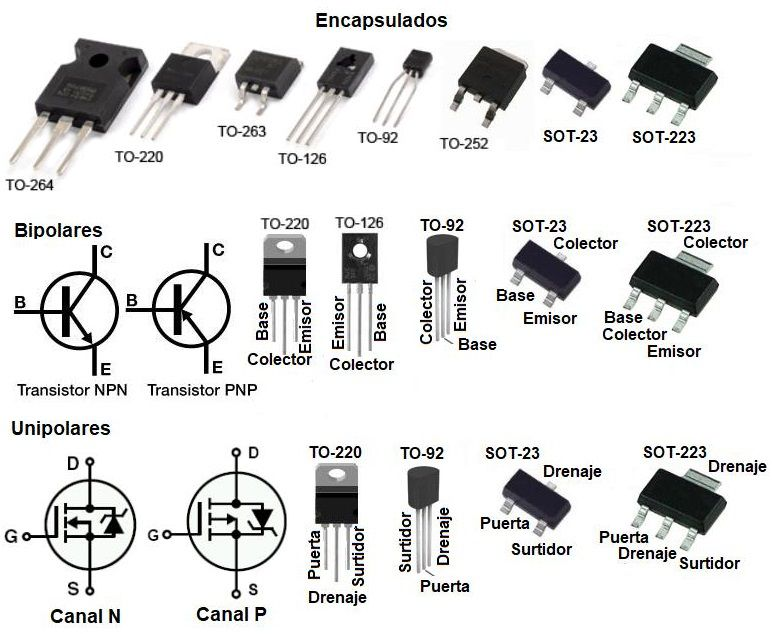
\includegraphics[width=0.35\textwidth]{Imagenes/transistores.jpg}
    \caption{Tipos de transistores}
    \label{fig:transistores}
\end{wrapfigure}

El transistor o BJT es un componente eléctrico semi-conductor que puede ser utilizado para el control adecuado del flujo de corriente eléctrica.


En este caso, una pequeña cantidad de corriente en el conductor base, puede controlar una mayor cantidad de corriente entre el colector y el emisor.

Es por ello que los transistores son muy utilizados en la actualidad para amplificar una señal algo débil (un oscilador o un interruptor, por ejemplo).

En resumen, un transistor puede modificar una señal eléctrica de salida en respuesta a una de entrada, funcionando de esta forma como conmutador, amplificador, rectificador u oscilador.

Entre las características más destacadas de un transistor tenemos:
\begin{itemize}
    \item Es un dispositivo electrónico semiconductor.
    \item Permite el paso de una señal (salida) en respuesta a otra (entrada).
    \item Suelen estar fabricados de cristal de silicio.
    \item Los transistores son sellados herméticamente.
    \item Presentan una carcasa de plástico o una cubierta metálica con tres terminales.
    \item Se puede configurar como amplificador, conmutador, oscilador, o rectificador.
\end{itemize}

\subsubsection{¿Para qué sirven?}

Como ya hemos indicado anteriormente, los transistores son un tipo de dispositivo electrónico que pueden controlar o modificar el flujo de electricidad, siendo ideales para alimentar otros dispositivos pequeños y potentes.

Estos pequeños componentes se elaboran mayormente de silicio y se utilizan en diversos tipos de aparatos electrónicos: teléfonos móviles, tabletas industriales, computadores y robots en las industrias.

Por lo tanto, los transistores tienen diversas aplicaciones en la electrónica y en muchas otras industrias, revolucionado la forma de interactuar entre la tecnología y las actividades cotidianas.
Sin duda, los transistores son un componente muy importante para la industria moderna, ya que permiten circuitos más pequeños y eficientes, y también se pueden usar para diseñar dispositivos digitales de última tecnología.
Adicionalmente, no olvidemos que los transistores pueden ser de tipo “activados o no activados”, y básicamente se diferencian en la forma en que funciona cada uno de ellos.

\subsubsection{¿Cómo funciona un transistor?}
El objetivo principal de un transistor es permitir la transferencia adecuada de energía eléctrica entre las diferentes partes de un circuito eléctrico.

Por lo tanto, los transistores controlan o cambian el flujo de electricidad entre dos puntos, y vienen en muchas formas y tamaños.

Los transistores se utilizan en todo tipo de aparatos electrónicos: desde teléfonos móviles y tabletas, hasta computadores y robots en las industrias.

En términos generales, estos trabajan sobre un flujo de corriente, funcionando como amplificadores al recibir una señal débil y generando una señal más fuerte, o como interruptores al recibir una señal y cortar su paso.

Normalmente, esto ocurre dependiendo de las posiciones que ocupe un transistor en un determinado instante:
\begin{itemize}
    \item \textbf{Posición activa}: aquí se permite el paso de un nivel de corriente variable
    \item \textbf{En corte}: en esta posición no se deja pasar la corriente eléctrica
    \item \textbf{En saturación}: aquí se deja pasar toda la corriente eléctrica (corriente máxima)
\end{itemize}



En cuanto a las partes de un transistor, este se compone de 3 elementos clave: hablamos de la base, colector y emisor.

En ese caso, la base intercede entre el emisor por donde entra la corriente y el colector por donde sale el caudal de corriente.  Es por ello que, si la base de un transistor no recibe corriente eléctrica, este se ubicará en posición de corte. En cambio, si el transistor recibe un flujo de corriente intermedia, la base puede abrir el flujo en una determinada cantidad.

Y, por último, si la base recibe un gran flujo de corriente eléctrica, entonces se abrirá al máximo para pasar el total de la corriente modulada.

Ahora, teniendo un conocimiento previo de lo que es un transistor, se puede saber un poco más sobre como de ese pequeño dispositivo, se puede realizar un análisis detallado de sus configuraciones mas importantes y de ellos crear las etapas que se estudiarán mas adelante.

\subsection{Corrientes del transistor BJT}

Se debe tener en cuenta lo siguiente con las corrientes de los transistores:


\subsubsection{Corriente de colector}
\begin{equation}
    I_C=\beta I_B
    \label{eqn:ic}
\end{equation}
\subsubsection{Corriente de base}
\begin{equation}
    I_B=\dfrac{I_C}{\beta }
    \label{eqn:ib}
\end{equation}
\subsubsection{Corriente de emisor}
\begin{align}
    I_E & =I_B+I_C \label{eqn:ie}                                                                       \\[0.2cm]
    I_E & =\dfrac{I_c}{\beta}+I_C=(\dfrac{1}{\beta}+1)I_C =\dfrac{1+\beta}{\beta}I_C  \label{eqn:ie_ic} \\[0.2cm]
    I_E & = I_B+\beta I_B = I_B(1+\beta) \label{eqn:ie_ib}
\end{align}
\subsection{Configuraciones básicas del BJT}

Los transistores son uno de los componentes más utilizados dentro de la electrónica ya que tienen diferentes configuraciones y polarizaciones, y dependiendo de las variaciones estos funcionan de forma diferente. Cuando se quiere utilizar un transistor como interruptor digital (regiones de corte y saturación) la tarea es fácil ya que el circuito eléctrico es bastante sencillo. En caso de que se utilicé un transistor NPN el emisor se coloca a tierra, el colector a voltaje y la base actúa como interruptor, o si bien se utiliza un transistor PNP se invierten las terminales, el colector a tierra y al emisor se le pone voltaje.

\begin{figure}[H]
    \centering
    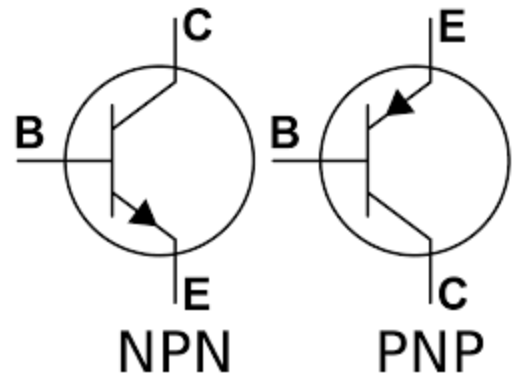
\includegraphics[width=5cm]{Imagenes/simbolo_bjt.png}
    \caption{Símbolo esquemático para cada unos de los transistores BJT}
    \label{fig:simbologia}
\end{figure}

\subsubsection{Emisor Común (EC)}

Esta configuración se utiliza para amplificadores de corriente y voltaje a bajas frecuencias, debido a que tiene una alta ganancia en las dos variables. Una de sus características no tan favorables es que el voltaje de la señal queda invertido en su salida (la corriente no se invierte), es decir las señales quedan como si fueran un espejo. Una forma sencilla de identificar esta configuración es por que la señal de entrada esta en la base y la de salida en el colector. Esta configuración se puede utilizar con todos los tipos de polarizaciones.

\subsubsection{Colector Común (CC)}

Se utiliza para señales con baja potencia y las transforma en el mismo tipo de señal pero con una mayor potencia. Esto se logra por que tiene una alta ganancia de corriente y el voltaje lo transfiere igual ya que no tiene ganancia de voltaje. Otra característica es que en la salida se invierte la corriente. El colector común se utiliza principalmente cuando se requiere poner varios amplificadores conectados en serie debido a que en su entrada tiene mucha impedancia y en su salida disminuye.


\subsubsection{Base Común (BC)} Existen dos formas sencillas de identificar si un transistor esta configurado en base común y estas son; por que el símbolo del transistor se utiliza acostado o porque la entrada es a través del emisor y la salida se encuentra en el colector. A pesar de que esta configuración no tiene una ganancia de corriente se utiliza por que el ancho de banda es más grande que las demás configuraciones y permite trabajar con señales VHF (very high frequency) y UHF (ultra high frequency).


\begin{figure}[H]
    \centering
    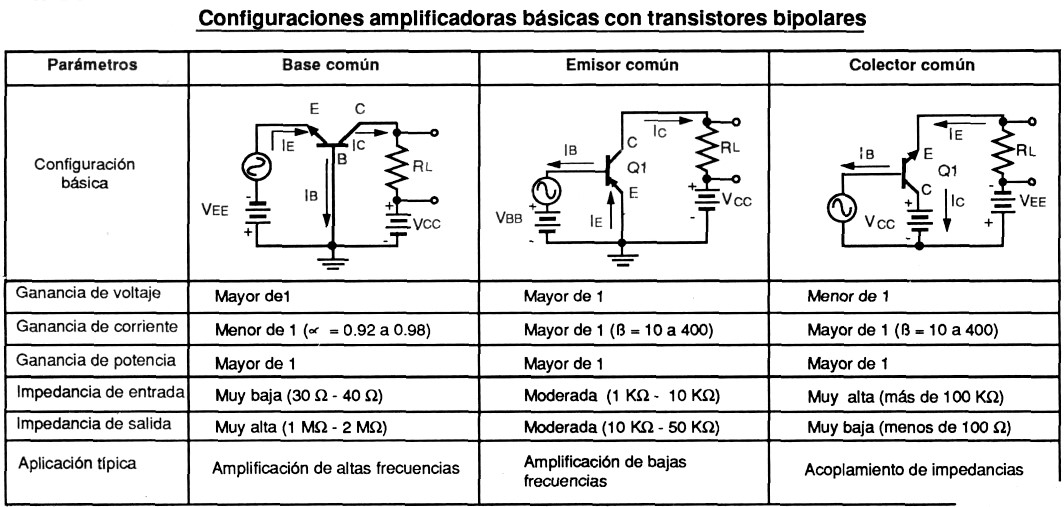
\includegraphics[width=\textwidth]{Imagenes/Configuraciones BJT basicas.jpg}
    \caption{Resumen de configuraciones de los transistores}
    \label{fig:configuraciones}
\end{figure}

Para el cálculo del modelo pi las ecuaciones son distintas
dependiendo su configuración (EC, CC o BC)

\subsection{Polarizaciones de un transistor BJT}

En simples palabras las polarizaciones son circuitos que se utilizan para hacer funcionar a los transistores como amplificadores, en estos circuitos basan su funcionamiento en las configuraciones anteriores, ya que podemos utilizar una de emisor común y utilizar cualquiera de las polarizaciones disponibles todo depende de la aplicación que se le dé al transistor.

\subsubsection{Polarización fija o de base}
Esta polarización solo se puede utilizar con la configuración de emisor común y consiste en colocar una resistencia en la base y una en el colector, mientras que el emisor se conecta a tierra, Al ser una configuración demasiado sencilla tenemos una gran desventaja y es que la señal esta muy expuesta a variaciones dependiendo de los cambios de temperatura que tenga el transistor. Regularmente se utiliza para señales de poca importancia que no importa que se distorsionen.

\subsubsection{Polarización por retroalimentación del emisor o estabilizado en el emisor}
En este tipo prácticamente se le agrega una resistencia en el emisor que hace sea un poco más estable, pero no lo suficiente como para utilizarlo en señales de mucha importancia.

\subsubsection{Polarización por retroalimentación de colector}
Prácticamente se utiliza para regular los cambios de corriente o de voltaje en la fuente de alimentación, ya que si por alguna razón existe una variación, la resistencia que retroalimenta la base actúa para evitar un cambio brusco en la salida del transistor.

\subsubsection{Polarización universal o divisor de voltaje}
Es la más utilizada ya que es la más estable, debido a sus retroalimentaciones. Y si por cualquier razón el transistor se calienta o existen una variación de la corriente la resistencias de retroalimentación actúan para regular la corriente que llega a la base y así poder estabilizar todo el sistema.

\begin{figure}[H]
    \centering
    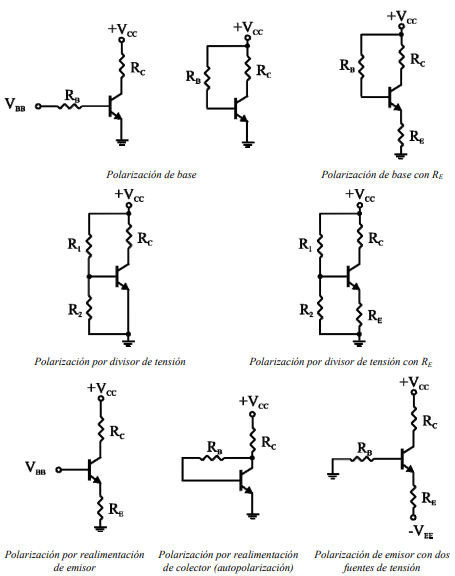
\includegraphics[width=\textwidth]{Imagenes/polarizacion.png}
    \caption{Diferentes circuitos empleados en la polarización de un transistor}
    \label{fig:polarizacion}
\end{figure}

\begin{figure}[H]
    \centering
    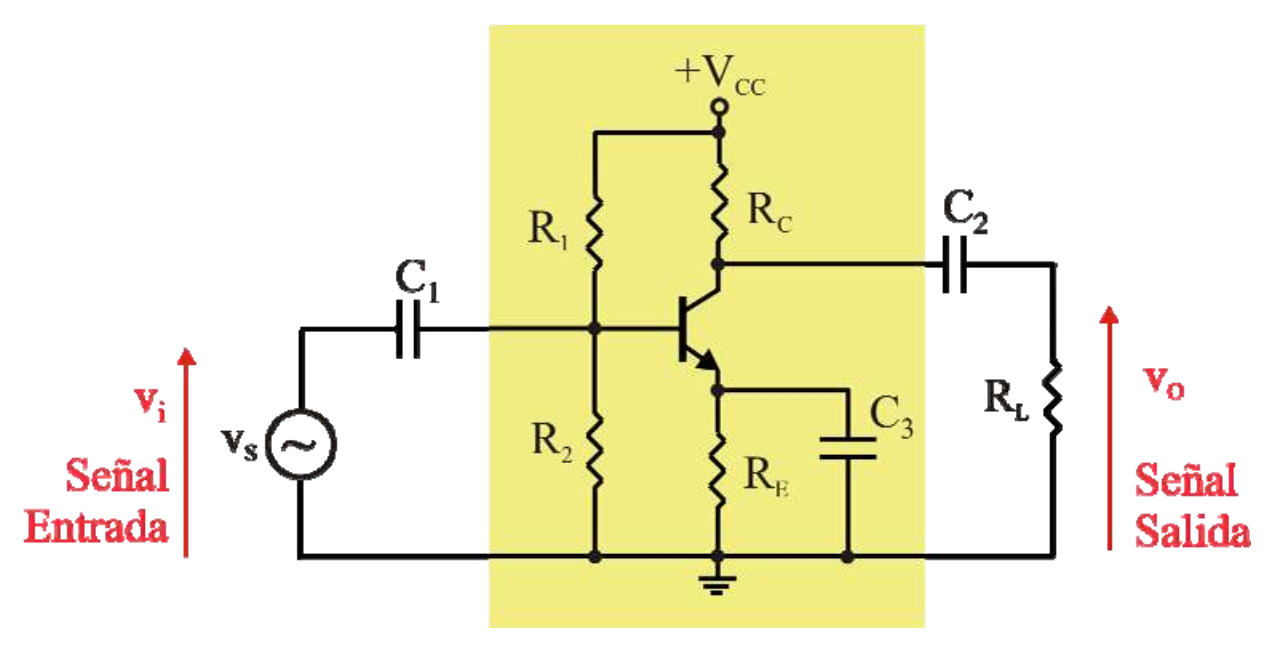
\includegraphics[width=\textwidth]{Imagenes/bjt_ec.png}
    \caption{Circuito amplificador de tensión con BJT en EC}
    \label{fig:ec}
\end{figure}

\subsection{Condensadores de acople y desacople}
En el circuito de la figura \ref{fig:ec} se muestra un circuito típico de un amplificador de tensión con un transistor BJT en emisor común polarizado en la zona activa.
Con él se trata de amplificar una tensión cualquiera vi y aplicarla, una vez amplificada, a una carga que simbolizamos por la resistencia RL. La zona sombreada
resalta el amplificador, que en este caso, lo constituye un transistor BJT en la configuración emisor común. El cual, convenientemente polarizado en la zona activa, es
capaz de comportarse como un amplificador de tensión como ya se mencionó anteriormente.

Los condensadores $C_1$ y $C_2$ que aparecen se denominan condensadores de acoplo y sirven para bloquear la componente continua. En concreto $C_1$ sirve para acoplar la tensión que queremos amplificar al amplificador propiamente dicho, eliminando la posible componente continua que esta tensión pudiera tener. Si no bloqueásemos esta continua se sumaría a las corrientes de polarización del transistor modificando el punto
de funcionamiento del mismo. Por otra parte, el condensador $C_2$ nos permite acoplar la señal amplificada a la carga, eliminando la componente continua (la correspondiente al punto de polarización del transistor) de forma que a la carga llegue únicamente la componente alterna.

El condensador $C_3$ es un condensador de desacoplo, su misión es la de proporcionar un camino a tierra a la componente alterna. En el capítulo anterior se
analizó el efecto de la resistencia $R_E$ desde el punto de vista de su efecto en la estabilización del punto de polarización. Sin embargo, en este capítulo veremos como
desde el punto de vista de la amplificación, esta resistencia hace disminuir la ganancia del amplificador. Al añadir el condensador de desacoplo conseguimos que la continua pase por $R_E$ mientras que la alterna pasaría por el condensador $C_3$ consiguiendo que no
afecte a la amplificación.

\subsection{Principio de superposición}
En este informe vamos a abordar el análisis de este tipo de circuitos amplificadores. Para ello aplicaremos el principio de superposición. En cada punto o rama calcularemos las tensiones y corrientes de continua y de alterna por separado, de forma que al final las tensiones y corrientes finales serán la suma de las calculadas en
cada parte.

Para ello vamos a suponer que el valor de la capacidad de los condensadores, así como la frecuencia de las señales que tenemos es tal que la impedancia que presentan
los condensadores es lo suficientemente pequeña para considerarla nula. Mientras que en continua, estos condensadores presentarán una impedancia infinita. Es decir, consideraremos que en continua los condensadores se comportan como circuitos abiertos (impedancia $\infty$) mientras que en alterna equivaldrán a cortocircuitos (impedancia $0$)

\begin{equation}
    |x_c|=\dfrac{1}{\omega \cdot C}=\dfrac{1}{2\pi f \cdot C}
    \label{eqn:capacitores}
\end{equation}

\begin{figure}[H]
    \centering
    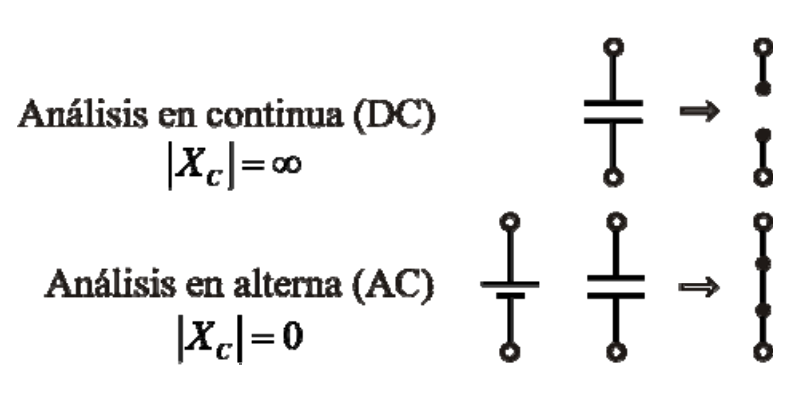
\includegraphics[width=8cm]{Imagenes/analisis_condensadores.png}
    \caption{Consideraciones para aplicar el principio de superposición.}
    \label{fig:consideraciones}
\end{figure}

Aplicando estas consideraciones obtendremos los circuitos equivalentes en DC y en AC que tendremos que resolver separadamente.

Si en el circuito amplificador de la figura \ref{fig:ec} aplicamos la condición de que los condensadores se comportan como circuitos abiertos, obtenemos el circuito equivalente en continua (figura \ref{fig:universal}). Podemos ver como este circuito es, precisamente, el circuito de polarización del transistor cuyo estudio ya se abordó en el punto anterior y de cuya
resolución obtendríamos las tensiones y corrientes de continua presentes en el circuito.

\begin{figure}[H]
    \centering
    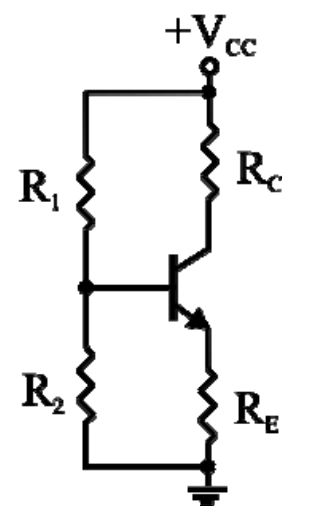
\includegraphics[width=3cm]{Imagenes/universal.png}
    \caption{Circuito equivalente en DC de la figura \ref{fig:ec}}
    \label{fig:universal}
\end{figure}

\subsection{Punto de operación Q}

El punto de operación, es un punto fijo sobre las curvas características, se le conoce también como punto quiesciente (abreviado punto Q). Por definición, quiescente significa quieto, inmóvil, inactivo.

En general, lo importante es calcular los valores de voltajes y corrientes del transistor para una polarización dada. Por tal motivo, se agregara la letra Q a cada
una de los términos que se desean obtener y que son: la corriente de base $I_{BQ}$; la corriente de colector $I_{CQ}$; la corriente de emisor $I_{EQ}$; el voltaje base-emisor $V_{BEQ}$ y el voltaje colector-emisor $V_{CEQ}$. En la mayoría de los casos, la corriente de base $I_{BQ}$ es la primera cantidad que se determina junto con el voltaje base emisor $V_{BEQ}$, una vez que $I_{BQ}$ se conoce, las relaciones de las ecuaciones de malla pueden aplicarse para encontrar las restantes variables como la corriente de colector $I_{CQ}$, etc. Las similitudes en los análisis serán inmediatamente obvias y
las ecuaciones son tan similares para diversas configuraciones que una ecuación
de malla puede derivarse de otra quitando o agregando términos.

\subsection{\texorpdfstring{Modelo $\pi$}{Modelo pi}} %Esta sintaxis es para que no tengo errores al ser referenciado por el entorno hyperref.


\subsubsection{Modelo Pi-híbrido básico del transistor BJT}
Antes de pasar a estudiar el modelo Pi híbrido del transistor voy a compartir un diagrama con la nomenclatura asociada al transistor BJT, con las terminales y las corrientes y voltajes de interés en este dispositivo.

\begin{figure}[H]
    \centering
    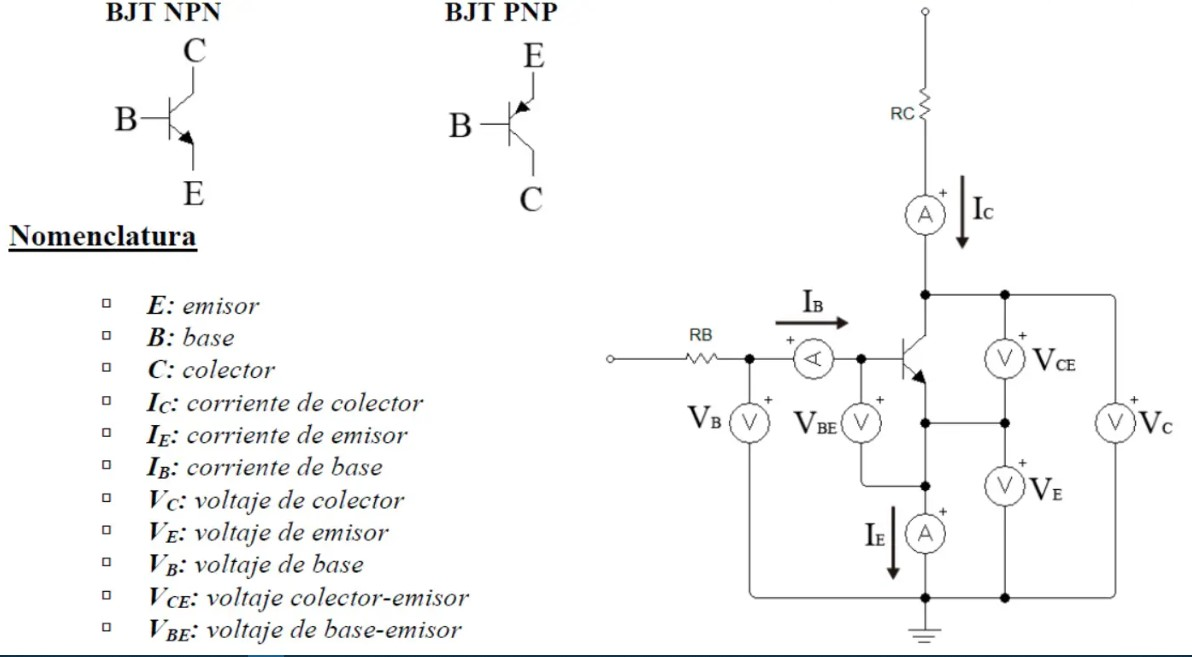
\includegraphics[width=\textwidth]{Imagenes/bjt.jpg}
    \caption{Nomenclatura del BJT}
    \label{fig:bjt}
\end{figure}

Es importante conocer estos términos y como calcularlos, pues de ello dependerá el Modelo Pi. El modelo Pi-híbrido es un modelo de circuito eléctrico que te permite remplazar un transistor en un circuito electrónico por un circuito basado en una fuente dependiente, que facilita el análisis del comportamiento del transistor en condiciones cuando se aplica una señal de frecuencia variable en la entrada del transistor. Básicamente es una convención que permite analizar circuitos con transistores en condiciones de corriente alterna.

Para usar el modelo Pi será necesario remplazar el transistor por un modelo equivalente, el cual se muestra a continuación:

\begin{figure}[H]
    \centering
    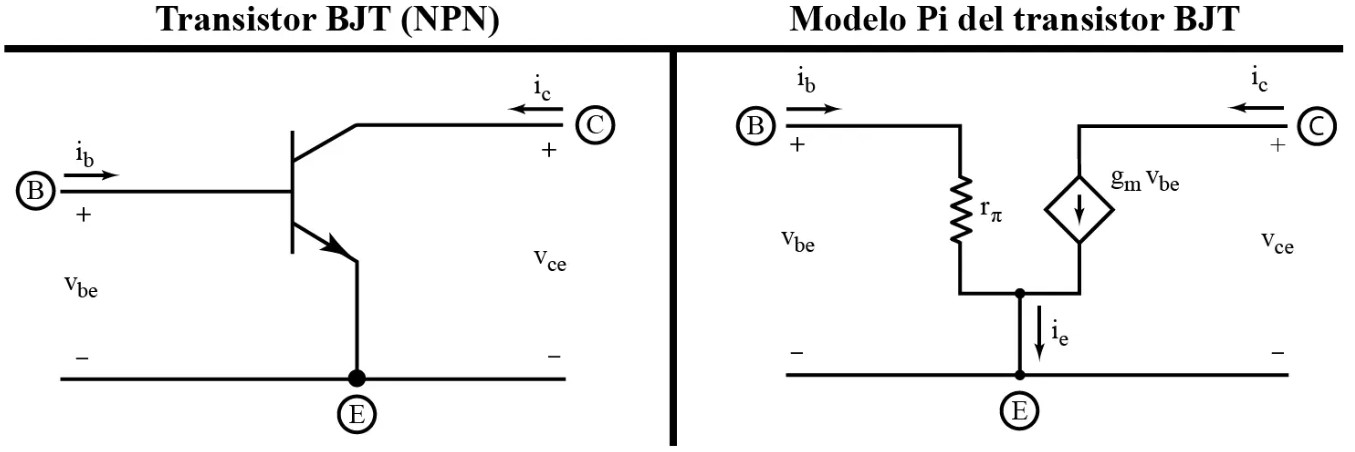
\includegraphics[width=10cm]{Imagenes/modelopi.jpg}
    \caption{Modelo $\pi$}
    \label{fig:modelo_pi}
\end{figure}

Para utilizar el modelo Pi, hace falta calcular dos parámetros: la resistencia $\pi$ y la transconductancia \textbf{$g_m$}. Estos parámetros se calculan utilizando las siguientes ecuaciones:

\begin{gather}
    \mathbf{r_{\pi}} = \dfrac{V_{be}}{i_b} = \dfrac{V_T}{I_{BQ}} = \beta \dfrac{V_T}{I_{CQ}} \label{eqn:rpi}
\end{gather}

\begin{gather}
    \mathbf{g_m}= \dfrac{I_{CQ}}{V_T} \label{eqn:gm}
\end{gather}

En estas ecuaciones la $\beta$ es la ganancia del transistor, la cual es un dato del propio transistor. Este dato casi siempre lo proporciona el enunciado del problema que estemos trabajando. $v_T$ es el voltaje térmico, el cual es aproximadamente 0.026 voltios a la temperatura ambiente (27 ºC). Los sub índices que contienen Q hacen referencia a condiciones de carga.

\subsubsection{Voltaje térmico}

El voltaje térmico ($V_T$) de un transistor bipolar de juntura (BJT) es un parámetro importante que se refiere a la tensión necesaria para mantener una corriente específica en el transistor. Este parámetro es fundamental para entender el comportamiento del transistor en diferentes condiciones de temperatura y corriente.

Se define como la tensión necesaria para mantener una corriente específica en el transistor, usualmente medida entre el colector y la base. Este parámetro es importante porque la temperatura del transistor puede afectar su comportamiento, y el voltaje térmico es una medida de cómo se ajusta la tensión para compensar estos cambios.

\begin{itemize}
    \item Efecto de la temperatura

          Cuando la temperatura del transistor aumenta, la corriente de colector también aumenta debido a que la cantidad de portadores minoritarios en el material semiconductor aumenta. Esto se traduce en un aumento en la corriente de colector. El voltaje térmico se ajusta para compensar este aumento, manteniendo constante la corriente de colector.
    \item Importancia en el diseño

          El voltaje térmico es crucial en el diseño de circuitos que utilizan transistores BJT, ya que permite ajustar la tensión para mantener constante la corriente en diferentes condiciones de temperatura. Esto es especialmente importante en aplicaciones que requieren estabilidad y precisión, como en sistemas de control y amplificación.
\end{itemize}

Siguiendo la siguiente ecuación:

\begin{gather}
    V_T=\dfrac{K \, T}{q}
\end{gather}

Donde, \\
$K$: Constante de Boltzmann $= 1.3806 \, x 10^{-23}$. \\
$q$: Carga del electron $= 1.609 \,x 10^{-19}$. \\
$T$: Temperatura ambiente (en Kelvin) $=25^{\circ} C=298.15 Kelvin$

Teniendo todas las condiciones adecuadas, el valor del voltaje térmico es de $V_T=25.865 m\volt$

\subsubsection{Forma expandida del modelo Pi-híbrido}

El modelo Pi-híbrido expandido toma en cuenta algunos efectos que se producen cuando el transistor opera en condiciones de frecuencia variable y altas frecuencias. A continuación se presenta el modelo Pi-híbrido expandido:

\begin{figure}[H]
    \centering
    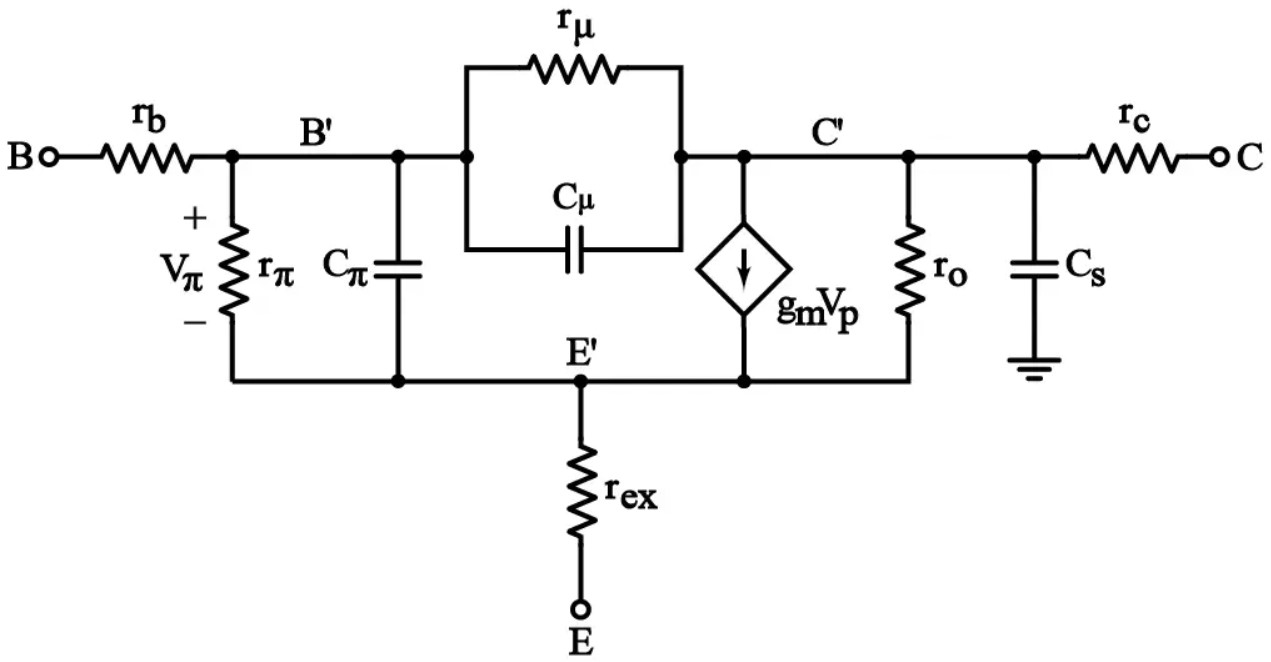
\includegraphics[width=10cm]{Imagenes/modelo pi wh.jpg}
    \caption{Modelo $\pi$ en altas frecuencias}
    \label{fig:modelo_pi_2}
\end{figure}

A continuación procedemos a describir cada uno de los elementos de este modelo:

\begin{itemize}
    \item \textbf{$r_b$, $r_c$, $r_{ex}$:} son resistencias parásitas que se forman en la base, colector y emisor del transistor. Estas resistencias quedan conectadas en serie a las resistencias de base (\textbf{$r_b$}), colector (\textbf{$r_c$}) y emisor (\textbf{$r_{ex}$}). Típicamente poseen valores bajos, entre 1$\Omega$ y 2$\Omega$, por lo cual pueden ser despreciadas.
    \item\textbf{$C_s$:} es la capacitancia del sustrato con el que se construye el transistor. Normalmente posee un valor despreciable. En inglés se conoce como \textbf{junction capacitance of the reverse biased collector–substrate junction}.
    \item\textbf{$C_{\pi}$ y $C_{\mu}$:} son capacitancias asociadas a la juntura del transistor. En inglés se conocen como \textbf{forward-biased junction capacitance o input capacitance} y \textbf{reverse-biased junction capacitance o output capacitance}, respectivamente. Normalmente $C_{\mu}$ es mucho más pequeña que $C_{\pi}$. Sin embargo, por un efecto llamado \textbf{Efecto Miller}, esta capacitancia no puede ser despreciada.

    \item \textbf{$r_\pi$ y $r_{\mu}$:} son resistencias que aparecen en el modelo de corriente alterna. \textbf{$r_{\pi}$} ya la conocemos y sabemos calcularla; \textbf{$r_{\mu}$} es una resistencia con un valor muy alto, típicamente en el orden de los megaohms, por lo cual puede ser despreciada.
\end{itemize}

Algunos de los valores mostrados en el modelo expandido son despreciables por tratarse de resistencias (similar a un circuito abierto) o muy pequeñas (similar a un corto circuito).

\subsubsection{Modelo Pi con efecto Early}

El voltaje Early (denotado por $V_A$) es otro dato del transistor. Es un voltaje que se ubica entre $50$ y $300 V$ y está asociado a la pendiente de las curvas de de polarización del transistor. Este voltaje produce una resistencia denotada por ro que se ubica en la salida del modelo equivalente del transistor, es decir, entre colector y emisor.

\begin{figure}[H]
    \centering
    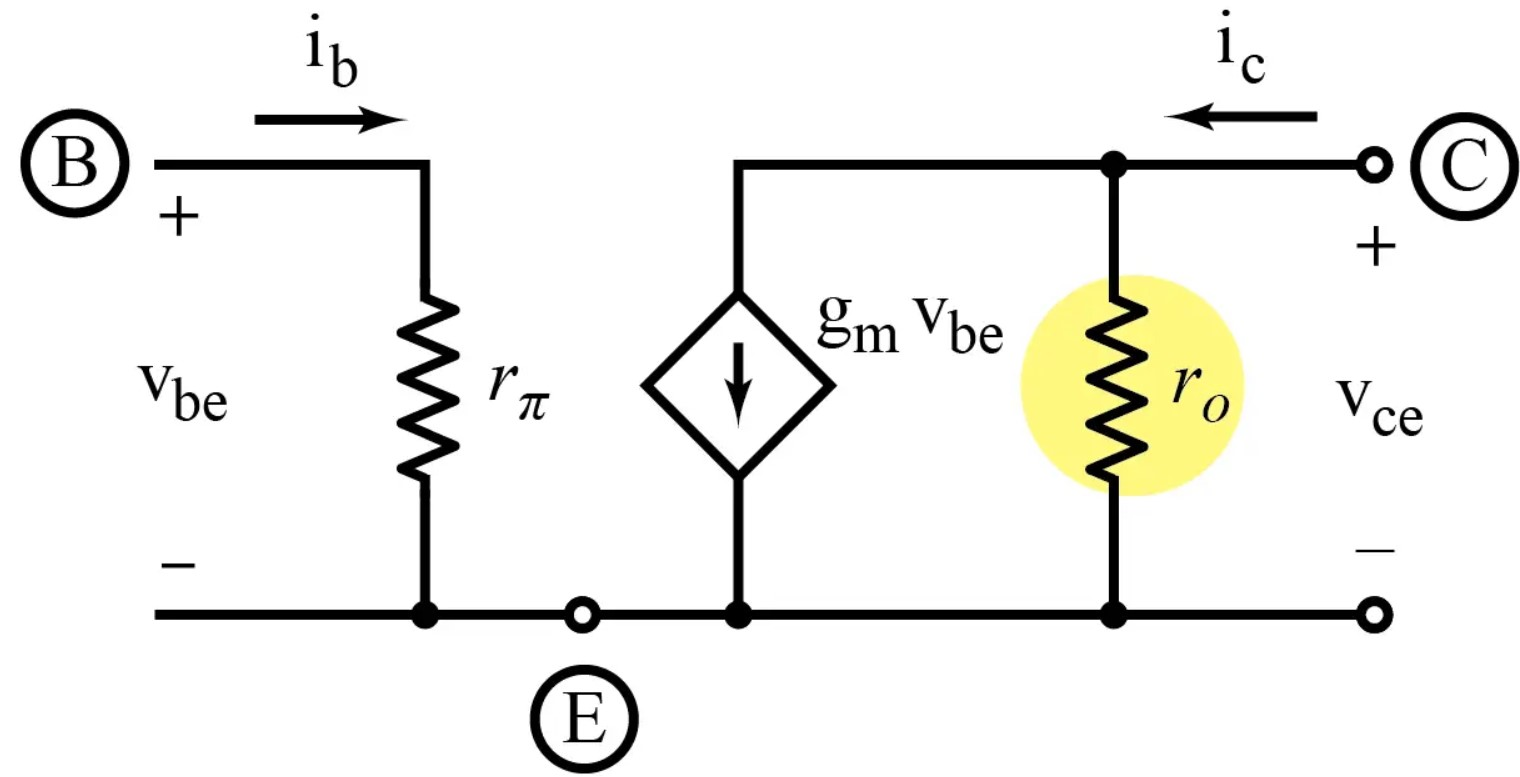
\includegraphics[width=8cm]{Imagenes/modelo_pi3.jpg}
    \caption{Modelo $\pi$ con efecto Early}
    \label{fig:modelo_pi3}
\end{figure}

Para calcular la resistencia $r_o$ se utiliza la siguiente ecuación:

\begin{gather}
    \mathbf{r_o} = \dfrac{V_{A}}{I_{CQ}} \label{eqn:ro}
\end{gather}

Esta resistencia normalmente es de un valor alto, razón por la cual es posible despreciarla. Todo dependerá si se cuenta con un valor de $V_A$, el cual es un dato proporcionado en el enunciado del problema. En otras palabras, es un dato de la hoja de datos del propio transistor.

\subsection{Teorema Miller}

El Teorema de Miller permite redefinir el modelo de corriente alterna del BJT para considerar el efecto de la capacitancia $C_{\mu}$, la cual ya mencionamos en las secciones anteriores de este documento. Sin entrar mucho en detalles, el Teorema de Miller permite hacer lo siguiente:


\begin{figure}[H]
    \centering
    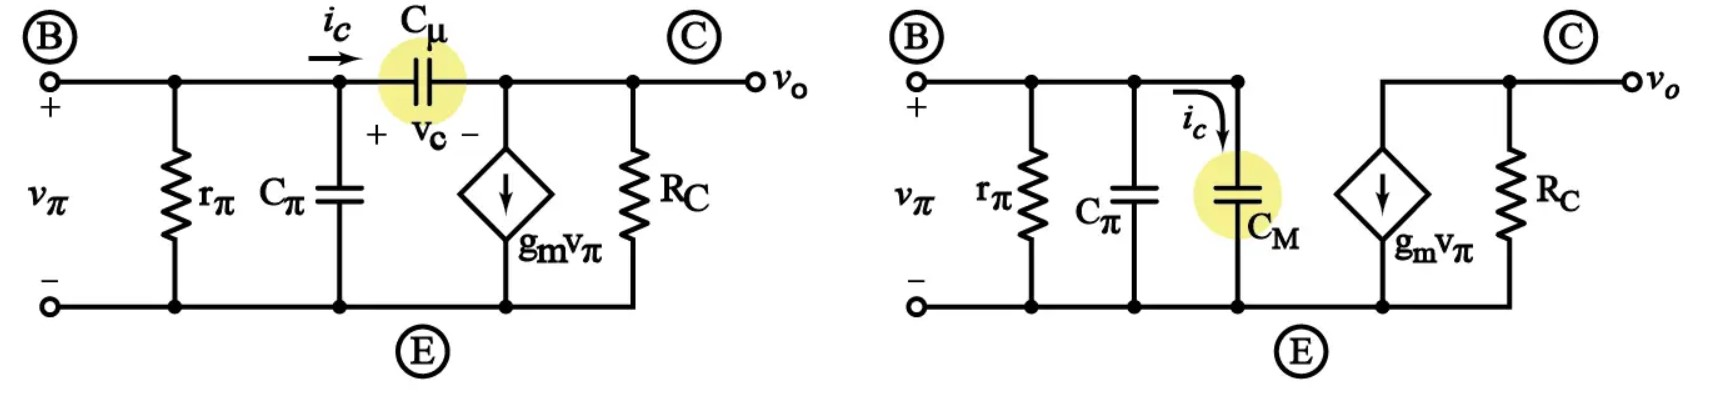
\includegraphics[width=\textwidth]{Imagenes/teorema_miller.jpg}
    \caption{Modelo $\pi$ en altas frecuencias equivalente por el Teorema Miller}
    \label{fig:miller}
\end{figure}

Para hacer la conversión de $C_{\mu}$ a $C_M$ se utiliza la siguiente ecuación:

\begin{equation}
    \mathbf{C_M} =  C_{\pi} + C_{\mu}(1+g_mZ_{out}) = C_{\mu}(1+|A_v|) = \mathbf{C_{eq}} \label{eqn:C_eq}
\end{equation}

En esta ecuación $A_v$ es la ganancia de voltaje del amplificador. Esta ganancia se obtiene al dividir el voltaje de salida entre el voltaje de entrada.

\subsubsection{Resistencia de difusión o intrínseca del emisor ($r_x$)}

$r_x$ en el contexto de transistores bipolares puede referirse a la resistencia de difusión ($r_e$ o resistencia intrínseca del emisor) en el modelo híbrido, no es una nomenclatura estándar comúnmente utilizada en los datasheets de los transistores.

Para calcular la resistencia de difusión se usa la siguiente formula:

\begin{gather}
    r_x=\dfrac{V_T}{I_{E}} \label{eqn:rx}
\end{gather}



\subsection{Ganancia de un amplificador}

Debido a que los amplificadores tienen la capacidad de aumentar la magnitud de una señal de entrada, es útil poder calificar la capacidad de amplificación de un amplificador en términos de una relación salida/entrada. El término técnico para la relación de magnitud salida/entrada de un amplificador es ganancia. Como una relación de unidades iguales (salida de energía/entrada de energía, salida de voltaje/ entrada de voltaje o salida de corriente/entrada de corriente), la ganancia es naturalmente una medición sin unidades.

Matemáticamente, la ganancia está simbolizada por la letra mayúscula “A”.

Las ganancias del amplificador eléctrico se pueden expresar en términos de voltaje, corriente y/o potencia tanto en CA como en CC.

Un resumen de las definiciones de ganancia es el siguiente:

El símbolo “delta” en forma de triángulo ($\triangle$) representa el cambio en las matemáticas, por lo que “$\triangle$V output/$\triangle$V input” significa “cambio en el voltaje de salida dividido por el cambio en el voltaje de entrada”, o más simplemente, “voltaje de salida AC dividido por voltaje de entrada AC”:

\begin{figure}[H]
    \centering
    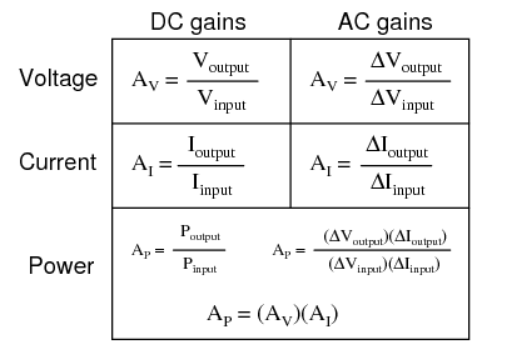
\includegraphics[width=8cm]{Imagenes/gain_amp.png}
    \caption{Distintas Ganancias de un amplificador}
    \label{fig:gain_amp}
\end{figure}

La siguiente ecuación es la mas usada en este capitulo,

\begin{equation}
    A_v=\dfrac{v_o}{V_{in}}
    \label{eqn:av}
\end{equation}





\subsection{Etapas de un amplificador base}
\subsubsection{Amplificador diferencial}
La mayoría de los amplificadores operativos modernos utilizan un extremo frontal de amplificador diferencial. En otras palabras, la primera etapa del amplificador operacional es un amplificador diferencial.

El amplificador diferencial es un circuito que forma parte fundamental de muchos amplificadores y comparadores.

Es un dispositivo que aumenta la diferencia entre dos voltajes de entrada, pero que destruye cualquier voltaje común a dichas entradas. Se trata de un circuito analógico con dos entradas denominadas entrada inversora y entrada no inversora y una sola salida proporcional a la diferencia entre los dos voltajes.

Algunos fabricantes llaman a este instrumento como par diferencial.

En el amplificador diferencial ideal la salida depende de la diferencia de las señales de entrada:

\begin{equation}
    V_o=V_d A_d
\end{equation}

Siendo $V_d$ la señal diferencial y  $A_d$ la ganancia diferencial.

En el amplificador diferencial real la salida depende además de la señal común de ambas entradas:

\begin{equation}
    V_o=V_d A_d+ V_c A_c
\end{equation}

$V_c$ es la señal en modo común
\begin{equation}
    V_c = \dfrac{V_1+V_2}{2}
\end{equation}

$A_c$ es la ganancia en modo común.
A continuación en la figura \ref{fig:diferencial} se muestra la configuración básica de este amplificador.

\begin{figure}[H]
    \centering
    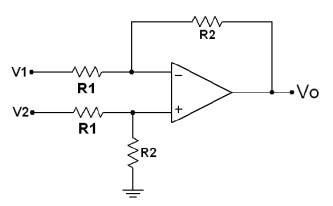
\includegraphics[width=8cm]{Imagenes/diferencial.png}
    \caption{Configuración básica Amplificador Diferencial}
    \label{fig:diferencial}
\end{figure}

Es un montaje simétrico, son dos etapas en emisor común con acoplamiento directo en el emisor.
Las señales de entrada $V_1$ y $V_2$ se aplican en las bases y las señales de salida $V_{o1}$ y $V_{o2}$ se toman en los colectores.
Tenemos:

\begin{align}
    \text{Salida Diferencia:} &  & V_o=V_{o2}-V_{o1} \\
    \text{Salida Asimétrica:} &  & V_o=V_{o2}
\end{align}

\begin{itemize}
    \item \textbf{Ganancia modo diferencial}

          \begin{equation}
              A_d=-\dfrac{V_o}{Z_d}
              \label{eqn:ad}
          \end{equation}


    \item \textbf{Ganancia modo común}

          \begin{equation}
              A_c=-\dfrac{V_o}{Z_c}
              \label{eqn:ac}
          \end{equation}


    \item \textbf{Relación de Rechazo en Modo Común (CMRR)}
          \begin{equation}
              CMRR=\rho=20\cdot log \left| \dfrac{A_d}{A_c}\right|
              \label{eqn:cmrr}
          \end{equation}
\end{itemize}


En la salida diferencial el comportamiento es ideal.
En la salida asimétrica tendremos buen comportamiento si la resistencia $R_E$ es alta ya que con eso conseguimos que $A_c$ sea baja. Cuanto más baja sea $A_c$
más se asemejará al comportamiento ideal.

Para el cálculo de la Relación de rechazo del modo común:

$V_c$ es la señal en modo común

\subsubsection{Amplificador de la etapa elevadora o driver o impulsora}

La etapa de elevación está diseñada para manejar grandes corrientes y voltajes, lo que permite al amplificador operacional manejar cargas pesadas y proporcionar una salida estable y confiable. Esta etapa se compone de transistores bipolares que trabajan en configuración push-pull, lo que significa que un transistor se encarga de manejar la corriente positiva mientras que el otro maneja la corriente negativa. Esto permite una mayor eficiencia y estabilidad en la salida.

La etapa de elevación es fundamental para el funcionamiento del amplificador operacional ya que:

\begin{itemize}
    \item \textbf{Manejo de cargas pesadas}

          La etapa de elevación permite al amplificador operacional manejar cargas pesadas sin perder su capacidad de amplificación.

    \item \textbf{Estabilidad de la salida}

          La etapa de elevación ayuda a mantener la estabilidad de la señal de salida, asegurando que no haya fluctuaciones indeseadas.

    \item \textbf{Amplificación de señales}

          La etapa de elevación es responsable de amplificar la señal de entrada para proporcionar una salida lo suficientemente fuerte para manejar las cargas externas.

\end{itemize}

\subsubsection{Amplificador de potencia}
Un amplificador de potencia es un amplificador electrónico diseñado para aumentar la magnitud de potencia de una señal de entrada.

A diferencia de los amplificadores de voltaje y corriente, un amplificador de potencia está diseñado para impulsar cargas, y se establece como bloque final en un circuito amplificador.

Entre las aplicaciones más frecuentes de un amplificador de potencia destacan:

\begin{itemize}
    \item Medición de valores de impedancia muy bajos.
    \item Medición de impedancia dependiente del voltaje.
    \item Dotar de más potencia en los circuitos durante la medición de impedancia de entrada o de salida.
    \item Generar más energía en entornos ruidosos, como mediciones en convertidores de CC/CC de alta potencia o convertidores de CA/CC.
\end{itemize}

\paragraph{Clases de amplificadores de potencia}

Los amplificadores de potencia más comunes son los que se utilizan en los circuitos de amplificadores de audio y vienen en clases A, B, AB o C.

\subparagraph{Amplificador de potencia clase A:}

En el amplificador de potencia de la clase A, toda la forma de onda de entrada se usa en el proceso de amplificación. Por lo que son los amplificadores de potencia de uso más comunes.

En los amplificadores de potencia de clase A, un único transistor se usa para amplificar las mitades positiva y negativa de la forma de onda. Por otro lado, su ángulo de conducción es de 360º, por lo que los niveles de distorsión de señal son muy inferiores y permiten un mejor rendimiento de alta frecuencia. Sin embargo, una de las principales desventajas de los amplificadores de potencia y especialmente del amplificador de Clase A es que su eficiencia de conversión general es muy baja, ya que las grandes corrientes significan que se pierde una cantidad considerable de energía en forma de calor.

\begin{figure}[H]
    \centering
    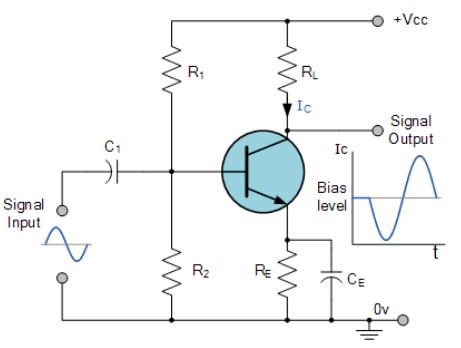
\includegraphics[width=8cm]{Imagenes/potencia_bjt.jpg}
    \caption{Transistor BTJ en configuración Emisor Común para amplificación de CA}
    \label{fig:potencia}
\end{figure}

\subparagraph{Amplificador de potencia clase B o Push and Pull:}

Los amplificadores de Clase B usan dos o más transistores polarizados de tal forma que cada transistor solo conduce durante un medio ciclo (realmente, "casi" medio ciclo) de la onda de entrada. Tienen un rendimiento muy superior a los de Clase A y su diseño no es muy complicado, pero sus aplicaciones se limitan enormemente debido a una característica su propio diseño: una distorsión llamada de "cruce por cero". Aún así, se utilizan incluso en amplificadores que no requieran buena fidelidad y sí facilidad de diseño y rendimiento, como los amplificadores de bocinas y megáfonos de mano.

Para mejorar la eficiencia de potencia total del amplificador de clase A previo, reduciendo la potencia desperdiciada en forma de calor, es posible diseñar el circuito amplificador de potencia con dos transistores en su etapa de salida, produciendo lo que comúnmente se denomina amplificador de clase B; también conocido como configuración de amplificador Push-Pull (empuja-tira en español). Para construir este tipo de amplificador se utilizan necesariamente transistores denominados "complementarios", es decir, de las mismas características eléctricas pero con distintas uniones P-N: si uno es del tipo NPN, el otro ha de ser igual pero de tipo PNP.

\begin{figure}[H]
    \centering
    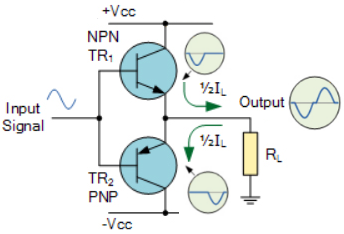
\includegraphics[width=8cm]{Imagenes/clase_b.png}
    \caption{transistores complementarios BJT en funcionamiento clase B, configuración Push-Pull}
    \label{fig:clase_b}
\end{figure}


Los amplificadores Push-Pull utilizan transistores complementarios de potencia, que reciben la misma señal de entrada que es igual en magnitud, pero en fase opuesta entre sí. Esto da lugar a que un transistor solamente amplifica la mitad o 180º del ciclo de la onda de entrada; mientras que el otro transistor amplifica la otra mitad o restante 180º del ciclo de onda de entrada.

Conjuntamente, estas “dos mitades” amplificadas cada una por un transistor, "excitan" o "atacan" la carga o resistencia de salida, dando lugar en ella a la señal completa amplificada.

Por consiguiente, el ángulo de conducción para este tipo de circuito amplificador es escasamente inferior a 180º o $50\%$ de la señal de entrada (para cada transistor). Este efecto de empujar y tirar de los semi ciclos alternos por los transistores da a este tipo de circuito su divertido nombre "push-pull", pero en general se lo conoce como el amplificador de clase B.

Realmente los transistores en un amplificador de clase B no llegan al conducir el $50\%$, ya que ambos necesitan tener una polarización al menos de 0.65 V Emisor-Base para empezar a conducir y amplificar. Esto supone que de la señal de entrada, en los primeros 0.65 V. (positivos y negativos), la señal de salida va a estar a "0". Y sólo cuando en la entrada se superen los 0.65 V. E-B podrá empezar a amplificar la salida. Esto, al final, produce inevitablemente una falta de amplificación en torno a los valores cercanos a "0" V. denominada "distorsión de paso por cero" o "distorsión de cruce", característica de los amplificadores en Clase B.

\begin{figure}[H]
    \centering
    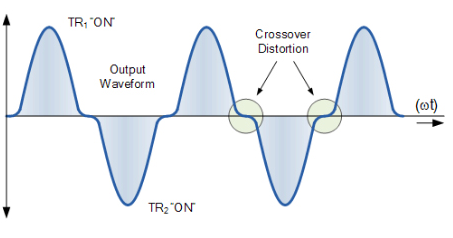
\includegraphics[width=10cm]{Imagenes/crossover.png}
    \caption{formas de señal de saldia debida a la "distorsión de cruce"    o     "de paso por 0" en un amplificador Clase B, Push-Pull}
    \label{fig:crossover}
\end{figure}

\subparagraph{Amplificador de potencia clase AB:}

Un amplificador de clase AB está polarizado de modo que la corriente de salida fluye durante menos de un ciclo completo de la forma de onda de entrada pero más de medio ciclo. La implementación de los amplificadores de Clase AB es muy similar a las configuraciones de Clase B estándar en que utiliza dos transistores de conmutación como parte de una etapa de salida complementaria con cada transistor conduciendo en semi-ciclos opuestos de la forma de onda de entrada antes de combinarse en la carga.

Por lo tanto, al permitir que ambos transistores de conmutación conduzcan corriente al mismo tiempo durante un período muy corto, la forma de onda de salida durante el período de cruce cero se puede suavizar sustancialmente reduciendo la distorsión de cruce asociada con el diseño del amplificador de clase B. Entonces el ángulo de conducción es mayor de 180° pero mucho menor de 360°.

\begin{figure}[H]
    \centering
    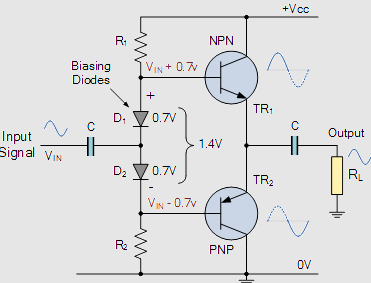
\includegraphics[width=10cm]{Imagenes/clase_ab.png}
    \caption{Esquemático de un amplificador clase AB, polarizado por diodos }
    \label{fig:clase_ab}
\end{figure}

Una configuración de amplificador de clase AB es más eficiente que un amplificador de clase A pero un poco menos eficiente que la de un clase B debido a la pequeña corriente de reposo necesaria para polarizar los transistores justo por encima del límite. Sin embargo, el uso de polarización incorrecta puede causar picos de distorsión cruzada que producen una peor condición.

Dicho esto, los amplificadores de clase AB son uno de los diseños de amplificadores de potencia de audio más preferidos debido a su combinación de una eficiencia razonablemente buena y una salida de alta calidad, ya que tienen una baja distorsión de cruce y una alta linealidad similar al diseño de amplificador de clase A.

\subparagraph{Amplificador de potencia clase C:}

Los amplificadores de potencia en clase C parten de la premisa siguiente: no se trata de amplificar con calidad la señal de entrada, se trata simplemente de amplificar la señal de entrada de modo que a la salida se obtenga el máximo rendimiento posible pero sólo para un rango de frecuencias muy reducido, en torno a una de "resonancia".

Son amplificadores que desde luego no sirven para señales de audio, por la distorsión. Su campo de aplicación está en las telecomunicaciones, en radiofrecuencia, F, donde se requiere un incremento en el nivel de potencia y no se requiere linealidad entre la tensión de entrada y tensión de salida. Los amplificadores Clase C pueden ser modulados en amplitud para amplificar una portadora modulada en frecuencia.

\begin{figure}[H]
    \centering
    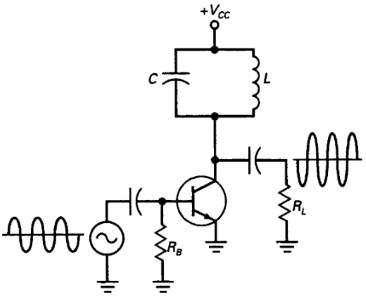
\includegraphics[width=7cm]{Imagenes/amplificador resonante01.png}
    \caption{etapa amplificadora a transistor BJT con circuito tanque resonante }
    \label{fig:clase_c}
\end{figure}

Este tipo de amplificadores se reconoce porque tienen, en lugar de la resistencia de colector típica, un "circuito tanque" formado por un condensador y bobina diseñados para que en un estrecho margen de frecuencias entren en sintonía -por lo que también se le llama "circuito resonante"-y, modificando la impedancia del circuito L-C produzcan la conducción del transistor. Es por eso que a este tipo de circuitos les llama amplificadores "resonantes" o "sintonizados".

En torno a la frecuencia de resonancia, estos amplificadores obtienen una ganancia alta; fuera de esta frecuencia, la amplificación es muy reducida y el consumo es mínimo.


\begin{figure}[H]
    \centering
    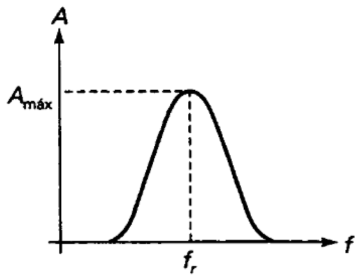
\includegraphics[width=7cm]{Imagenes/amplificador resonante02.png}
    \caption{etapa amplificadora a transistor BJT con circuito tanque resonante }
    \label{fig:campana de gauss}
\end{figure}

\subsubsection{Amplificadores de varias etapas}

La conexión más utilizada para amplificadores de varias etapas:

\paragraph{\textbf{Conexión en cascada}}

\begin{figure}[H]
    \centering
    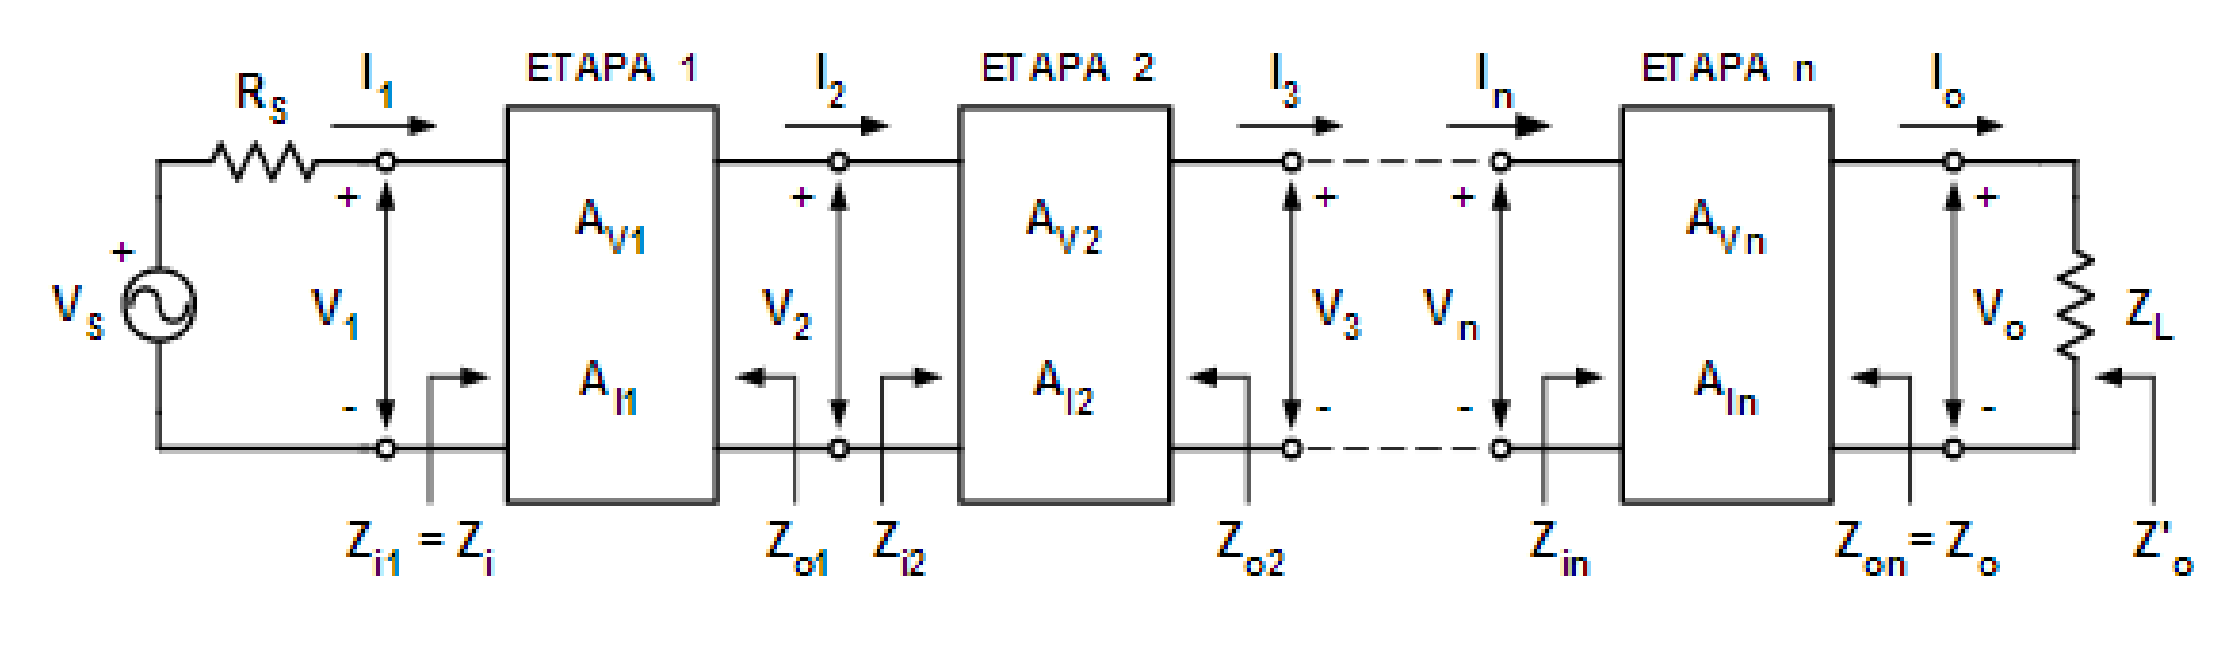
\includegraphics[width=15cm]{Imagenes/amp_base.png}
    \caption{Conexión en cascada de varios amplificadores}
    \label{fig:cascada}
\end{figure}

Hay influencias de una etapa sobre otra, la señal de salida de cada etapa se aplica como señal de entrada de la siguiente.

Las ganancias de tensión de cada etapa y sus impedancias teniendo en cuenta lo siguiente, serán:
\begin{gather}
    A_v= A_{v1}A_{v2}...A_{vn}
    \label{eqn:avt}
\end{gather}

\begin{align*}
     & \text{Impedancia de entrada} &  & Z_in= Z_n        \\
     & \text{Impedancia de salida}  &  & Z_o= Z_{On}      \\
     &                              &  & Z'_o= Z_{L}||Z_o
\end{align*}

Nosotros nos centraremos en los amplificadores de alterna, hay varios tipos de acoplamientos entre etapas, aquí nos centraremos en el acoplamiento RC.

El acoplamiento entre etapas es mediante un condensador. Como se indico anteriormente sobre los condensadores de acople y desacople.

\newpage

\subsection{Respuesta en frecuencia}

A respuesta en frecuencia de un amplificador operacional en lazo cerrado o lazo abierto se define como el límite de alta frecuencia y el límite de baja frecuencia. En estos límites, la ganancia de voltaje se reduce un 0.707 del valor máximo de voltaje, en el rango de frecuencia útil.
El ancho de banda para pequeña señal es la diferencia entre el límite de alta frecuencia y el límite de baja frecuencia. Además se debe agregar que:

\begin{itemize}
    \item \textbf{Para frecuencias medias}, los condensadores de acople y desacople se comportan como un cable, es decir, un cortocircuito.
    \item \textbf{Para frecuencias altas}, las limitaciones en frecuencia de los dispositivos activos condicionan 1a frecuencia máxima de operación del amplificador.
    \item \textbf{Para frecuencias bajas}, el efecto de los condensadores de acoplo y desacoplo es importante.
\end{itemize}

\subsubsection{Análisis de respuesta en frecuencia}

\begin{itemize}
    \item \textbf{Frecuencias bajas:} Se toma en cuenta el condensador que se va a estudiar en bajas frecuencias, siendo estos los de acople, desacople y bypass. Al escoger el condensador, ese se reemplaza por una fuente de prueba y los demás capacitores se cortocircuitan y los de alta frecuencia son un abierto. Así, se puede hallar la impedancia equivalente. Se hace uso de la ecuación \ref{eqn:wl}.

          \begin{equation}
              w_{p_n}=\dfrac{1}{C_nZ_{eq}}
              \label{eqn:wl}
          \end{equation}

    \item \textbf{Frecuencias altas:} Se toma en cuenta los capacitores que estén conectados entre base y emisor o base y colector, con un valor de capacitancia bastante bajo, cercano a los $\si{pF}$. Se aplica el teorema de miller, que es la ecuación \ref{eqn:C_eq} y su frecuencia de corte superior siendo la ecuación \ref{eqn:wh}.

          \begin{equation}
              w_{H}=\dfrac{1}{C_{eq}Z_{in}}
              \label{eqn:wh}
          \end{equation}

    \item \textbf{Frecuencia de corte superior total}
          \begin{equation}
              w_t=\beta \cdot f_H
              \label{eqn:wt}
          \end{equation}
\end{itemize}



\subsection{Realimentación en un amplificador}

La realimentación consiste e11 combinar una muestra de la señal de salida del amplificador con la señal de entrada, de modo tal que se modifican las características generales del sistema. Puede ser positiva o negativa.

\subsubsection{Realimentación negativa}

La realimentación es negativa cuando el valor de la señal de salida es menor que sin la realimentación. Para ello, la serial de salida que se toma como muestra es aplicada opuesta en fase a la serial de entrada.

La realimentación negativa disminuye la ganancia del amplificador y a pesar de ello, la inmensa mayoría de los amplificadores utilizan esta variante de realimentación debido a las muchas ventajas que se obtienen con la aplicación de este principio, tales como el aumento
de la estabilidad y el ancho de banda, 1a disminución de las distorsiones de frecuencia y de no linealidad así como del ruido y el cambio en las resistencias de entrada y salida. Todo esto incrementa notablemente la calidad y versatilidad de los amplificadores.

Los cambios provocados por el envejecimiento de los componentes y dispositivos, su reemplazo u otras causas, las variaciones de temperatura, etcétera, se reflejan en las alteraciones que puede sufrir la ganancia de un amplificador con relación a su valor original. Tales
alteraciones son de hecho reducidas con la realimentación negativa, a tal extremo que su ganancia puede llegar a depender solamente de las características de la red de realimentación, cuando la ganancia de lazo es mucho mayor que la unidad.


\subsubsection{frecuencia de corte inferior en realimentación no inversora}
\begin{equation}
    w_{L_{fb}}=\dfrac{w_L}{A_{fb}}=\dfrac{w_L}{1+\dfrac{R_f}{R_s}}
    \label{eqn:wlfb}
\end{equation}
\subsubsection{frecuencia de corte superior en realimentación no inversora}
\begin{equation}
    w_{H_{fb}}=w_H(A_{fb})=w_L(1+\dfrac{R_f}{R_s})
    \label{eqn:whfb}
\end{equation}

\subsubsection{Ganancia en retroalimentación de un no inversor}
\begin{equation}
    A_{fb}=1+\dfrac{R_f}{R_s}
    \label{eqn:afb}
\end{equation}


\subsubsection{Impedancias de entrada en realimentación negativa o degenerativa}
\begin{equation}
    Z_{in}=Z_d\left(1 +\dfrac{A_{fm}}{A_{fb}}\right)
    \label{eqn:zinfb}
\end{equation}
\subsubsection{Impedancias de salida en realimentación negativa o degenerativa}
\begin{equation}
    Z_{o}=\left(\dfrac{Z_o}{\dfrac{A_{fm}}{A_{fb}}}\right)
    \label{eqn:zofb}
\end{equation}
\subsubsection{Realimentación positiva}

La realimentación es positiva cuando el valor de la señal de salida es mayor que sin la realimentación. Esto se logra cuando la señal de salida que se toma como muestra es
aplicada en fase con la señal de entrada.

El resultado de la realimentación positiva es contrario a la realimentación negativa, es decir se incrementa el ruido, la ganancia y la distorsión, disminuyendo el ancho de banda y la estabilidad, por lo cual este efecto no es aconsejable para los amplificadores, sin embargo, puede ser aprovechado con gran eficacia en los circuitos osciladores.

\subsection{Método de amplificador desvanecido}

El método consiste en añadir una ganancia adicional variable a la señal recibida, dependiendo de la calidad de la señal, para compensar la atenuación y mejorar la relación señal—ruido. Esta ganancia adicional se calcula en función de la retroalimentación recibida de la señal de error, que se obtiene comparando la señal recibida con la señal transmitida originalmente.

El Amplificador Desvanecido puede ser implementado de varias maneras, incluyendo la retroalimentación de la señal de en un circuito de control de ganancia, o utilizando
técnicas de procesamiento digital de señales para ajustar la ganancia en tiempo real.

Este método es particularmente útil en sistemas de comunicación inalámbrica de alta frecuencia, como los sistemas de comunicación móvil, donde la atenuación de la señal debido a la propagación en el medio ambiente puede ser significativa y afectar la calidad de la señal
recibida.

\subsection{Método de Blackman}

Es una técnica utilizada para calcular la impedancia de entrada de un amplificador.Esta técnica se basa en la medición de la tensión de entrada y corriente de entrada del
amplificador, y en el uso de una red de resistencias y capacitores para modelar la impedancia
de entrada del amplificador.

El método de Blackman utiliza una red de dos resistencias y un capacitor, conectados en serie con la entrada del amplificador. La tensión de entrada se mide a través de una de las resistencias, mientras que la corriente de entrada se mide a través de la otra resistencia.

A partir de estas mediciones, se puede calcular la impedancia de entrada del amplificador utilizando la ley de Ohm y la ley de Kirchhoff.

La ventaja del método de Blackman es que permite obtener una medida precisa de la impedancia de entrada del amplificador en una amplia gama de frecuencias. Además, esta
técnica es relativamente sencilla y económica de implementar, lo que la hace adecuada para su uso en aplicaciones practicas.

Sin embargo, es importante tener en cuenta que el método de Blackman asume que la impedancia de entrada del amplificador es constante en toda la gama de frecuencias de
interés, lo cual puede no ser cierto en algunos casos.

\subsection{Formula de propagación de incertidumbres}

Para calcular la incertidumbre en un resultado calculado indirectamente, como \( V_{CE} = V_C - V_E \), puedes utilizar la fórmula de propagación de incertidumbres. Esta fórmula se aplica cuando tienes dos o más cantidades medidas y deseas determinar la incertidumbre en una cantidad derivada a partir de ellas. La fórmula general es:

\[ \Delta Q = \sqrt{\left(\frac{\partial Q}{\partial A} \Delta A\right)^2 + \left(\frac{\partial Q}{\partial B} \Delta B\right)^2 + \ldots} \]

Donde:
- \( Q \) es la cantidad derivada (en este caso, \( V_{CE} \)),
- \( A, B, \ldots \) son las cantidades medidas (en este caso, \( V_C \) y \( V_E \)),
- \( \Delta A, \Delta B, \ldots \) son las incertidumbres asociadas a las cantidades medidas, y
- \( \frac{\partial Q}{\partial A}, \frac{\partial Q}{\partial B}, \ldots \) son las derivadas parciales de \( Q \) con respecto a \( A, B, \ldots \).

En este caso, como \( V_{CE} = V_C - V_E \), las derivadas parciales son simples:

\[ \frac{\partial V_{CE}}{\partial V_C} = 1, \quad \frac{\partial V_{CE}}{\partial V_E} = -1 \]

Entonces, la fórmula para la incertidumbre en \( V_{CE} \) sería:

\[ \Delta V_{CE} = \sqrt{\left(\Delta V_C\right)^2 + \left(\Delta V_E\right)^2} \]

Sustituyendo los valores dados:

\[ \Delta V_{CE} = \sqrt{(0.1)^2 + (0.02)^2} \]

\[ \Delta V_{CE} = \sqrt{0.01 + 0.0004} \]

\[ \Delta V_{CE} \approx \sqrt{0.0104} \]

\[ \Delta V_{CE} \approx 0.102 \volt \]

Entonces, la incertidumbre en \( V_{CE} \) es aproximadamente \( \pm 0.102 \volt \). Puedes informar el resultado como \( V_{CE} = 1.06 \pm 0.102 \volt \).

\subsection{Error Porcentual}

Porcentaje de error (\% de error), también conocido como porcentaje de error, es una medida de cuánto un valor difiere del valor esperado. Puede usarse para determinar qué tan lejos está un valor esperado de otro valor, pero a menudo se usa en el contexto de experimentos científicos.

Se puede expresar en la siguiente ecuación:

\begin{equation}
    E_r =\dfrac{|Valor_{experimental}-Valor_{teorico}|}{Valor_{teorico}} \cdot  100
    \label{eqn:error}
\end{equation}

\subsection{Impedancia de entrada/diferencial (medición indirecta)}

La siguiente ecuación se lleva a cabo debido a un divisor de tensión realizado de la siguiente manera:

\begin{figure}[H]
    \centering
    \begin{circuitikz}[transform shape,scale=1]

  \draw (2.25,-2.25) to[short,-*] (2.25,-2.25) coordinate (X0);
  \def\OpAmpsopamp(#1)#2#3{%
    \begin{scope}[#1,transform canvas={scale=1}]
      \draw (0.0,0.25) -- (1.0,-0.25);
      \draw (0.0,-0.75) -- (1.0,-0.25);
      \draw (0.0,0.25) -- (0.0,-0.75);
      \draw (0.0625,0.0) -- (0.1875,0.0);
      \draw (0.0625,-0.5) -- (0.1875,-0.5);
      \draw (0.125,-0.5625) -- (0.125,-0.4375);
      \draw (0.5,0.25) coordinate (#2 text);
      \draw (0.0,0.0) coordinate (#2 X0);
      \draw (0.0,-0.5) coordinate (#2 X1);
      \draw (1.0,-0.25) coordinate (#2 X2);
    \end{scope}
    \draw (#2 text) node[right] {#3};
  }
  \draw (2.25,-3.5) node[ground] {} ;
  \node[right] at (-2.0,-2.25) {Vg} ;
  \node[right] at (2,-2.0) {Vi} ;
  \node[right] at (5.5,-2.5) {Vo} ;
  \OpAmpsopamp (shift={(3.5,-2.25)},rotate=0  ) {B0} {Amp. Op};
  \draw (X0) to[R,l=Rp] (-0.5,-2.25) ;
  \draw (B0 X0) to[short,-] (X0) ;
  \draw (5.5,-2.5) to[short,-] (5.0,-2.5) ;
  \draw (B0 X1) to[short,-] (2.25,-2.75) ;
  \draw (2.25,-3.5) to[short,-] (2.25,-2.75) ;
  \draw (-0.5,-2.25) to[short,-] (-1.0,-2.25) ;
  \draw (5.0,-2.5) to[short,-] (B0 X2) ;

\end{circuitikz}
    \caption{Circuito simplificado de un amplificador para hallar su impedancia de entrada}
    \label{fig:zin_amp}
\end{figure}

\begin{gather}
    V_i=V_g \, \dfrac{Z_{d}}{Z_{d}+R_p} \nonumber \\[0.2cm]
    V_iZ_{d}+V_iR_p = V_gZ_{d} \nonumber \\[0.2cm]
    V_gZ_{d} - V_iZ_{d} = V_iR_p  \nonumber \\[0.2cm]
    Z_{d} = V_i \dfrac{R_p}{V_g-V_i}  \label{eqn:zin}
\end{gather}

\subsection{Impedancia de entrada/modo Común (medición indirecta)}

Se visualiza el modelo del amplificador para sus impedancias de entrada en modo común, donde se usará la siguiente ecuación:

\begin{gather}
    V_i=V_g \,\dfrac{Z_{c}}{2} \dfrac{1}{\dfrac{Z_{c}}{2}+R_p} \nonumber \\[0.2cm]
    V_i=V_g \, \dfrac{Z_{c}}{2} \dfrac{1}{\dfrac{Z_{c}+2R_p}{2}} \nonumber \\[0.2cm]
    V_iZ_{c}+2V_iR_p = V_gZ_{c} \nonumber \\[0.2cm]
    V_gZ_{c} - V_iZ_{c} = 2V_iR_p  \nonumber \\[0.2cm]
    Z_{c} = 2V_i \dfrac{R_p}{V_g-V_i}  \label{eqn:zc}
\end{gather}

\subsection{Impedancia de salida (medición indirecta)}

La siguiente ecuación, al igual que la impedancia de entrada se lleva a cabo con un divisor de tensión, como se verá a continuación:

\begin{figure}[H]
    \centering 
\ctikzset{tripoles/mos style/arrows} 
\begin{circuitikz}[transform shape,scale=1] 
 
\def\OpAmpsopamp(#1)#2#3{%
  \begin{scope}[#1,transform canvas={scale=1}]
  \draw (0.0,0.25) -- (1.0,-0.25);
  \draw (0.0,-0.75) -- (1.0,-0.25);
  \draw (0.0,0.25) -- (0.0,-0.75);
  \draw (0.0625,0.0) -- (0.1875,0.0);
  \draw (0.0625,-0.5) -- (0.1875,-0.5);
  \draw (0.125,-0.5625) -- (0.125,-0.4375);
  \draw (0.5,0.25) coordinate (#2 text);
  \draw (0.0,0.0) coordinate (#2 X0);
  \draw (0.0,-0.5) coordinate (#2 X1);
  \draw (1.0,-0.25) coordinate (#2 X2);
  \end{scope}
  \draw (#2 text) node[right] {#3};
}
\draw (2.25,-3.5) node[ground] {} ;
\node[right] at (5.5,-2.5) {Vosc} ;
\node[right] at (1.50,-2.25) {Vi} ;
\OpAmpsopamp (shift={(3.5,-2.25)},rotate=0  ) {B0} {AmpOp};
\draw (B0 X0) to[short,-] (2.875,-2.25) ;
\draw (5.5,-2.5) to[short,-] (5.0,-2.5) ;
\draw (B0 X1) to[short,-] (2.25,-2.75) ;
\draw (2.25,-3.5) to[short,-] (2.25,-2.75) ;
\draw (2.875,-2.25) to[short,-] (2.25,-2.25) ;
\draw (5.0,-2.5) to[short,-] (B0 X2) ;

\end{circuitikz}
    \caption{Circuito simplificado de un amplificador para medir su voltaje sin carga, medida para hallar su impedancia de salida}
    \label{fig:zout_amp1}
\end{figure}

\begin{figure}[H]
    \centering
    \ctikzset{tripoles/mos style/arrows} 
\begin{circuitikz}[transform shape,scale=1] 
 
\draw (5.0,-2.5) to[short,-*] (5.0,-2.5) coordinate (X0);
\def\OpAmpsopamp(#1)#2#3{%
  \begin{scope}[#1,transform canvas={scale=1}]
  \draw (0.0,0.25) -- (1.0,-0.25);
  \draw (0.0,-0.75) -- (1.0,-0.25);
  \draw (0.0,0.25) -- (0.0,-0.75);
  \draw (0.0625,0.0) -- (0.1875,0.0);
  \draw (0.0625,-0.5) -- (0.1875,-0.5);
  \draw (0.125,-0.5625) -- (0.125,-0.4375);
  \draw (0.5,0.25) coordinate (#2 text);
  \draw (0.0,0.0) coordinate (#2 X0);
  \draw (0.0,-0.5) coordinate (#2 X1);
  \draw (1.0,-0.25) coordinate (#2 X2);
  \end{scope}
  \draw (#2 text) node[right] {#3};
}
\draw (2.25,-3.5) node[ground] {} ;
\node[right] at (5.5,-2.5) {Vocc} ;
\node[right] at (1.50,-2.25) {Vi} ;
\draw (5.0,-3.75) node[ground] {} ;
\OpAmpsopamp (shift={(3.5,-2.25)},rotate=0  ) {B0} {AmpOp};
\draw (X0) to[R,l=Rp] (5.0,-3.75) ;
\draw (B0 X0) to[short,-] (2.875,-2.25) ;
\draw (X0) to[short,-] (B0 X2) ;
\draw (5.5,-2.5) to[short,-] (X0) ;
\draw (B0 X1) to[short,-] (2.25,-2.75) ;
\draw (2.25,-3.5) to[short,-] (2.25,-2.75) ;
\draw (2.875,-2.25) to[short,-] (2.25,-2.25) ;

\end{circuitikz}
    \caption{Circuito simplificado de un amplificador para medir su voltaje con carga, medida para hallar su impedancia de salida}
    \label{fig:zout_amp2}
\end{figure}

Como se observa en la figura \ref{fig:zout_amp1} y \ref{fig:zout_amp2}, luego de realizar esas medidas se realiza un divisor de tensión que permite la medición de su impedancia.

\begin{gather}
    V_{occ}=\dfrac{V_{oscR_p}}{R_p + Z_o} \nonumber \\[0.2cm]
    Z_oV_{occ} + V_{occ}R_p=V_{osc}R_p \nonumber \\[0.2cm]
    Z_o= \dfrac{V_{osc}R_p - V_{occ}R_p}{V_{occ}} \label{eqn:zo}
\end{gather}


\subsection{Uso de PPM en la Incertidumbre de la Medición del Intervalo de Tiempo en un Osciloscopio}

En el ámbito de la electrónica y la instrumentación, la precisión y la exactitud de las mediciones son cruciales. Los osciloscopios, herramientas esenciales en la medición de señales eléctricas, requieren una comprensión detallada de sus especificaciones para asegurar resultados confiables. Una de las métricas importantes en estos dispositivos es la incertidumbre de la medición del intervalo de tiempo, donde el concepto de partes por millón (ppm) juega un papel significativo.

\subsubsection{Concepto de PPM (Partes por Millón)}

PPM es una unidad de medida que expresa una proporción como una fracción de un millón. Es comúnmente utilizada en campos donde se requieren mediciones extremadamente precisas, como en la electrónica, para representar pequeñas variaciones o errores relativos en una cantidad medida. En el contexto de un osciloscopio, ppm se emplea para cuantificar la exactitud del intervalo de tiempo medido, relacionando el error relativo con la lectura.

Matemáticamente, 1 ppm se define como:

\[
    1 \, \text{ppm} = \frac{1}{1,000,000} = 10^{-6}
\]

\subsubsection{Incertidumbre de la Medición del Intervalo de Tiempo}

La incertidumbre en la medición del intervalo de tiempo de un osciloscopio es la desviación esperada de la medida real debido a las limitaciones del dispositivo. Esta incertidumbre se compone de varios factores, incluyendo el intervalo de muestreo, la resolución del dispositivo, y un componente proporcional a la lectura expresado en ppm.

En el manual de un osciloscopio típico, la incertidumbre de la medición del intervalo de tiempo (\(\Delta T\)) se especifica como:

\[
    \Delta T = \pm \left( \text{intervalo de muestreo} + 50 \text{ ppm} \times \text{lectura} + 0.6 \text{ ns} \right)
\]

\subsubsection{Desglose de la Fórmula}

\begin{enumerate}
    \item \textbf{Intervalo de Muestreo}

          Es el tiempo entre dos muestras consecutivas que toma el osciloscopio. A menor intervalo de muestreo, mayor es la precisión temporal del dispositivo.

    \item \textbf{50 ppm \(\times\) Lectura}

          Este término indica que el error relativo es proporcional a la lectura del intervalo de tiempo. La constante de 50 ppm refleja la precisión del osciloscopio en términos de ppm. Para convertir 50 ppm a una fracción decimal:

          \[
              50 \, \text{ppm} = 50 \times 10^{-6} = 0.00005
          \]

          Por lo tanto, si la lectura es de 100 ns, el error debido a este término sería:

          \[
              0.00005 \times 100 \, \text{ns} = 0.005 \, \text{ns}
          \]

    \item 0.6 ns

          Un componente fijo de la incertidumbre que representa errores sistemáticos adicionales en la medición.

\end{enumerate}

\subsubsection{Importancia en Aplicaciones Electrónicas}

Comprender la incertidumbre de la medición es esencial para ingenieros y técnicos que dependen de los osciloscopios para diseñar, probar y verificar circuitos electrónicos. La especificación en ppm permite evaluar y comparar la precisión de diferentes osciloscopios, asegurando que las mediciones sean suficientemente precisas para las aplicaciones específicas.

\newpage


%Objetivos generales y Específicos

\section{Objetivo General y Específico}

    \subsection*{Parte 1: Aplicaciones de las Topologías Clásicas}
    
        \subsubsection*{Objetivo General:}
        Reconocer las ventajas del uso del concepto de amplificadores operacionales en el diseño e implementación de sistemas analógicos.
        
        \subsubsection*{Objetivos Específicos:}
        \begin{enumerate}
            \item Conocer las desviaciones de las implementaciones comerciales del amplificador operacional ideal.
            \item Reconocer las ventajas del uso de amplificadores operacionales en sistemas de procesamiento de señal, en comparación con sistemas implementados con componentes discretos.
        \end{enumerate}
    
    \subsection*{Parte 2: Amplificador Operacional Real}
    
        \subsubsection*{Objetivo General:}
        Reconocer las ventajas del uso del concepto de amplificadores operacionales en el diseño e implementación de sistemas analógicos.
        
        \subsubsection*{Objetivos Específicos:}
        \begin{enumerate}
            \item Conocer las desviaciones de las implementaciones comerciales del amplificador operacional ideal.
            \item Reconocer los efectos de las imperfecciones de los amplificadores operacionales y aplicar técnicas para corrección de estos efectos.
        \end{enumerate}
    
    \subsection*{Parte 3: Filtros Activos}
    
        \subsubsection*{Objetivo General:}
        Reconocer las ventajas del uso del concepto de amplificadores operacionales en el diseño e implementación de sistemas analógicos.
        
        \subsubsection*{Objetivos Específicos:}
        \begin{enumerate}
            \item Reconocer los efectos que produce la aplicación de filtros pasa bajos, pasa banda y pasa altos en distintas señales.
        \end{enumerate}
    
    \subsection*{Parte 4: Fuentes Lineales y Reguladores Monolíticos}
    
        \subsubsection*{Objetivo General:}
        Reconocer, comprender y utilizar algunas de las aplicaciones del amplificador operacional más frecuentemente utilizadas.
        
        \subsubsection*{Objetivos Específicos:}
        \begin{enumerate}
            \item Analizar el funcionamiento de topologías de fuentes reguladas lineales series basadas en reguladores monolíticos comerciales fijos y variables.
        \end{enumerate}
    

\newpage

s%Metodología
\section{Metodología}

\begin{figure}[H]
  \centering
  \adjustbox{width = 15cm}{
\ctikzsubcircuitdef{power}{in 1,in 3,in 2}{
    coordinate (#1-in 1) to[R,l=$R_{17}$,*-*] ++(0,-4.50) coordinate (#1-in 3)
    (#1-in 3) --++(1.5,0) node[npn,anchor=B](Q5){$Q_{5}$}
    (#1-in 1) -| (Q5.C)
    (Q5.E) to[R,l=$R_{13}$,*-*] ++(0,-2) coordinate (A) to[C,l_=$C_{5}$] ++(2,0) to[R,l=$R_{L}$,*-*] ++(0,-2) node[vee](VEE){$-10\volt$}
    (A) to[R,l=$R_{14}$,*-*] ++(0,-2) node[pnp, anchor=E](Q6){$Q_{6}$}
    (#1-in 3) --++(0,-1.5) coordinate(A1) --++(1,0) --++ (0,-0.5) node[npn,anchor=C](Q4){$Q_{4}$}
    (Q4.E) --++(0,-0.5) --++(-1,0) coordinate(A2)
    (A1) --++(-1,0) --++(0,-0.71) node[potentiometershape, rotate=-90,anchor=west,label=south west:$R_{V1}$, font=\large](P){}
    (P.wiper) -| (Q4.B)
    (P.east) --++(0,-0.71) -| (A2)
    (A2) --++(0,-1.5) coordinate (A3) -| (Q6.B)
    (A3) to[R,l=$R_{12}$,*-] ++(0,-2) coordinate (#1-in 2)
    (Q6.C) --++(0,-1.5) -| (#1-in 2)
}

\ctikzsubcircuitdef{driver}{in 1, in 2, in 3, out 1, out 2, out 3}{
coordinate (#1-in 3) --++(0.5,0) node[pnp, anchor=B](Q3){$Q_{3}$}
(#1-in 3) to[R,l=$R_{15}$,*-*] ++(0,3.23) coordinate (#1-in 1) ++(0,0) node[vcc](VCC){$10\volt$}
(#1-in 3) --++(0,-1.27) coordinate (B1) to[R,l=$R_{10}$,*-*] ++(0,-7.81) coordinate (#1-in 2) ++(0,0) node[vee](VEE){$-10\volt$}
(Q3.E) to[R,l=$R_{11}$,*-*] ++(0,2.46) coordinate (B3)
(Q3.E) --++(1.5,0) to[C,l=$C_{6}$,*-*] ++(0,2.46) coordinate (#1-out 1) --(B3) -| (#1-in 1)
(Q3.C) --++(0,-0.5) coordinate (#1-out 3) to[R,l=$R_{16}$,*-*] ++(0,-7.81) coordinate (#1-out 2) -| (#1-in 2)
(B1) --++(0.4,0) to[C,l=$C_{4}$] ++(0.5,0) -| (#1-out 3)
}

\ctikzsubcircuitdef{differential}{in 1,out 1, out 2,out 3}{
    coordinate (#1-in 1) --++(1,0) node[npn, anchor=B](Q1){$Q_{1}$}
    (Q1.C) --++(0,1) coordinate (#1-out 3) to[R,l=$R_{3}$,*-] ++(0,2) coordinate (C)
    (Q1.E) to[R,l=$R_{4}$,*-] ++(0,-6) coordinate (C2)
    (#1-in 1) to[R,l=$R_{1}$,*-*] ++(0,5) -| (C)
    (#1-in 1) to[R,l=$R_{2}$,*-*] ++(0,-7.31) -| (C2)
    (Q1.E) to[R,l_=$R_{5}$,*-*] ++(2.5,0) coordinate (C3) to[R,l=$R_{7}$,*-*] ++(0,-6.54) coordinate (C6) -| (C2)
    (C3) node[npn,xscale=-1, anchor=E,label=left:$Q_{2}$](Q2){} ++(0,1.5)
    (Q2.C) to[R,l=$R_{6}$,*-*] ++(0,4.23) coordinate (C4) -| (C)
    (Q2.B) --++(0.5,0) coordinate (C5) to[R,l=$R_{9}$,*-*] ++(0,-7.31) coordinate (#1-out 2) -| (C6)
    (C5) to[R,l=$R_{8}$,*-*] ++(0,5) coordinate (#1-out 1) -| (C4)
    (C5) --++(1,0) to[C,l=$C_{3}$,*-*] ++(0,-2) node[vee](VEE){$-10\volt$}
}
\ctikzsubcircuitdef{universall}{in 1,out 3}{
    coordinate (#1-in 1) --++(1,0) node[npn, anchor=B](Q1){$Q_{1}$}
    (Q1.C) --++(0,1) coordinate (#1-out 3) to[R,l=$R_{3}$,*-] ++(0,2) coordinate (C)
    (Q1.E) to[R,l=$R_{4}$,*-] ++(0,-6) coordinate (C2)
    (#1-in 1) to[R,l=$R_{1}$,*-*] ++(0,5) -| (C)
    (#1-in 1) to[R,l=$R_{2}$,*-*] ++(0,-7.31) -| (C2) (Q1.E) 
}

\ctikzsubcircuitactivate{universall}
\ctikzsubcircuitactivate{power}
\ctikzsubcircuitactivate{driver}
\ctikzsubcircuitactivate{differential}

\begin{circuitikz}\draw
    (0,0)\driver{driv}{out 3} to[C,l=$C_{7}$,*-*]++(3,0) \power{power}{in 3}
    (driv-out 1) -| (power-in 1)
    (driv-out 2) -| (power-in 2)
    (driv-in 3) to[C,l=$C_{2}$,*-*]++(-6,0) \differential{dif}{out 3}
    (driv-in 1) -| (dif-out 1)
    (driv-in 2) -| (dif-out 2)
    (dif-in 1) to[C,l=$C_{1}$,*-*] ++(-2,0) to[short,-o, label=$V_{in}$] ++(-0.5,0)
;\end{circuitikz}
}
  \caption{Diagrama Esquemático del Amplificador Base}
  \label{fig:amplificador_base}
\end{figure}

\subsection{Parte 1. Amplificador de potencia}
\begin{enumerate}
  \item \textbf{Identifique la etapa de Potencia (EP) en el amplificador base.}

        \begin{figure}[H]
          \centering
          \adjustbox{width = 3cm}{
\begin{circuitikz}\draw
   \power{power}{in 3}
    (driv-out 1) -| (power-in 1) ++(0,0) node[vcc](VCC){$10\volt$}
    (driv-out 2) -| (power-in 2) ++(0,-0.25) node[vee](VEE){$-10\volt$}
    (0,0) to[C,l=$C_{7}$,*-*]++(-2,0) 
;\end{circuitikz}}
          \caption{Diagrama Esquemático de la  etapa de potencia}
          \label{fig:amplificador_potencia}
        \end{figure}

        La etapa de Potencia es la que se observa en la figura \ref{fig:amplificador_potencia}, que se ve reflejada también en la figura \ref{fig:amplificador_base} como última etapa del amplificador base.

  \item \textbf{Determinar los puntos de reposo de todos los transistores
          en la EP.}

        En esta etapa, los transistores  $Q_5$ y $Q_6$ son complementarios (es decir, uno es de tipo NPN y otro PNP), debido    a no estar ensamblados bajo la misma oblea de silicio, ambos podrían tener una ganancia distinta, pudiéndose encontrar algunas diferencias, al estar polarizado en su zona activa.

        Se trabajaran de manera ideal, por esta razón, los puntos de operación o reposo de los transistores son iguales para ambos.

        Donde se encuentra la resistencia $R_{v1}$ y el transistor $Q_4$, se conoce como \textbf{Multiplicador de voltaje base-emisor}. Este nos permite mantener una caída de tensión entre base-emisor de los transistores $Q_5$ y $Q_6$ de $0.65\volt$.

        \subsubsection{Análisis DC}
        En esta oportunidad del análisis en DC, despreciamos las corrientes de base de ambos transistores, por ser pequeñas y que la corriente que pasa por $R_{17}$ es aproximadamente $I_{EQ5}$.

        Esto último es consecuencia de que entre el multiplicador Base-Emisor y el punto de salida $V_o$, debe existir idealmente una caída de tensión de $V=0 \, V$, por esta razón, se indica que $I_{R_{17}}=I_{EQ_5}$, más adelante se detalla este tema.

        Ahora, Aplicando Ley de Corrientes de Kirchhoff (LCK), se obtiene lo siguiente:

        \begin{equation}
          I_{R_{17}}=I_{R_{V1}}+I_{CQ4}
          \label{eqn:ir17}
        \end{equation}

        Como se indica anteriormente su corriente en base es despreciable.

        Si aplicamos Ley de Ohm, tenemos que,


        \begin{align}
          {V_{CEQ_4}} & =I_{R_{V1}}\cdot R_{V1} \nonumber          \\[0.2cm]
          I_{R_{V1}}  & =\dfrac{V_{CE}}{R_{V1}} \label{eqn:ir17_3}
        \end{align}
        Esta corriente, se toma en cuenta con la caída de tensión de Base-Emisor

        \begin{align}
          I_{R_{V1}} & =\dfrac{V_{BEQ_4}}{xR_{V1}} \label{eqn:ir17_2}
        \end{align}

        Si se igualan las ecuaciones \ref{eqn:ir17_3} y \ref{eqn:ir17_2}, se obtiene la siguiente expresión:

        \begin{align}
          \dfrac{V_{CEQ_4}}{R_{V1}} & =\dfrac{V_{BEQ_4}}{xR_{V1}} \nonumber                                       \\[0.2cm]
          V_{CEQ_4}                 & = \dfrac{V_{BEQ_4}\cdot R_{V1} }{xR_{V1}} = \dfrac{V_{BEQ_4} }{x} \nonumber \\[0.2cm]
          V_{CEQ_4}                 & =\dfrac{V_{BEQ_4} }{x} \label{eqn:vce}
        \end{align}

        Donde, $x \in [0,1]$, para que los transistores $Q_5$ y $Q_6$, se encuentren al borde de la conducción si y solo si el voltaje de colector-emisor sea 2 veces el $V_{BEQ_5}$ o $V_{BEQ_6}$ \, ; debido a la tensión que se halla entre base y emisor.

        Con este análisis se tiene que $x=\dfrac{1}{2}$, debido a la demostración siguiente, sustituyendo $x$ en la ecuación \ref{eqn:vce}:

        \begin{align}
          V_{CE} & =\dfrac{V_{BE} }{\dfrac{1}{2}} = 2 V_{BEQ_5}= 2 V_{BEQ_6}\label{eqn:vce2}
        \end{align}

        Siendo $x$, el valor que se le dara a la resistencia variable para obtener la ecuación \ref{eqn:vce2}

        Tomando el valor de $R_{V1}=10k \therefore xR_{V1}=\dfrac{10k}{2} =5k \Omega$

        Aplicando Leyes de Voltaje de Kirchhoff, haciendo un recorrido por las resistencias $R_{17}, R_{V1}$ y $R_{12}$, sabiendo $I_{R_{17}}={I_{EQ_5}}$

        \begin{align*}
          10+10-I_{R_{17}}\cdot 22k-V_{CEQ_4} -I_{R_{12}}\cdot 22k = 0 \\[0.2cm]
          I_{R_{17}}= \dfrac{20-2 V_{BEQ_5}}{44k}=\dfrac{20-2 (0.65)}{44k}=425 \mu A
        \end{align*}

        \begin{align}
          I_{EQ_5} & =I_{EQ_6}=425 \mu A
          \label{eqn:ieq5}
        \end{align}

        Luego se despeja de la ecuación \ref{eqn:ir17}, $I_{CQ_4}$ y sustituimos el valor de la ecuación \ref{eqn:ir17_2} y \ref{eqn:ieq5}, tenemos:

        \begin{align}
          I_{R_{17}} & =I_{R_{V1}}+I_{CQ_4} \nonumber       \\[0.2cm]
          I_{CQ_4}   & = I_{R_{17}}-I_{R_{V1}} \nonumber    \\[0.2cm]
          I_{CQ_4}   & = 425 \mu-\dfrac{0.65}{5k} \nonumber \\[0.2cm]
          I_{CQ_4}   & = 295 \mu A \label{eqn:icq4}
        \end{align}

        Idealmente los valores de $I_{CQ_5}$ e $I_{CQ_6}$ es cero pero como ambos no son totalmente ideal por lo explicado en el principio del apartado, se tiene que $I_{CQ_5}$ e $I_{CQ_6}$ si poseen una pequeña corriente que tomar en cuenta.

        Por otro lado, se puede comprobar que idealmente da cero, como se demuestra a continuación:

        Aplicando LVK en la malla donde se encuentran los tres transistores, se tiene:

        \begin{align*}
          -V_{BEQ_5}-I_{E_5}(10+10)-V_{BEQ_4} + -V_{CEQ_4} =0 \\[0.2cm]
          I_{E_5} = \dfrac{V_{CEQ_4}-2V_{BEQ_5}}{20}=\dfrac{2V_{BEQ_5}-2V_{BEQ_5}}{20}=0
        \end{align*}

        Sin embargo, tomando en cuenta esa corriente se tiene lo siguiente:

        Considerando la configuración Push-Pull se activa un transistor en un ciclo y viceversa, de esa manera solo estará encendido $Q_5$, con una impedancia muy baja del multiplicador Base-Emisor (Cable o corto), donde se obtendrá una configuración universal del transistor $Q_5$, con $R_{17}$, $R_{12}$, $R_{13}$ y $R_L$.

        Se aplica superposición para hallar el $V_{th}$

        \begin{gather}
          V_{th}=V_{CC}\dfrac{R_{12}}{R_{12}+R_{17}}+V_{EE}\dfrac{R_{17}}{R_{12}+R_{17}}=0
          \label{eqn:vth1}
        \end{gather}

        \begin{gather}
          R_{th}=R_{17}|| R_{12}=11\, k \ohm \label{eqn:rth1}
        \end{gather}

        Se sustituye \ref{eqn:vth1} y \ref{eqn:rth1} en la siguiente ecuación.

        Aplicando LVK en el resultante Thevenin visto desde la base hacia afuera del transistor $Q_5$

        \begin{gather}
          I_b=\dfrac{V_{th}-V_{EE}-V_{BE}}{R_{th}+R_E(\beta + 1)} =\dfrac{10-0.65}{11\, k +2.21\, k\,  (151) } = 27.12 \mu A \label{eqn: IB1}
        \end{gather}


        Recordar que
        \begin{gather}
          I_E=I_B+I_C \label{eqn:I_E}
        \end{gather}


        Si se despeja $I_C$, se obtiene,

        \begin{gather}
          I_C = I_E - I_B \label{eqn:nodos}
        \end{gather}

        Sustituyendo \ref{eqn: IB1} y \ref{eqn:ieq5} en \ref{eqn:nodos} se tiene el resultado de $I_{CQ_5}=I_{CQ_6}$

        \begin{gather}
          I_{CQ_5}=I_{EQ_5}-I_{BQ_5}=425-27.12=397.88\, \mu A \label{icq5}
        \end{gather}


        aunque si se esta despreciando $I_B \therefore I_E=I_C$

        $$I_{CQ_5}=I_{CQ_6}=I_{E_5}=0$$

        Se aplica LVK por el recorrido de $Q_5$ y $Q_6$ y se obtiene la siguiente ecuación:

        Recuerda antes, que sí, se coloca $I_E$ en función de $I_C$, se obtiene lo siguiente:
        \begin{align*}
          I_E & =I_B+I_C=\dfrac{I_c}{\beta}+I_C=(\dfrac{1}{\beta}+1)I_C \\[0.2cm]
          I_E & =\dfrac{1+\beta}{\beta}I_C
        \end{align*}

        \begin{align*}
          10-V_{CEQ_5}-\left(\dfrac{\beta + 1}{\beta}\right )I_C(20)-V_{CEQ_6}+10=0 \\[0.2cm]
          V_{CEQ_5}=\dfrac{20-\left(\dfrac{\beta + 1}{\beta}\right)I_C(20)}{2}=9.99\volt \approx 10\volt
        \end{align*}

        \begin{table}[H] % La H nos permite ubicar la tabla en la posición JUSTA y no se nos mueva
          \centering
          \begin{tabular}{|c |c |c|} %tabla de 3 columnas, cada columna centrada. r: derecha l: izquierda; |: nos crea los separadores para las columnas
            \hline %Lïnea horizontal
            \textbf{Transistor} & $\mathbf{I_{CQ}[\mu A]}$ & $\mathbf{V_{CEQ}[\volt]}$ \\
            \hline
            4                   & 295                      & 1.3                       \\
            \hline
            5                   & 397.88                   & 10                        \\
            \hline
            6                   & -397.88                  & 10                        \\
            \hline
          \end{tabular}
          \caption{Puntos de operación teóricos de la EP}
          \label{tab:ptos_ep}
        \end{table}

        \subsubsection{Análisis en AC}
  \item \textbf{Determine el modelo dinámico a pequeña señal y a frecuencias medias de la EP, ganancia e impedancias de entrada y salida.}

        Se hace uso de las ecuaciones \ref{eqn:rpi}, \ref{eqn:gm}, \ref{eqn:ro}; y de los valores de corriente de la tabla \ref{tab:ptos_ep} de esa manera hallamos sus valores de esta etapa de potencia y para todas las distintas etapas que se analizaran en AC usaremos las mismas ecuaciones.

        Se asumirá para todos los transistores de las distintas etapas y en el amplificador base como un $\beta=150$

        Es importante resaltar que se va a asumir que cada uno de los transistores en las diferentes etapas el valor de $r_o \to \infty$, solo se tomará en cuenta $r_{pi}$ y $g_m$.

        \begin{align*}
          g_{m_5} & =g_{m_6}=\dfrac{I_{CQ_5}}{V_T}=\dfrac{397.88 \mu A}{25.851 mA} \nonumber \\[0.2cm]
          g_{m_5} & =15.40m \mho
        \end{align*}

        \begin{align*}
          r_{\pi_5} & =r_{\pi_6}=\beta \dfrac{V_T}{I_{CQ_5}}=150 \dfrac{25.851 mA}{397.88 \mu A} \nonumber \\[0.2cm]
          r_{\pi_5} & =9.75 k \ohm
        \end{align*}

        \paragraph{\textbf{Ganancia de tensión}}


        Se tomará en cuenta la resistencia de la carga $R_L$, de esa manera calculamos $A_v$, haciendo uso de la ecuación \ref{eqn:av}

        \begin{align*}
          A_v & = \dfrac{(g_{m_5}r_{\pi_5}+1)(R_{13}+R_L) \left(\dfrac{R_L}{R_{13}+R_L}\right)}{r_{\pi_5}+(g_{m_5}r_{\pi_5}+1)(R_{13}+R_L) } \nonumber \\[0.2cm]
          A_v & = \dfrac{(g_{m_5}r_{\pi_5}+1)R_L}{r_{\pi_5}+(g_{m_5}r_{\pi_5}+1)(R_{13}+R_L) }\nonumber                                                \\[0.2cm]
          A_v & = \dfrac{(151)2.2k}{9.75k+(151)(2.21k) }\nonumber                                                                                      \\[0.2cm]
          A_v & = 0.967                                                                                                                                \\[0.2cm]
        \end{align*}

        Si se observa de una manera ideal es una configuración Colector-Común, lo cual significa que es un seguidor de tensión y debería dar su ganancia igual a 1.

        \paragraph{\textbf{Impedancia de entrada}}

        \begin{align*}
          Z_{in} & = R_{17}||R_{12}||(r_{\pi_5}+(R_{13}+R_L)(g_{m_5}r_{\pi_5}+1)) \nonumber \\[0.2cm]
          Z_{in} & = 10.66\, k\ohm
        \end{align*}
        \paragraph{\textbf{Impedancia de salida}}

        \begin{align*}
          Z_{out} & = R_{13} + \dfrac{r_{\pi_5}}{g_{m_5}r_{\pi_5}+1}\nonumber \\[0.2cm]
          Z_{out} & = 74.57 \ohm
        \end{align*}

        \begin{table}[H]
          \centering
          \begin{tabular}{|c|c|c|}
            \hline
            $\mathbf{A_v}$ & $\mathbf{Z_{in}[\ohm]}$ & $\mathbf{Z_{out} [\ohm]}$ \\ \hline
            0.973          & 10.66 k                 & 74.57                     \\ \hline
          \end{tabular}
          \caption{Ganancia e impedancias teóricas de la Etapa de potencia}
          \label{tab:dinamico_ep}
        \end{table}

        \subsubsection{Simulación}
  \item \textbf{Realice la simulación de la etapa con el fin de verificar tanto los puntos de operación, como el modelo circuital a pequeña señal. Explique cualquier diferencia respecto a sus cálculos, si la hay.}


        \begin{table}[H]
          \centering
          \begin{tabular}{|c|c|c|}
            \hline
            \textbf{Tag} & \textbf{Puntos de operación} & \textbf{Unidad} \\
            \hline
            V(v\_ce5)    & 10                           & voltage         \\ \hline
            V(v\_ce4)    & 0.631574                     & voltage         \\ \hline
            V(v\_ce6)    & -10                          & voltage         \\\hline
            Ic(Q6)       & -0.000316159                 & device\_current \\\hline
            Ic(Q5)       & 0.00031664                   & device\_current \\\hline

            Ic(Q4)       & 0.000299118                  & device\_current \\\hline
          \end{tabular}
          \caption{Simulación de los puntos de operación de la EP}
          \label{tab:pto_ope_ep}
        \end{table}

        Observando la tabla \ref{tab:pto_ope_ep}, nos dan directamente los valores $I_{CQ_4}$, $I_{CQ_5}$ e $I_{CQ_6}$, sin embargo hay que calcular los valores de $V_{CE_4}$, $V_{CE_5}$ y $V_{CE_6}$.
        Haremos uso de las ecuaciones \ref{eqn:error} y  una diferencia de potencial como se observa en \ref{eqn:difvol},

        \begin{equation}
          V_{AB}=V_A-V_B
          \label{eqn:difvol}
        \end{equation}

        \begin{align*}
          V_{CE_4}=0.631574 - (-0.621002) \\[0.2cm]
          V_{CE_4}=1.2525 \approx 1.3 \, \volt
        \end{align*}

        \begin{align*}
          V_{CE_5}=10 - (0.0.00844586) \\[0.2cm]
          V_{CE_5}=9.99 \approx 10 \, \volt
        \end{align*}

        \begin{align*}
          V_{CE_6}=-10 - (0.00209375) \\[0.2cm]
          V_{CE_6}=-10.00209 \approx -10 \, \volt
        \end{align*}

        Los voltajes poseen un error porcentual despreciable a diferencia de las corrientes


        \begin{align*}
          I_{CQ_4} & =299.118 \, \mu A                                       \\[0.2cm]
          E_r      & =\dfrac{|299.118 \,\mu-295 \,\mu|}{295 \, \mu}\cdot 100 \\[0.2cm]
          E_r      & =1.4\%
        \end{align*}

        \begin{align*}
          I_{CQ_5} & =397.88 \mu A                                      \\[0.2cm]
          E_r      & =\dfrac{|316.64\mu-397.88\mu|}{397.88\mu}\cdot 100 \\[0.2cm]
          E_r      & =25.65\%
        \end{align*}

        En este caso fue mas considerable este error y esto es debido al multiplicador de voltaje Base-Emisor, donde podría tener variaciones por el divisor de tensión creado por la resistencia variable.

        Incluso si observamos su caída de tensión en $$V_{BE_4}= 0.631574-0.00844586= 0.6231\volt,$$
        es lo mas cercano a su voltaje umbral para que se mantengan en stand-by y evitemos el \textbf{efecto crossover} producido por un clase B.

        \begin{align*}
          I_{CQ_6} & =316.159 \mu A                                      \\[0.2cm]
          E_r      & =\dfrac{|316.159\mu-397.88\mu|}{397.88\mu}\cdot 100 \\[0.2cm]
          E_r      & =20.54\%
        \end{align*}

        \begin{figure}[H]
          \centering
          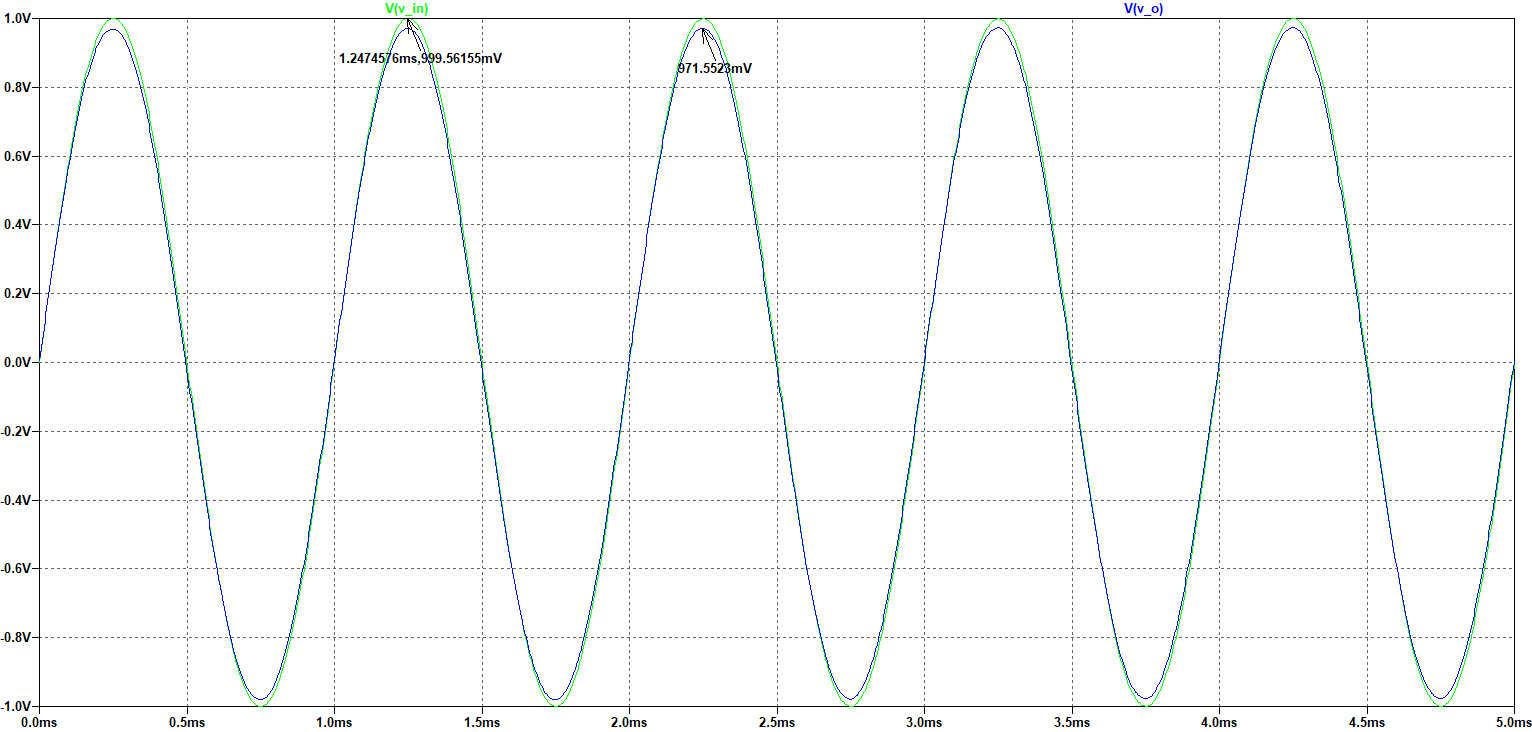
\includegraphics[width=\textwidth]{Imagenes/sim_voep.png}
          \caption{Simulación del voltaje de salida y entrada de la EP en tiempo}
          \label{fig:voep}
        \end{figure}

        Como Se puede apreciar en la imagen, se tiene en la simulación una ganancia de tensión casi 1.

        $$A_v=\dfrac{971.5523 m\volt}{999.5615 m\volt}= 0.971 \approx 1, $$

        siendo este valor el esperado.

        \textbf{Simulación para hallar la impedancia de entrada}

        Como se observa en la figura \ref{fig:zinep}, se tienen los valores pico de cada salida de voltaje de esta manera, haciendo uso de la ecuación \ref{eqn:zin}, tenemos lo siguiente:

        \begin{align*}
          Z_{in} & = V_i \dfrac{R_p}{V_g-V_i}      \\[0.2cm]
          Z_{in} & =\dfrac{646.86m(6k)}{1-646.86m} \\[0.2cm]
          Z_{in} & =10.99k\ohm                     \\[0.2cm]
        \end{align*}

        \begin{figure}[H]
          \centering
          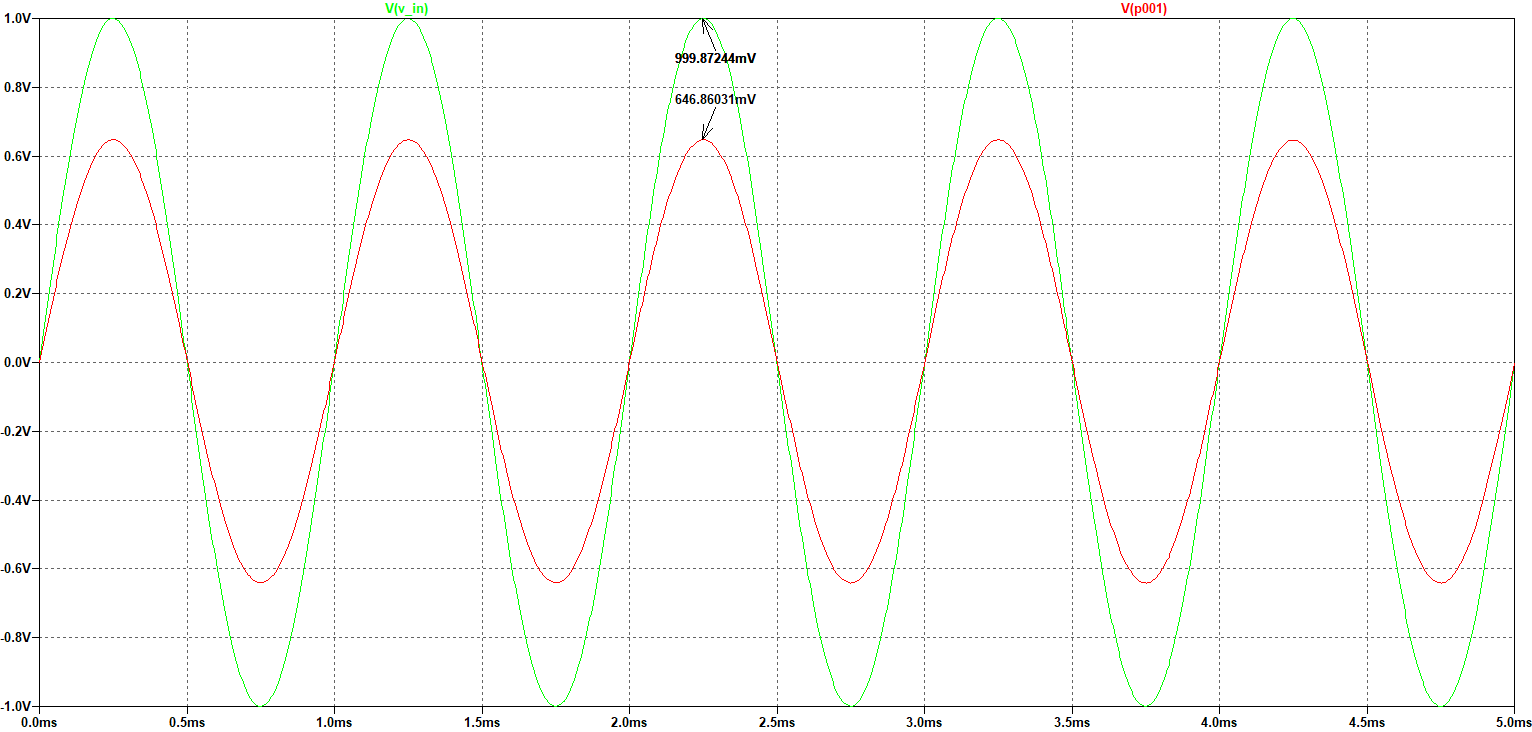
\includegraphics[width=\textwidth]{Imagenes/zinep.png}
          \caption{Simulación del voltaje de salida y entrada de la EP en tiempo para hallar la impedancia de entrada.}
          \label{fig:zinep}
        \end{figure}

        \textbf{Impedancia de salida}

        En este apartado, se va a establecer la impedancia de salida con la ecuación \ref{eqn:zo}, pero bajo las simulaciones realizadas previamente para la metodología adecuada del laboratorio.

        \begin{figure}[H]
          \centering
          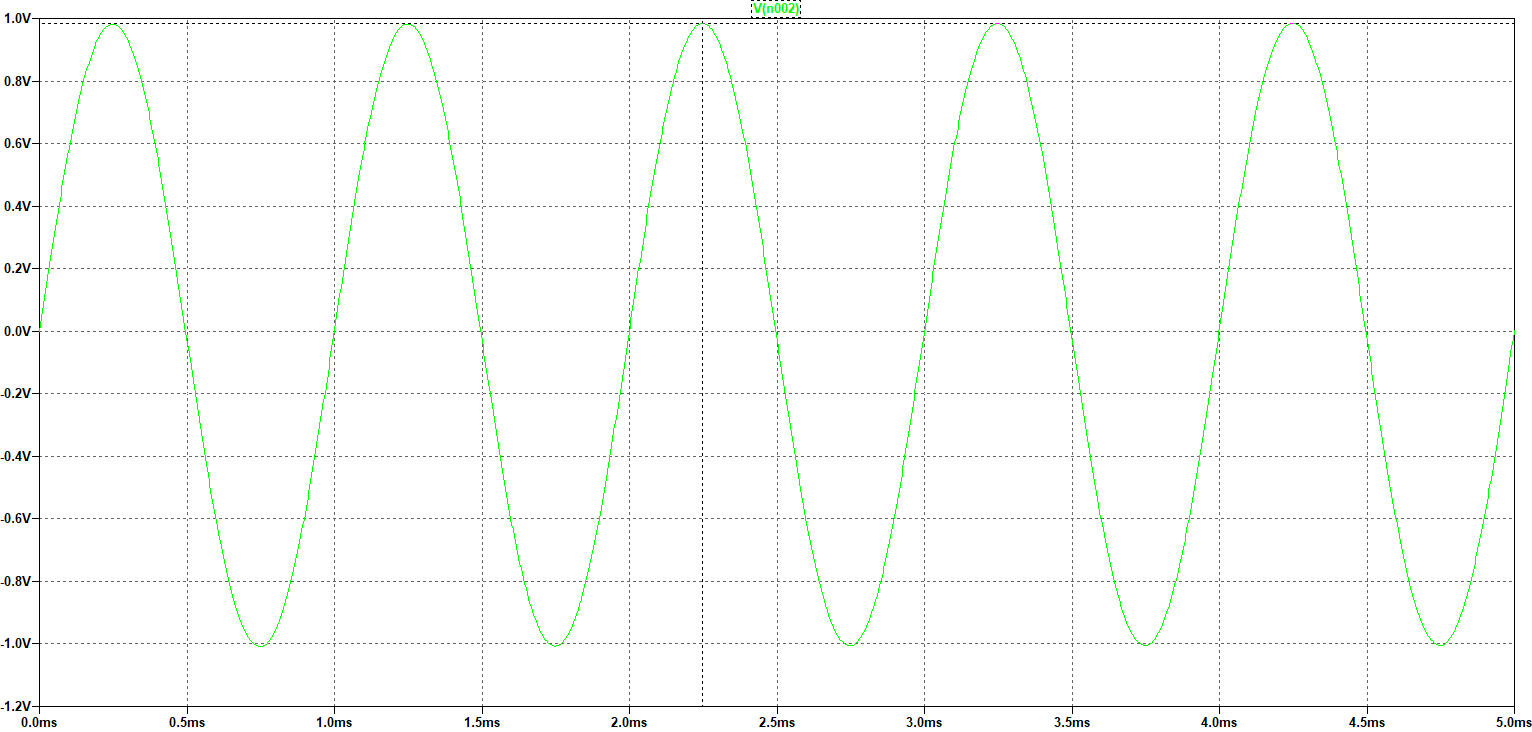
\includegraphics[width=\textwidth]{Imagenes/vo_sc_ep.png}
          \caption{Simulación del voltaje de salida sin carga de la ED en tiempo para hallar la impedancia de salida.}
          \label{fig:vo_sc_ep}
        \end{figure}

        En la figura \ref{fig:vo_sc_ep}, se visualiza el voltaje de salida sin carga, ahora se usara el valor de la simulación de la figura \ref{fig:vo_cc_ep}, y hallar la impedancia de salida.

        \begin{figure}[H]
          \centering
          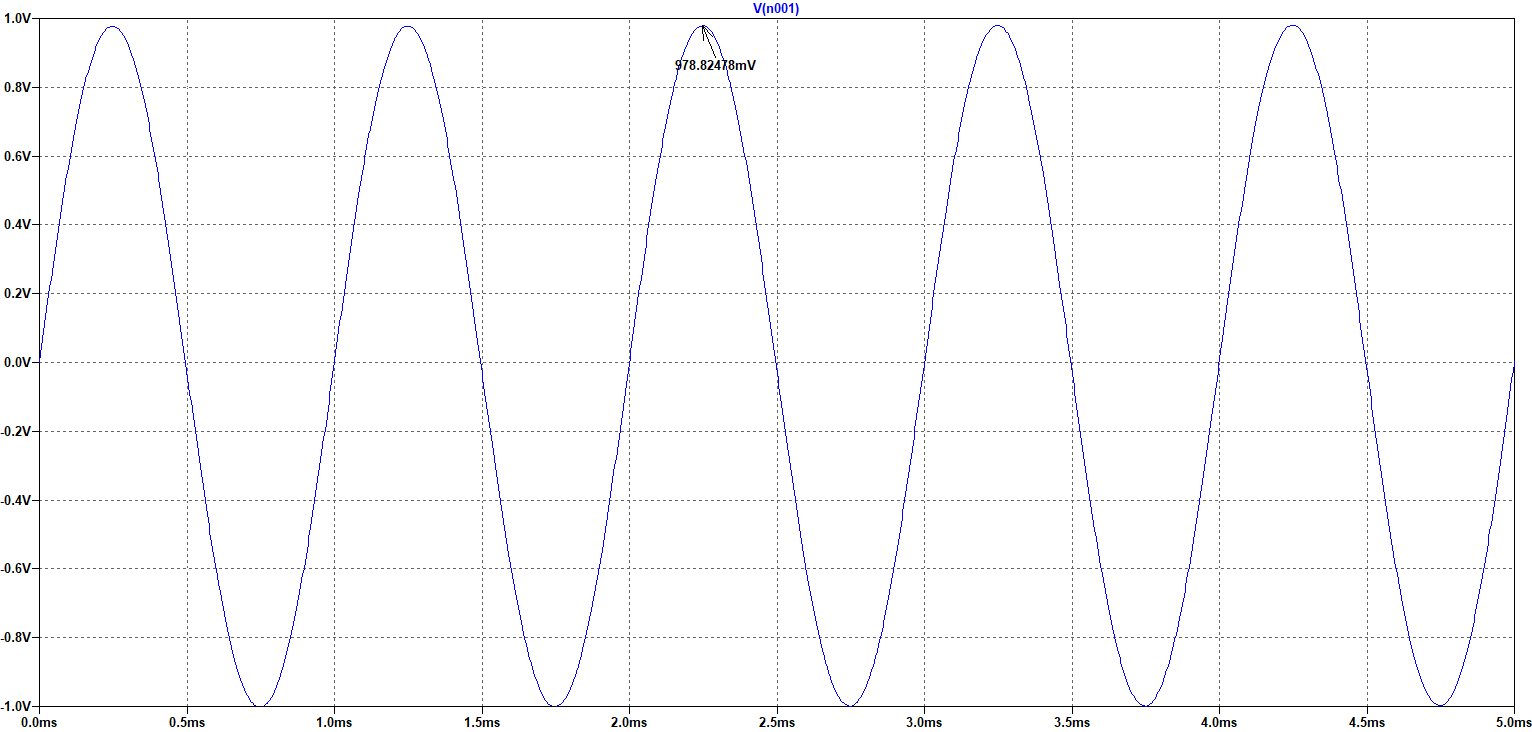
\includegraphics[width=\textwidth]{Imagenes/vo_cc_ep.png}
          \caption{Simulación del voltaje de salida con carga de la EP  en tiempo para hallar la impedancia de salida.}
          \label{fig:vo_cc_ep}
        \end{figure}

        \begin{align*}
          Z_{out} & = \dfrac{V_{osc}R_p - V_{occ}R_p}{V_{occ}} \\[0.2cm]
          Z_{out} & =\dfrac{(1.982-1.593)80}{1.593}            \\[0.2cm]
          Z_{out} & =19.535 \, \ohm                            \\[0.2cm]
        \end{align*}

        \begin{table}[H]
          \centering
          \begin{tabular}{|c|c|c|}
            \hline
            $\mathbf{A_v}$ & $\mathbf{Z_{in}[\ohm]}$ & $\mathbf{Z_{out} [\ohm]}$ \\ \hline
            0.971          & 10.99k                  & 19.535                    \\ \hline
          \end{tabular}
          \caption{Ganancia e impedancias simuladas de la Etapa de potencia}
          \label{tab:dinamico_ep_sim}
        \end{table}


\end{enumerate}

\subsection{Parte 2. Amplificador diferencial}

\begin{enumerate}
  \item \textbf{Identifique la etapa diferencial (ED) en el amplificador base (figura \ref{fig:amplificador_base}).}

        \begin{figure}[H]
          \centering
          \adjustbox{width = 5cm}{\begin{circuitikz}\draw
     \differential{dif}{out 3}
     (0,0) to [short,-o, label=$V_{o}$] ++(1,0) 
    (dif-in 1)  to[C,l=$C_{1}$,*-*] ++(-2,0) to[short,-o, label=$V_{in}$] ++(-0.5,0) (power-in 2) ++(0,10.75) node[vcc](VCC){$10\volt$} ++(0,-12.25) node[vee](VEE){$-10\volt$}
;\end{circuitikz}}
          \caption{Diagrama Esquemático de la etapa  diferencial}
          \label{fig:amplificador_diferencial}
        \end{figure}

        La etapa diferencial es la que se observa en la figura \ref{fig:amplificador_diferencial}, que se ve reflejada también en la figura \ref{fig:amplificador_base}, siendo la primera etapa del amplificador base.

  \item \textbf{Determinar los puntos de reposo de todos los transistores en la ED.}

        En esta etapa, los transistores $Q_1$ y $Q_2$ son iguales, debido a esto los puntos de operación de uno es igual para el otro.

        Hay que tener en cuenta que se tomará en cuenta lo dicho anteriormente con los transistores complementarios, debido a no estar bajo la misma oblea, ambos pueden tener pequeñas variaciones apreciables en su ganancia.

        \subsubsection{Análisis DC}

        Entonces, se tiene lo siguiente:

        \begin{align}
          Q_1=Q_2 \label{eqn:qeq} \\[0.2cm]
          I_{CQ_1}=I_{CQ_2}       \\[0.2cm]
          V_{CEQ_1}=V_{CEQ_2}
        \end{align}

        Tomando en cuenta esas consideraciones, la resistencia $R_5$ no sé tomará en cuenta en DC, ya que la caída de tensión entre sus puntos son iguales debido a la ecuación \ref{eqn:qeq}, por consiguiente, se trabajará con una sola configuración de los dos transistores.

        Simplificando el circuito de la polarización universal de la figura \ref{fig:universall}, obtenemos un $V_{th}$ y una $R_{th}$

        \begin{figure}[H]
          \centering
          \adjustbox{width = 3cm}{

\begin{circuitikz}\draw
     \universall{uni}{out 3}
     (0,0) to [short,-o, label=$V_{o}$] ++(1,0) 
    (dif-in 1)  to[C,l=$C_{1}$,*-*] ++(-2,0) to[short,-o, label=$V_{in}$] ++(-0.5,0) (power-in 2) ++(0,10.75) node[vcc](VCC){$10\volt$} ++(0,-12.25) node[vee](VEE){$-10\volt$}
;\end{circuitikz}}
          \caption{Polarización universal para el estudio del amplificador diferencial}
          \label{fig:universall}
        \end{figure}

        Se aplica divisor de tensión y superposición para hallar el  $V_{th}$:

        \begin{align*}
          V_{th} & = \dfrac{V_{CC}R_{2}}{R_1+R_2}+\dfrac{V_{EE}R_{1}}{R_1+R_2} \\[0.2cm]
          V_{th} & = \dfrac{10(100k)}{100k+100k}+\dfrac{-10(100k)}{100k+100k}  \\[0.2cm]
          V_{th} & = 5-5 = 0\volt                                              \\[0.2cm]
        \end{align*}

        Seguidamente se halla $R_{th}$
        \begin{align*}
          R_{th}=R_1||R_2=100k||100k=50k\ohm
        \end{align*}



        Aplicando la ecuación \ref{eqn:ic} y \ref{eqn:ie_ib}, se obtiene lo siguiente:
        $I_B$ se halla en un recorrido de lazo cerrado, de la base al emisor con el circuito simplificado
        \begin{align*}
          I_{CQ_1} & =\beta \dfrac{10-V_{BE_1}}{R_{th}+R_4(1+\beta)} \\[0.2cm]
          I_{CQ_1} & =\beta \dfrac{10-0.65}{50k+15k(151)}            \\[0.2cm]
          I_{CQ_1} & =605.832 \mu A                                  \\[0.2cm]
        \end{align*}

        Finalmente aplicando LVK por $V_{CE}$, se tiene


        \begin{align*}
          0         & =10-I_{CQ_1}(4.7k)-V_{CEQ_1}-\left(\dfrac{1+\beta}{\beta}\right)I_C(15k)+10 \\[0.2cm]
          V_{CEQ_1} & =20-I_{CQ_1}((4.7k)+\left(\dfrac{1+\beta}{\beta}\right)(15k))               \\[0.2cm]
          V_{CEQ_1} & = 8\volt                                                                    \\[0.2cm]
        \end{align*}

        \begin{table}[H]
          \centering
          \begin{tabular}{|c |c |c|}
            \hline %Lïnea horizontal
            \textbf{Transistor} & $\mathbf{I_{CQ}[\mu A]}$ & $\mathbf{V_{CEQ}[\volt]}$ \\
            \hline
            1                   & 605.832                  & 8                         \\
            \hline
            2                   & 605.832                  & 8                         \\
            \hline
          \end{tabular}
          \caption{Puntos de operación teóricos de la ED}
          \label{tab:ptos_ed}
        \end{table}

        \subsubsection{Análisis en AC}

  \item \textbf{Determine el modelo dinámico del amplificador diferencial a frecuencias medias superponiendo ambos modos. ( Ganancias diferencial y común, impedancias de entrada diferencial y común e impedancia de salida)}

        Como el anterior estudio del análisis en AC, acá se usaran las mismas ecuaciones y por consiguiente, se va a enfocar en colocar las ecuaciones y se darán los resultados de una manera directa para resumir cuentas.

        Se hallará $g_{m_1}$ y $r_{\pi_1}$, recordando que $Q_1=Q_2$, así tenemos que $g_{m_1}=g_{m_2}$ y $r_{\pi_1}=r_{\pi_2}$.

        \begin{align*}
          r_{\pi_1}= \beta \dfrac{V_T}{I_{CQ_5}} & =150 \dfrac{25.851 mA}{605.83 \mu A} \nonumber \\[0.2cm]
          r_{\pi_5}                              & =6.4k \ohm
        \end{align*}

        \begin{align*}
          g_{m_1} & =\dfrac{I_{CQ_5}}{V_T}=\dfrac{605.83 \mu A}{25.851 mA} \nonumber \\[0.2cm]
          g_{m_5} & =23.435m \mho
        \end{align*}


        \textbf{Ganancia de tensión}

        Para hallar la ganancia de tensión de un amplificador diferencial existen dos modos, denominados \textbf{Modo diferencial y Modo Común}, y cada uno de ellos posee una configuración distinta, sin embargo son sencillas de comprender topológicamente.

        En este apartado usaremos las ecuaciones \ref{eqn:ac} y  \ref{eqn:ad}.

        \begin{itemize}
          \item \textbf{Modo diferencial}
                En este punto, la topología a visualizar en modo diferencias es la que se ve en la figura \ref{fig:amplificador_diferencial}, siendo las entradas las bases de los transistores $Q_1$ y $Q_2$, sin embargo, acá solo se tiene una entrada que es por la base de $Q_1$, ya conociendo esto se procede a los cálculos de ganancia de tensión. (Aplica de igual manera para la impedancia en modo diferencial)


                \textbf{Nota:} en modo diferencial tomamos en cuenta la resistencia $R_5$ debido a la configuración que se ve en la figura \ref{fig:amplificador_diferencial}, el recorrido de su corriente es por $R_5$, ya que $R_4$ y $R_7$ son mucho mas grande que $R_5$, además que al no estar en modo común, pasa una corriente distinta por ambas entradas, de esta manera, tiene la posibilidad de solo tomar en cuenta $R_5$ y despreciar la corriente que pasa por $R_4$ y $R_7$. Por el contrario, en modo Común, al tener la misma entrada y ésta dividirse en dos, entra la misma corriente, debido a eso las corrientes que pasa por $R_5$ se anulan, permitiendo que no se desprecie la corriente que pasa por $R_4$ y $R_7$. Por lo tanto, este análisis facilita la obtención de sus ganancias e impedancias de una manera más óptima.
                \begin{align*}
                  A_d & = -\dfrac{(g_{m_1}r_{\pi_1})R_3}{r_{\pi_1}+(g_{m_1}r_{\pi_1}+1)\left(R_{5}+\dfrac{r_{\pi_2}}{(g_{m_2}r_{\pi_2}+1)}\right) } \\[0.2cm]
                  A_d & = -2.95 \approx 3                                                                                                           \\[0.2cm]
                \end{align*}
          \item \textbf{Modo común}
                La topología de esta configuración es haciendo las entradas una sola, es decir hacemos un corto circuito entre las bases de $Q_1$ y $Q_2$, logrando tener un modo común con la entrada de la señal de la fuente, por esa razón su nombre.
                \begin{align*}
                  A_c & =- \dfrac{(g_{m_1}r_{\pi_1})R_3}{r_{\pi_1}+(g_{m_1}r_{\pi_1}+1)R_{4}} \\[0.2cm]
                  A_c & = -0.31                                                               \\[0.2cm]
                \end{align*}
        \end{itemize}
        \newpage
        \textbf{Modelo de Impedancias}

        \begin{itemize}
          \item \textbf{Impedancia en modo diferencial}
                Acá manejamos la misma topología que en ganancia, al igual que su recorrido de corriente.
                \begin{align}
                  Z_d   & = R_{1}||R_{2}||(r_{\pi_1}+ (g_{m_1}r_{\pi_1}+1)
                  \left(R_{5}+\dfrac{r_{\pi_2}}{(g_{m_2}r_{\pi_2}+1)}\right)) \nonumber \\[0.2cm]
                  Z_d   & = R_{1}||R_{2}||(2r_{\pi_1}+
                  R_{5}(g_{m_1}r_{\pi_1}+1))\nonumber                                   \\[0.2cm]
                  Z_{d} & = 41.36k\ohm \label{eqn:zd}
                \end{align}

          \item \textbf{Impedancia en modo común}
                \begin{align*}
                  Z_c & =R_1||R_2||r_{\pi_1}+(g_{m_1}r_{\pi_1}+1)R_{4} \\[0.2cm]
                  Z_c & =48.82k \ohm                                   \\[0.2cm]
                \end{align*}

          \item \textbf{Impedancia de Salida}
                \begin{align*}
                  Z_{out} & =R_3       \\[0.2cm]
                  Z_{out} & =4.7k \ohm \\[0.2cm]
                \end{align*}


          \item \textbf{Nota:} Una acotación importante es que en este apartado se da lo que conocemos como \textbf{CMRR}, como se observa en la ecuación \ref{eqn:cmrr}, si se analiza, se tiene que si $\mathbf{A_d}$ aumenta se va a obtener una mayor ganancia evitando el $\mathbf{CMRR}$ siendo este valido cuando $\mathbf{CMRR=\rho \geq 100db}$, para que esto ocurra de una mejor manera $\mathbf{A_c}$ debería dar muy bajo, para poder su efecto de rechazo alto.

                Para eso realizamos este calculo, para poder ver si existe una buena ganancia. Sin embargo, de no tener una diferencia de potencial en las dos entradas AC no existirá una ganancia.
        \end{itemize}

        \begin{table}[H]
          \centering
          \begin{tabular}{|c|c|c|c|c|c|}
            \hline
            $\mathbf{A_v}$ & $\mathbf{A_C}$ & $\mathbf{Z_{d}[\ohm]}$ & $\mathbf{Z_{c}[\ohm]}$ & $\mathbf{Z_{out} [\ohm]}$ & $\mathbf{\rho [dB]}$ \\ \hline
            -2.95          & -0.31          & 41.36 k                & 48.85k                 & 4.7k                      & 19.57                \\ \hline
          \end{tabular}
          \caption{Ganancia e impedancias teóricas de la Etapa diferencial}
          \label{tab:dinamico_ed}
        \end{table}

        \subsubsection{Simulación}

  \item Realice la simulación de la etapa con el fin de verificar los cálculos de los puntos de operación y el
        modelo dinámico.

        \begin{table}[H]
          \centering
          \begin{tabular}{|c|c|c|}
            \hline
            \textbf{Tag} & \textbf{Puntos de operación} & \textbf{Unidad} \\
            \hline
            V(v\_ce2)    & 8.850259                     & voltage         \\\hline
            V(v\_ce1)    & 7.207804                     & voltage         \\\hline
            Ic(Q1)       & 7.57E-04                     & device\_current \\\hline
            Ic(Q2)       & 4.53E-04                     & device\_current \\
            \hline
          \end{tabular}
          \caption{Simulación de los puntos de operación de la ED}
          \label{tab:ptos_ope_ed}
        \end{table}

        Se aprecian unas diferencias, se calcularan los errores relativos porcentuales, estas diferencias se deben a que son el mismo encapsulado y poseen las mismas características y especificaciones, pero ambos están creado bajos distintas obleas de silicio.

        \begin{itemize}
          \item $\mathbf{V_{CE_1}}$
                \begin{align*}
                  V_{CE_1}=7.21\volt
                  E_r & =\dfrac{|8-7.21|}{8}\cdot 100 \\[0.2cm]
                  E_r & =9.875\%
                \end{align*}

          \item $\mathbf{V_{CE_2}}$
                \begin{align*}
                  V_{CE_2}=8.85\volt
                  E_r & =\dfrac{|8-8.85|}{8}\cdot 100 \\[0.2cm]
                  E_r & =3.125\%
                \end{align*}

          \item $\mathbf{I_{CQ_1}}$
                \begin{align*}
                  I_{CQ_1} & =757 \mu A                                    \\[0.2cm]
                  E_r      & =\dfrac{|605.832\mu-757\mu|}{425\mu}\cdot 100 \\[0.2cm]
                  E_r      & =24.34\%
                \end{align*}
          \item $\mathbf{I_{CQ_2}}$
                \begin{align*}
                  I_{CQ_2} & =453 \mu A                                    \\[0.2cm]
                  E_r      & =\dfrac{|605.832\mu-453\mu|}{425\mu}\cdot 100 \\[0.2cm]
                  E_r      & =25.23\%
                \end{align*}
        \end{itemize}


        Como se puede apreciar, cada uno de los errores relativos porcentuales no son despreciables, pero validos para los cálculos teóricos realizados, se aproximan bastante a los posibles. Más adelante sabremos si nos acercamos bastante a los valores experimentales o reales.
        \newpage
        \textbf{Simulación de ganancia en tiempo}

        \begin{figure}[H]
          \centering
          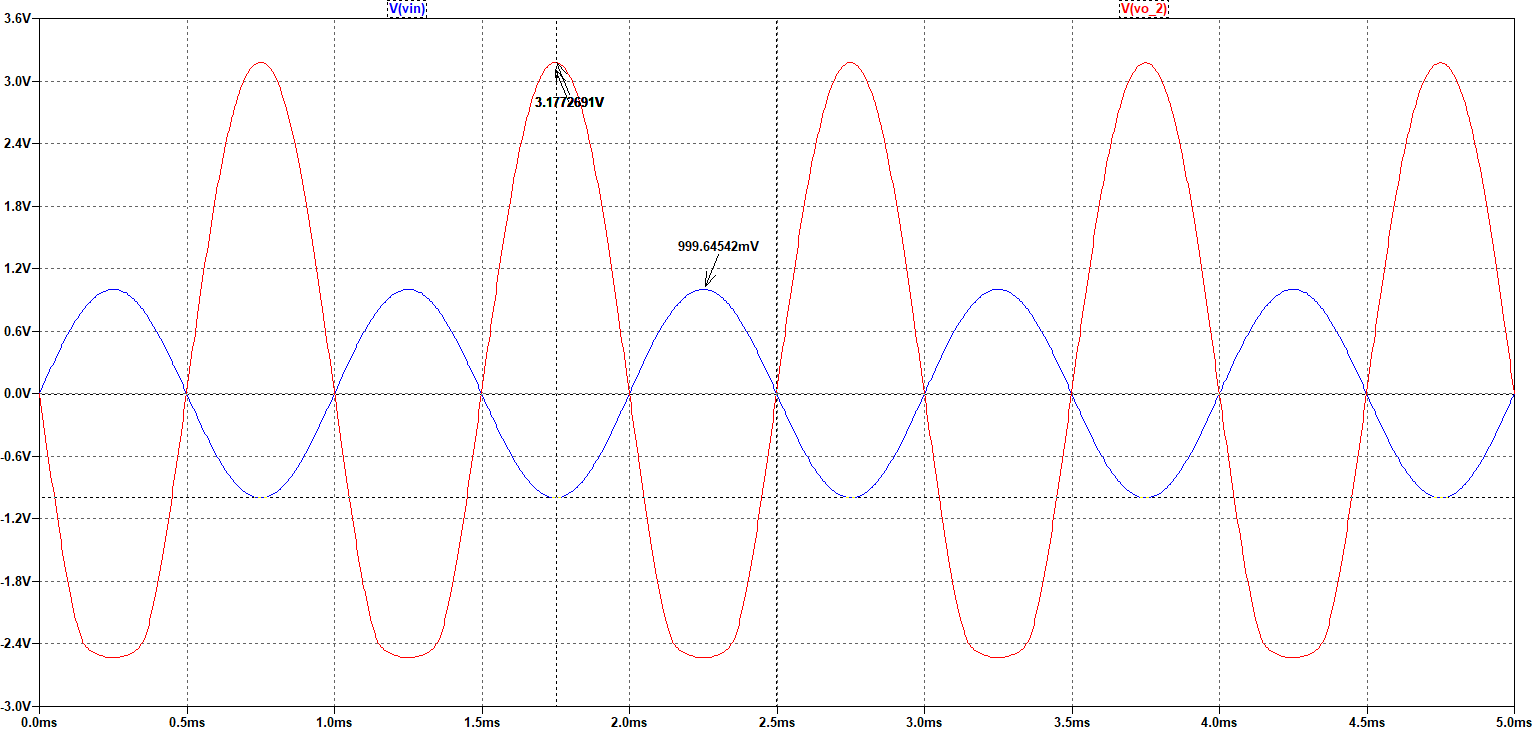
\includegraphics[width=\textwidth]{Imagenes/sim_voed.png}
          \caption{Simulación del voltaje de salida y entrada de la ED en tiempo}
          \label{fig:voed}
        \end{figure}

        Como Se puede apreciar en la imagen, se tiene en la simulación una ganancia de tensión de:

        $$A_v=\dfrac{3.1772691\volt}{0.99964542\volt}= 3.178, $$

        siendo este valor el esperado.

        \begin{itemize}
          \item \textbf{Nota: } Se calculo la ganancia e indico un valor negativo, esto es debido al desfase que ocurre que es de 180°, y que posee una ganancia donde entra por base y sale por colector, podría verse como una configuración de emisor-Común estando dos en paralelo.

                Por consiguiente, la figura \ref{fig:voed} se pueden apreciar el desfase y su ganancia. Comportándose en la zona lineal por la polarización universal.
        \end{itemize}

        \textbf{Simulación para hallar la impedancia en modo diferencial}

        Como se observa en la figura \ref{fig:zded}, se tienen los valores pico de cada salida de voltaje de esta manera, haciendo uso de la ecuación \ref{eqn:zin}, tenemos lo siguiente:

        \begin{align*}
          Z_{d} & = V_i \dfrac{R_p}{V_g-V_i}           \\[0.2cm]
          Z_{d} & =\dfrac{520.066m(41.5k)}{1-520.066m} \\[0.2cm]
          Z_{d} & =\dfrac{520.066m(41.5k)}{1-520.066m} \\[0.2cm]
          Z_{d} & =44.97k\ohm                          \\[0.2cm]
        \end{align*}

        \begin{figure}[H]
          \centering
          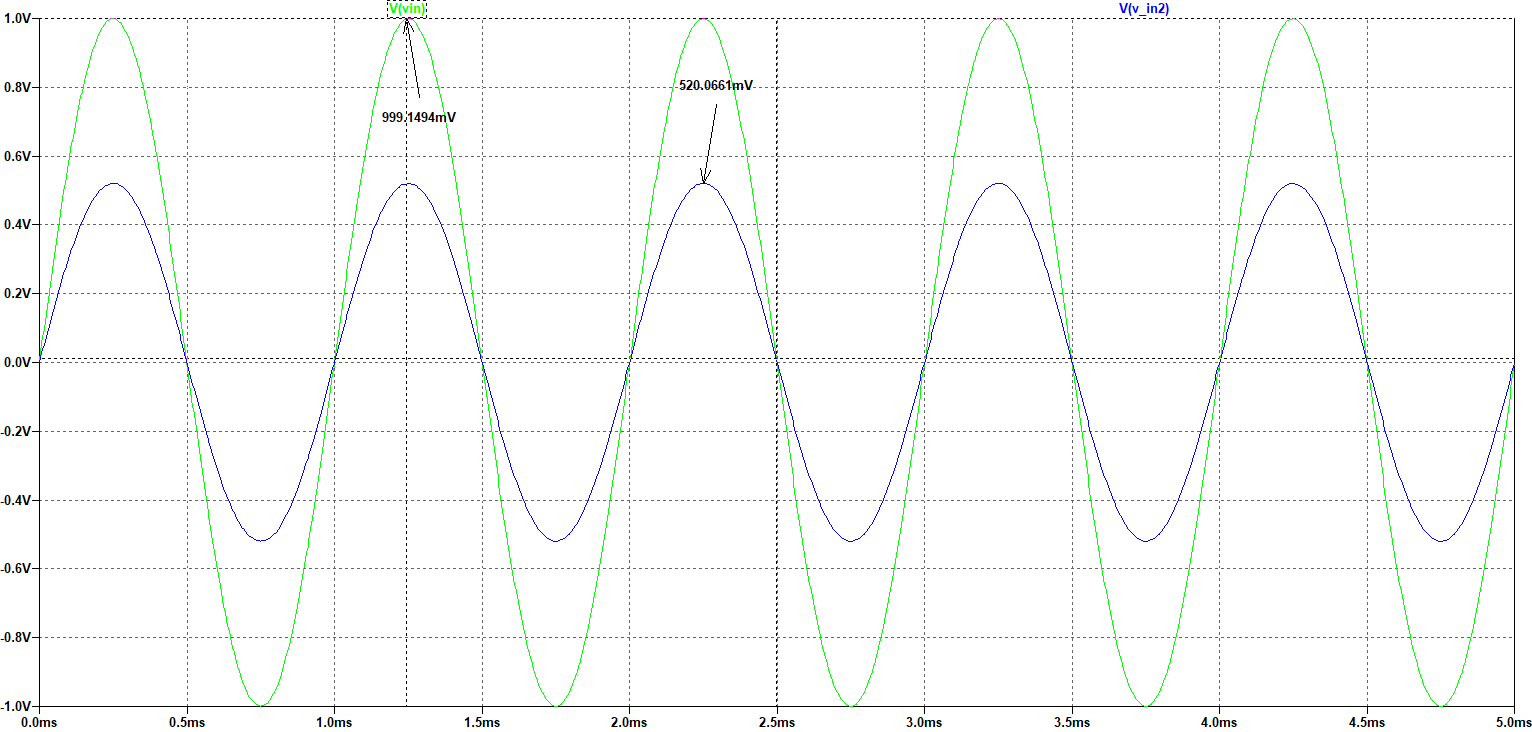
\includegraphics[width=\textwidth]{Imagenes/zd_ed.png}
          \caption{Simulación del voltaje de salida y entrada de la ED en tiempo para hallar la impedancia en modo diferencial.}
          \label{fig:zded}
        \end{figure}

        \textbf{Simulación para hallar la impedancia en modo común}

        Como se observa en la figura \ref{fig:zced}, se tienen los valores pico de cada salida de voltaje de esta manera, haciendo uso de la ecuación \ref{eqn:zc}, tenemos lo siguiente:

        \begin{align*}
          Z_{c}            & = 2V_i \dfrac{R_p}{V_g-V_i}         \\[0.2cm]
          Z_{c}            & =2\dfrac{520.066m(50k)}{1-520.066m} \\[0.2cm]
          Z_{c}            & =2\dfrac{520.066m(50k)}{1-520.066m} \\[0.2cm]
          Z_{c}            & =108.36k\ohm                        \\[0.2cm]
          \dfrac{Z_{c}}{2} & =54.18k\ohm                         \\[0.2cm]
        \end{align*}

        \begin{figure}[H]
          \centering
          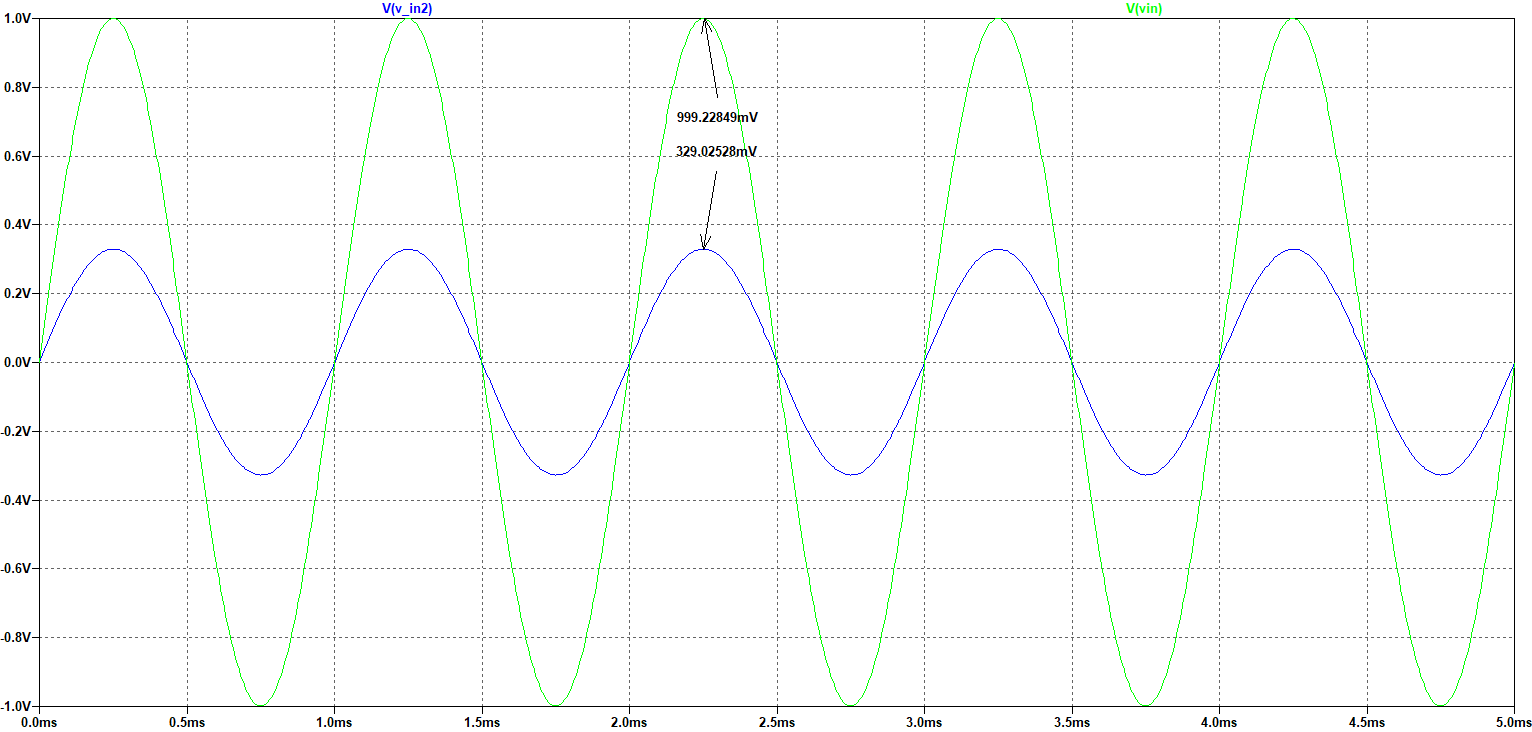
\includegraphics[width=\textwidth]{Imagenes/zc_ed.png}
          \caption{Simulación del voltaje de salida y entrada de la ED en tiempo para hallar la impedancia en modo común.}
          \label{fig:zced}
        \end{figure}

        \textbf{Impedancia de salida}

        En este apartado, se va a establecer la impedancia de salida con la ecuación \ref{eqn:zo}, pero bajo las simulaciones realizadas previamente para la metodología adecuada del laboratorio.

        \begin{figure}[H]
          \centering
          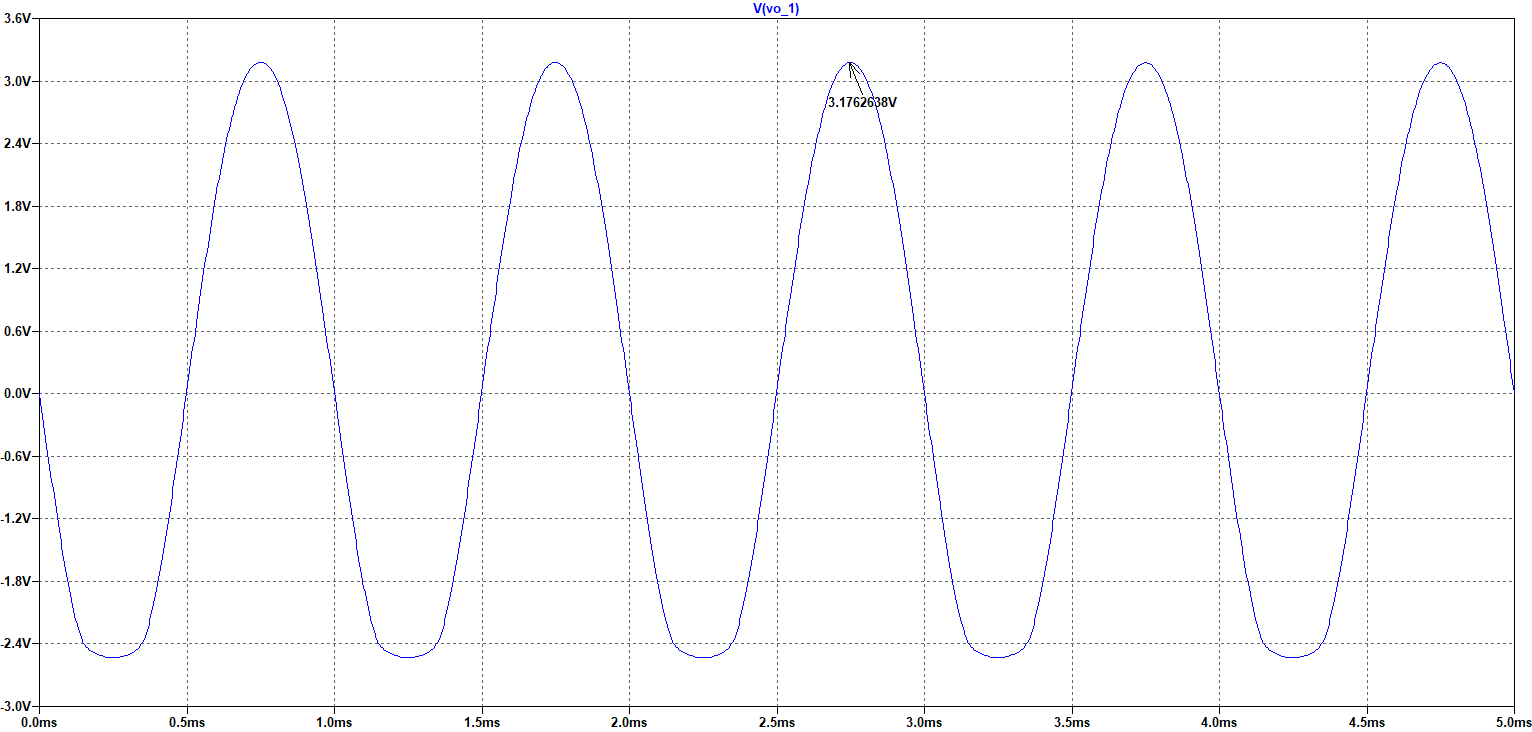
\includegraphics[width=\textwidth]{Imagenes/vosc.png}
          \caption{Simulación del voltaje de salida sin carga de la ED en tiempo para hallar la impedancia de salida.}
          \label{fig:vo_sc_ed}
        \end{figure}

        En la figura \ref{fig:vo_sc_ed}, se visualiza el voltaje de salida sin carga, ahora se usara el valor de la simulación de la figura \ref{fig:vo_cc_ed}, y hallar la impedancia de salida.

        \begin{figure}[H]
          \centering
          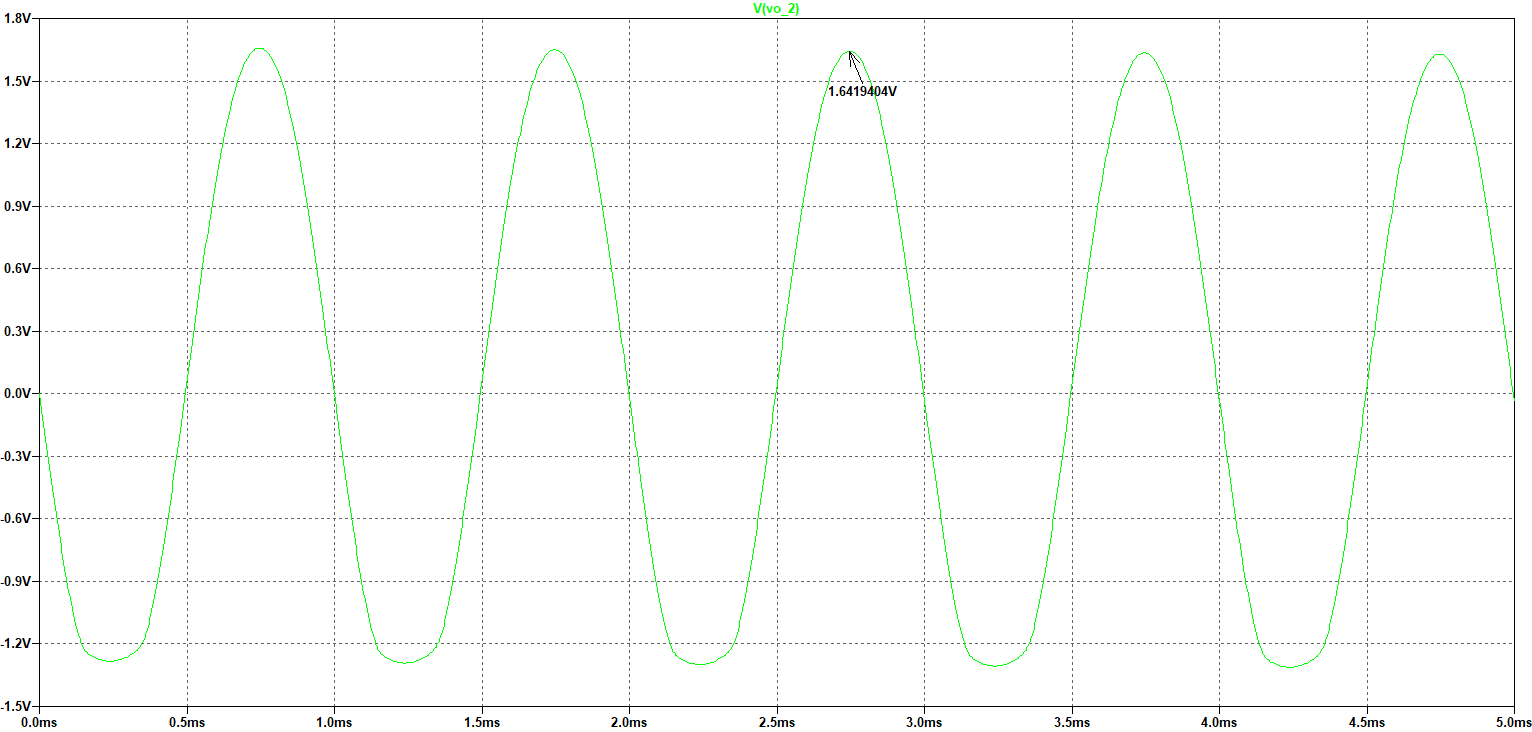
\includegraphics[width=\textwidth]{Imagenes/vocc.png}
          \caption{Simulación del voltaje de salida con carga de la ED en tiempo para hallar la impedancia de salida.}
          \label{fig:vo_cc_ed}
        \end{figure}

        \begin{align*}
          Z_o     & = \dfrac{V_{osc}R_p - V_{occ}R_p}{V_{occ}} \\[0.2cm]
          Z_{out} & =\dfrac{(3.17626-1.64194)5k}{1.64194}      \\[0.2cm]
          Z_{out} & =4.67k                                     \\[0.2cm]
        \end{align*}

        \begin{table}[H]
          \centering
          \begin{tabular}{|c|c|c|c|}
            \hline
            $\mathbf{A_v}$ & $\mathbf{Z_{d}[\ohm]}$ & $\mathbf{Z_{c}[\ohm]}$ & $\mathbf{Z_{out} [\ohm]}$ \\ \hline
            -3.178         & 44.97k                 & 54.18k                 & 4.67k                     \\ \hline
          \end{tabular}
          \caption{Ganancia e impedancias simuladas de la Etapa diferencial}
          \label{tab:dinamico_ed_sim}
        \end{table}

\end{enumerate}

\subsection{Parte 3. Amplificador multietapas}

\begin{enumerate}
  \item \textbf{Para cada etapa por separado del amplificador base (figura \ref{fig:amplificador_base}) determine: Punto de operación de los elementos activos y modelo dinámico de las etapas amplificadoras. Utilice como carga $R_L$ la indicada en el anexo ($R_L=2.2k\ohm$).}

        Los puntos operacionales de la etapa de potencia están reflejados en la tabla \ref{tab:ptos_ep} y los de la etapa diferencial en la tabla \ref{tab:ptos_ed}.

        Los puntos del modelo dinámico de la etapa de potencia se hallan en la tabla \ref{tab:dinamico_ep} y la etapa diferencial en la tabla \ref{tab:dinamico_ed}.

        \subsubsection{Análisis DC}
        Se va a calcular los puntos de operación y modelo dinámico de la etapa impulsora o driver. Se identifica a la etapa impulsora en el amplificador base directamente en la figura \ref{fig:driver}

        \begin{figure}[H]
          \centering
          \adjustbox{width = 3cm}{\begin{circuitikz}\draw
    (0,0)\driver{driv}{out 3} to[C,l=$C_{7}$,*-*]++(3,0) 
;\end{circuitikz}}
          \caption{Diagrama esquemática de la etapa impulsora}
          \label{fig:driver}
        \end{figure}

        En la figura \ref{fig:driver} se tiene el capacitor $C_7$ como capacitor de desacople, $C_6$ es un capacitor denominado de \textbf{bypass}, este nos permite que cuando este en su punto de operación permite una mayor ganancia debido a que tenemos la resistencia $R_{11}$  que ayuda a su punto de operación, pero en AC, no se toma en cuenta gracias al condensador. Por otro lado, permite que al ver la impedancia de $Z_{CCQ_3}$, solo observará $r_0$, a consecuencia de el capacitor de bypass, por el corto generado a frecuencias medias y en AC.

        El condensador $C_4$ se comporta como un abierto al igual que todos las demás capacitores, a diferencia es que los demás se cortocircuitan en frecuencias medias (en AC), este solo se cortocircuita en frecuencias altas, esto se identifica por su valor de capacitancia y que se encuentra entre Base y Colector, manejando el modelo expandido de pi, tomando en cuentas las perdidas en alta frecuencia.

        Al igual que con la etapa de diferencial, se aplica divisor de tensión y superposición para hallar el $V_{th}$.

        Esto es debido a que se simplifica el circuito realizando un circuito equivalente visto desde la base hacia la entrada.

        \begin{align*}
          V_{th} & = \dfrac{V_{CC}R_{10}}{R_{10}+R_{15}}+\dfrac{V_{EE}R_{15}}{R_{10}+R_{15}} \\[0.2cm]
          V_{th} & = \dfrac{10(220k)}{220k+33k}+\dfrac{-10(33k)}{220k+33k}                   \\[0.2cm]
          V_{th} & = 7.4 \volt                                                               \\[0.2cm]
        \end{align*}

        Seguidamente se halla $R_{th}$
        \begin{align*}
          R_{th}=R_{15}||R_{10}=33k||220k=28.7k\ohm
        \end{align*}

        Aplicando LVK, al circuito equivalente de thevenin de la figura \ref{fig:driver}, se halla $I_{CQ_3}$, haremos uso de la ecuación \ref{eqn:ib}

        \begin{align*}
          0        & =10-I_CR_{11}-V_{EB}-I_{B}R_{th}-V_{th}                 \\[0.2cm]
          I_{CQ_3} & =\dfrac{10-V_{BE}-V_{th}}{R_{11}+\dfrac{R_{th}}{\beta}} \\[0.2cm]
          I_{CQ_3} & =\dfrac{10-0.65-7.4}{680+\dfrac{28.7k}{150}}            \\[0.2cm]
          I_{CQ_3} & =2.24mA                                                 \\[0.2cm]
        \end{align*}

        Finalmente, se halla $V_{CEQ_3}$, aplicando LVK por el transistor $Q_3$

        \begin{align*}
          0         & =10-I_{E}(R_{11})-V_{CEQ_3}-I_C(R_{16})+10 \\[0.2cm]
          V_{CEQ_3} & =20-I_{E}(R_{11})-I_C(R_{16})              \\[0.2cm]
          V_{CEQ_3} & = 3.2346\volt                              \\[0.2cm]
        \end{align*}

        \begin{table}[H]
          \centering
          \begin{tabular}{|c |c |c|}
            \hline %Lïnea horizontal
            \textbf{Transistor} & $\mathbf{I_{CQ}[ A]}$ & $\mathbf{V_{CEQ}[\volt]}$ \\
            \hline
            3                   & 2.24m                 & 3.2346                    \\
            \hline
          \end{tabular}
          \caption{Puntos de operación teóricos de la etapa impulsora}
          \label{tab:ptos_ei}
        \end{table}

        \subsubsection{Análisis en AC}
        Se hallará $g_{m_3}$, $r_{\pi_3}$ y $r_0$, recordar que se hace uso de las ecuaciones \ref{eqn:gm}, \ref{eqn:rpi} y \ref{eqn:ro}.

        \begin{align*}
          r_{\pi_3}= \beta \dfrac{V_T}{I_{CQ_3}} & =150 \dfrac{25.851 mA}{2.24 mA} \nonumber \\[0.2cm]
          r_{\pi_3}                              & =1.732k \ohm
        \end{align*}

        \begin{align*}
          g_{m_3} & =\dfrac{I_{CQ_3}}{V_T}=\dfrac{2.24m A}{25.851 mA} \nonumber \\[0.2cm]
          g_{m_3} & =86.65m \mho
        \end{align*}

        En este caso, $r_0$ es distinto de infinito, debido a que este transistor $Q_3$, posee un capacitor que se tomará en cuenta en altas frecuencias, aplicando el teorema de Miller, por el modelo expandido de pi. Siendo un capacitor asociado a la juntura del transistor.

        \begin{gather}
          r_0=\dfrac{V_A}{I_C}=\dfrac{150}{2.24m} \nonumber \\[0.2cm]
          r_0=67.024 \, K\ohm
        \end{gather}

        \textbf{Ganancia de tensión}

        \begin{align*}
          A_v & =- \dfrac{g_{m_3}r_{\pi_3}R_{16}}{r_{\pi_3}} \\[0.2cm]
          A_v & =- \dfrac{150(6.8k)}{1.732k}                 \\[0.2cm]
          A_v & =- -588.91                                   \\[0.2cm]
        \end{align*}

        Lo que se obtiene como resultado, da una mayor relación como su nombre lo indica, \"impulsora\", en efecto se tiene una ganancia bastante grande, que permite impulsar la señal de la etapa anterior, siendo la de la etapa diferencial.

        \textbf{Impedancia de entrada}

        \begin{align*}
          Z_{in} & = R_{15}||R_{10}||r_{\pi_3} \\[0.2cm]
          Z_{in} & = 1.633k\ohm
        \end{align*}

        \textbf{Impedancia de salida}

        \begin{align*}
          Z_{out} & = R_{16}    \\[0.2cm]
          Z_{out} & = 6.8k \ohm
        \end{align*}

        \begin{table}[H]
          \centering
          \begin{tabular}{|c|c|c|}
            \hline
            $\mathbf{A_v}$ & $\mathbf{Z_{in}[\ohm]}$ & $\mathbf{Z_{out} [\ohm]}$ \\\hline
            -588.91        & 1.633k                  & 6.8k                      \\\hline
          \end{tabular}
          \caption{Ganancia e impedancias teóricas de la Etapa impulsora}
          \label{tab:dinamico_ei}
        \end{table}

  \item \textbf{Acoplando todas las etapas del amplificador base, determine: Punto de operación de los elementos activos
          y modelo dinámico del amplificador completo.}

        Debido a los condensadores de acople y desacople ($C_1$, $C_2$, $C_3$, $C_5$, $C_6$ y $C_7$ ), los puntos de operación se mantienen igual para cada una de las etapas, como se indica anteriormente sus valores se hallan en la tabla \ref{tab:ptos_ed}, \ref{tab:ptos_ep} y \ref{tab:ptos_ei}

        Lo que si cambia es el estudio en su modelo dinámico, debido a la ecuación \ref{eqn:capacitores}, donde cada uno de los capacitores de acople y desacople se comportan como un corto, exceptuando el capacitor $C_4$, donde se realizará un estudio mas detallado en los próximos apartados.


        En este análisis como se están acoplando las distintas etapas, para hallar la Ganancia total, se aplicará la ecuación \ref{eqn:avt}.

        Aunque se representara en la \textbf{tabla \ref{tab:gm_rpi} }
        , donde podemos encontrar de manera inmediata cada uno de los valores de $g_{m}$, $r_\pi$ y $r_o$.

        \begin{table}[H]
          \centering
          \begin{tabular}{|c|c|c|c|}
            \hline
            \textbf{Transistores} & $\mathbf{g_m [\si{\mho}]}$ & $\mathbf{r_\pi [\si{\ohm}]}$ & $\mathbf{r_o [\ohm]}$ \\
            \hline
            1                     & 23.435m                    & 6.4k                         & $\infty$              \\\hline
            2                     & 23.435m                    & 6.4k                         & $\infty$              \\\hline
            3                     & 86.65m                     & 1.732k                       & 67.024k               \\\hline
            5                     & 16.44m                     & 9.124k                       & $\infty$              \\\hline
            6                     & 16.44m                     & 9.124k                       & $\infty$              \\
            \hline
          \end{tabular}
          \caption{Valores de $g_{m}$, $r_\pi$ y $r_o$ del amplificador multietapas}
          \label{tab:gm_rpi}
        \end{table}

        Se tiene en cuenta la tabla ahora se busca la ganancia.

        \textbf{Ganancia de tensión de un amplificador multietapas}

        \begin{itemize}
          \item \textbf{Ganancia en modo Diferencial}

                \begin{align*}
                  A_v          & =A_dA_2A_3                                                                                                                                           \\[1cm]
                  A_d          & =-\dfrac{(g_{m_1}r_{\pi_1})(R_{3}||R_{15}||R_{10}||r_{\pi_3})}{r_{\pi_1}+(g_{m_1}r_{\pi_1}+1)\left(R_5+\dfrac{r_{\pi_2}}{g_{m_2}r_{\pi_2}+1}\right)} \\[0.2cm]
                  A_d          & =-0.755                                                                                                                                              \\[1cm]
                  A_2          & =-\dfrac{(g_{m_3}r_{\pi_3})(R_{16}||R_{17}||R_{12}||(r_{\pi_5}+(g_{m_5}r_{\pi_5}+1)(R_{13}+R_L)))}{r_{\pi_3}}                                        \\[0.2cm]
                  A_2          & =-363.128                                                                                                                                            \\[1cm]
                  A_3          & =\dfrac{(g_{m_5}r_{\pi_5}+1)(R_{13}+R_L)}{r_{\pi_5}+(g_{m_5}r_{\pi_5}+1)(R_{13}+R_L)}\left(\dfrac{R_L}{R_{13}+R_L}\right)                            \\[0.2cm]
                  A_3          & =0.969                                                                                                                                               \\[1cm]
                  A_v          & =-0.755(-363.128)0.969                                                                                                                               \\[0.2cm]
                  \mathbf{A_v} & =\mathbf{265.659} = 20log(265.659)=48.487 db                                                                                                         \\[0.2cm]
                \end{align*}

          \item \textbf{Ganancia en modo Común}

                En este caso, la ganancia de $A_2$ y $A_3$ se mantienen iguales y solo cambia la de la etapa diferencial acoplada con las demás etapas.

                \begin{align*}
                  A_{vc}          & =A_cA_2A_3                                                                                        \\[1cm]
                  A_c             & =-\dfrac{(g_{m_1}r_{\pi_1})(R_{3}||R_{15}||R_{10}||r_{\pi_3})}{r_{\pi_1}+(g_{m_1}r_{\pi_1}+1)R_4} \\[0.2cm]
                  A_c             & =-0.0795                                                                                          \\[1cm]
                  A_2             & =-363.128                                                                                         \\[1cm]
                  A_3             & =0.969                                                                                            \\[1cm]
                  A_{vc}          & =-0.0795 (-363.128 )0.969                                                                         \\[0.2cm]
                  \mathbf{A_{vc}} & =\mathbf{27.973}                                                                                  \\[0.2cm]
                \end{align*}

        \end{itemize}
        \textbf{Impedancia de entrada modo diferencial}

        Se puede observar en el circuito de la figura \ref{fig:amplificador_base}, que la impedancia de entrada es el mismo que la impedancia de entrada en modo diferencial de la etapa diferencial. Por lo tanto, haciendo uso del valor de la ecuación \ref{eqn:zd}, se tiene:
        $$Z_{in}=Z_d=41.36k\si{\ohm}$$



        \textbf{Impedancia de entrada modo común}

        Se puede observar en el circuito de la figura \ref{fig:amplificador_base}, que la impedancia de entrada es el mismo que la impedancia de entrada en modo común de la etapa diferencial. Por lo tanto, haciendo uso del valor de la ecuación \ref{eqn:zc}, se tiene y también sale reflejado en la tabla \ref{tab:dinamico_ed}:
        $$Z_{in}=Z_c=48.82k\si{\ohm}$$

        \textbf{Impedancia de salida}

        Recordar que ayuda mucho observar desde donde estas viendo el circuito y de esa manera empezar allí el recorrido de la corriente para dar el resultado adecuado.

        \begin{align*}
          Z_{out} & =\left(\dfrac{R_L}{R_{13}+R_L}\right)[R_{13}+R_L + \dfrac{r_{\pi_5}]||R_{16}||R_{17}||R_{12}}{g_{m_5}r_{\pi_5}+1} \\[0.2cm]
          Z_{out} & = 27.49 \si{\ohm}
        \end{align*}

        \begin{table}[H]
          \centering
          \begin{tabular}{|c|c|c|c|c|}
            \hline
            $\mathbf{A_v}$ & $\mathbf{A_{vc}}$ & $\mathbf{Z_{d}[\ohm]}$ & $\mathbf{Z_{c}[\ohm]}$ & $\mathbf{Z_{out} [\ohm]}$ \\\hline
            265.659        & 27.91             & 41.36k                 & 48.82k                 & 27.49                     \\\hline
          \end{tabular}
          \caption{Ganancia e impedancias teóricas del amplificador base}
          \label{tab:dinamico_base}
        \end{table}

        En la tabla \ref{tab:dinamico_base}, se observa que se mantiene la impedancia alta de entrada de la etapa diferencial y gracias al acople entre la etapa impulsora con la de potencia, se tiene una impedancia de salida un poco mayor, sin embargo, sigue manteniéndose baja la impedancia de salida.

        \subsubsection{Simulación}
  \item \textbf{Realice la simulación del circuito con el fin de verificar los cálculos previos.}

        Importante recalcar que los puntos de operación se mantienen igual, sin embargo, no se mostraron la simulación de la etapa impulsora, que se muestra a continuación en la tabla \ref{tab:ptos_ope_ei}:

        \begin{table}[H]
          \centering
          \begin{tabular}{|c|c|c|}
            \hline
            \textbf{Tag} & \textbf{Puntos de operación} & \textbf{Unidad} \\
            \hline
            V(v\_ce3)    & -2.48272                     & voltage         \\\hline
            Ic(Q3)       & -0.00234083                  & device\_current \\\hline
          \end{tabular}
          \caption{Simulación de los puntos de operación de la etapa impulsora}
          \label{tab:ptos_ope_ei}
        \end{table}
        \begin{itemize}



          \item \textbf{Ganancia de tensión modo Diferencial}
                \begin{figure}[H]
                  \centering
                  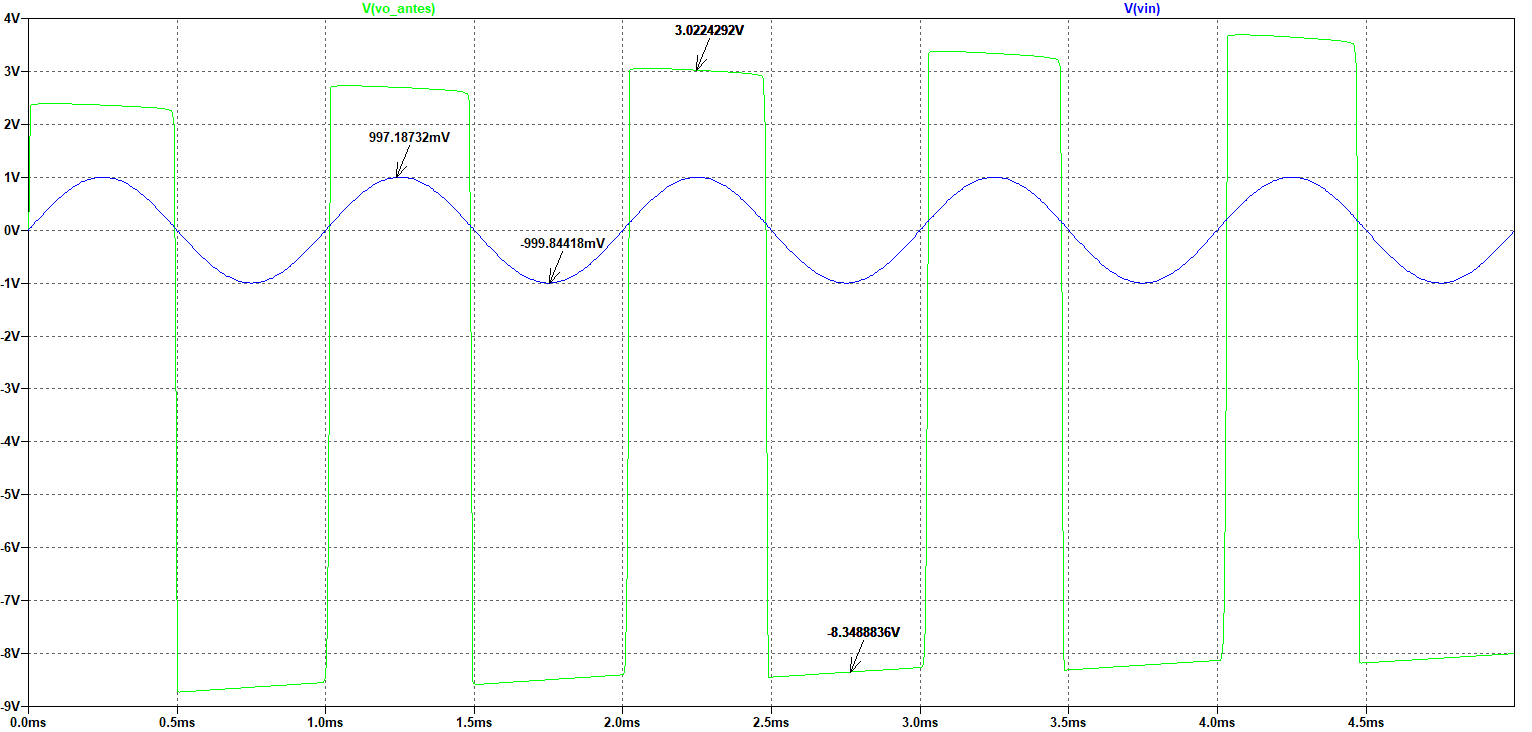
\includegraphics[width=\textwidth]{Imagenes/sim_base_1.png}
                  \caption{Simulación del voltaje de salida y entrada del amplificador base en tiempo con un $V_{in}=1V_p$ en modo diferencial.}
                  \label{fig:sim_base_1}
                \end{figure}

                Se puede observar en la figura \ref{fig:sim_base_1}, que si hallamos la ganancia daría lo siguiente:

                \begin{align*}
                  A_v & =\dfrac{3.022429-(-8.348883)}{997.18732m-(-999.84418m)} \\[0.2cm]
                  A_v & =5.7                                                    \\[0.2cm]
                \end{align*}

                Sin embargo como tiene una ganancia de 378.84, tenemos la salida saturada, como se puede observar, en ese caso usamos un voltaje de entrada de $1m\volt$, como se observa en la figura \ref{fig:sim_base_1m}.

                \begin{figure}[H]
                  \centering
                  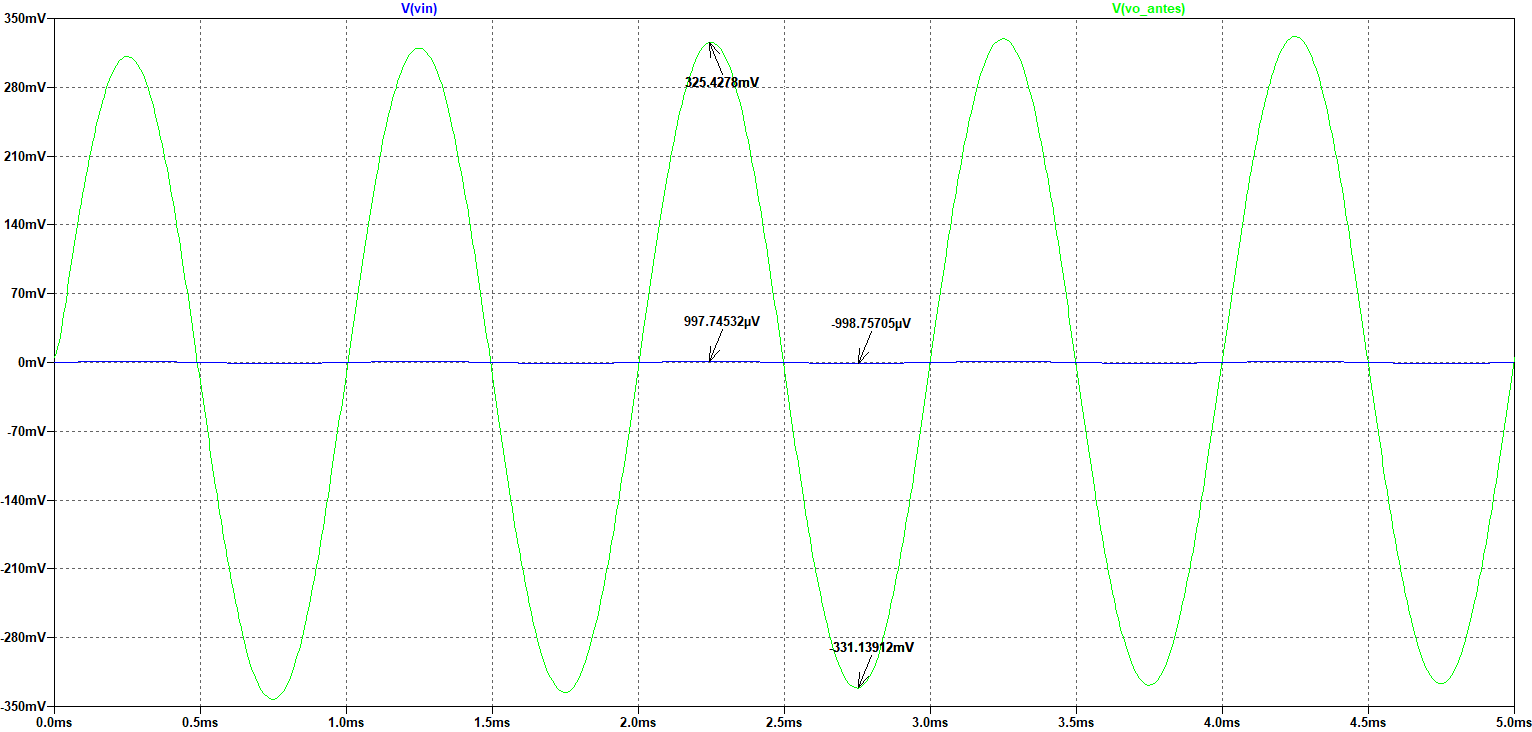
\includegraphics[width=\textwidth]{Imagenes/sim_base_1m.png}
                  \caption{Simulación del voltaje de salida y entrada del amplificador base en tiempo con un $V_{in}=1mV_p$ en modo diferencial.}
                  \label{fig:sim_base_1m}
                \end{figure}

                Acá si podemos ver que no existe una saturación y debido a esto si se ve su verdadera ganancia que seria la siguiente:

                \begin{align*}
                  A_v & =\dfrac{325.4278m-(-331.13912)}{997.74532\mu-(-998.75705\mu)} \\[0.2cm]
                  A_v & =328.86                                                       \\[0.2cm]
                \end{align*}

                Nos da una ganancia aproximada a la calculada, por hallarse en la zona activa, verificando de esa manera que hemos hecho unos cálculos teóricos adecuados.
                \newpage
          \item \textbf{Ganancia de tensión modo Común}

                \begin{figure}[H]
                  \centering
                  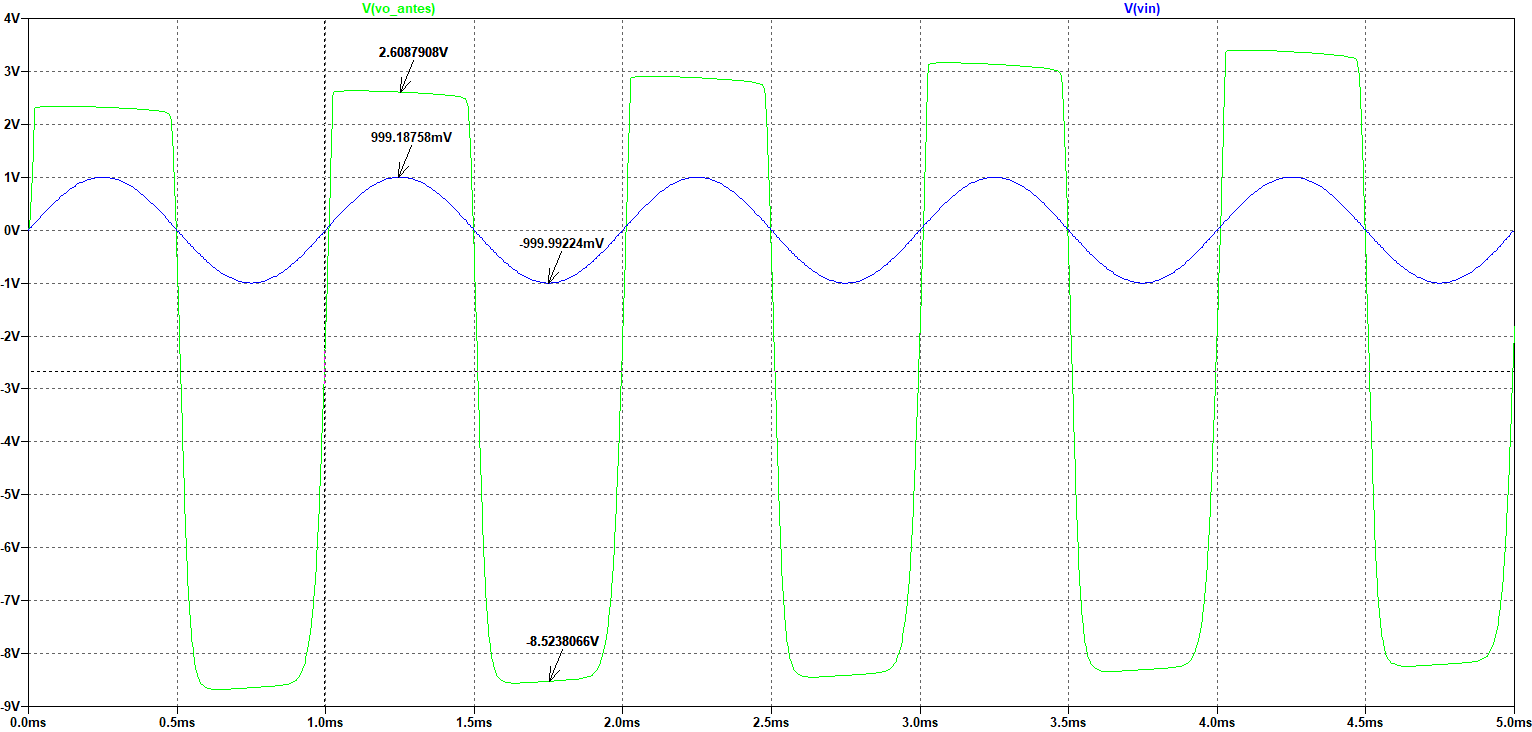
\includegraphics[width=\textwidth]{Imagenes/sim_basecomun_1.png}
                  \caption{Simulación del voltaje de salida y entrada del amplificador base en tiempo con un $V_{in}=1V_p$ en modo común.}
                  \label{fig:sim_basecomun_1}
                \end{figure}

                Se puede observar en la figura \ref{fig:sim_basecomun_1}, que si hallamos la ganancia daría lo siguiente:

                \begin{align*}
                  A_c & =\dfrac{2.6087908-(-8.5238066)}{999.18758m-(-999.99224m)} \\[0.2cm]
                  A_c & =5.6                                                      \\[0.2cm]
                \end{align*}

                Sin embargo como tiene una ganancia de 27.91, tenemos la salida saturada, como se puede observar, en ese caso usamos un voltaje de entrada de $1m\volt$, como se observa en la figura \ref{fig:sim_basecomun_1m}. Si nos fijamos da igual que la ganancia de tensión en modo diferencial, debido a su polarización que se mantienen iguales.

                \begin{figure}[H]
                  \centering
                  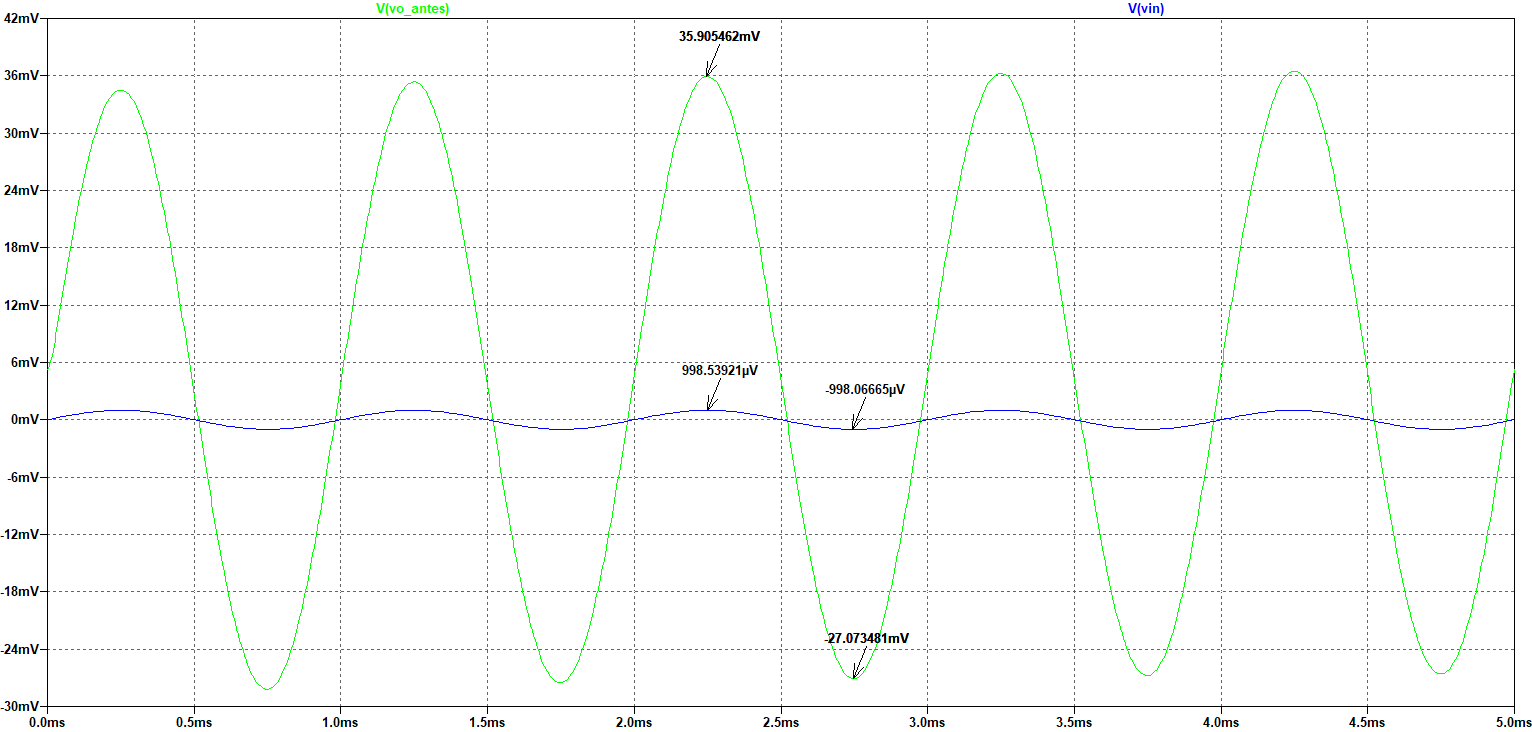
\includegraphics[width=\textwidth]{Imagenes/sim_basecomun_1m.png}
                  \caption{Simulación del voltaje de salida y entrada del amplificador base en tiempo con un $V_{in}=1mV_p$ en modo común.}
                  \label{fig:sim_basecomun_1m}
                \end{figure}

                \begin{align*}
                  A_c & =\dfrac{35.905462m-(-27.073481m)}{998.53921\mu-(-998.06665\mu)} \\[0.2cm]
                  A_c & =31.54                                                          \\[0.2cm]
                \end{align*}

                Nos da una ganancia aproximada a la calculada, por hallarse en la zona activa, verificando de esa manera que hemos hecho unos cálculos teóricos adecuados.

                Cada uno de los resultados pueden compararse con la tabla \ref{tab:dinamico_base}.

          \item  \textbf{Impedancia de entrada modo Diferencial}

                Haremos uso de la ecuación \ref{eqn:zd}, tras la simulación usar los valores dados por ello.

                \begin{figure}[H]
                  \centering
                  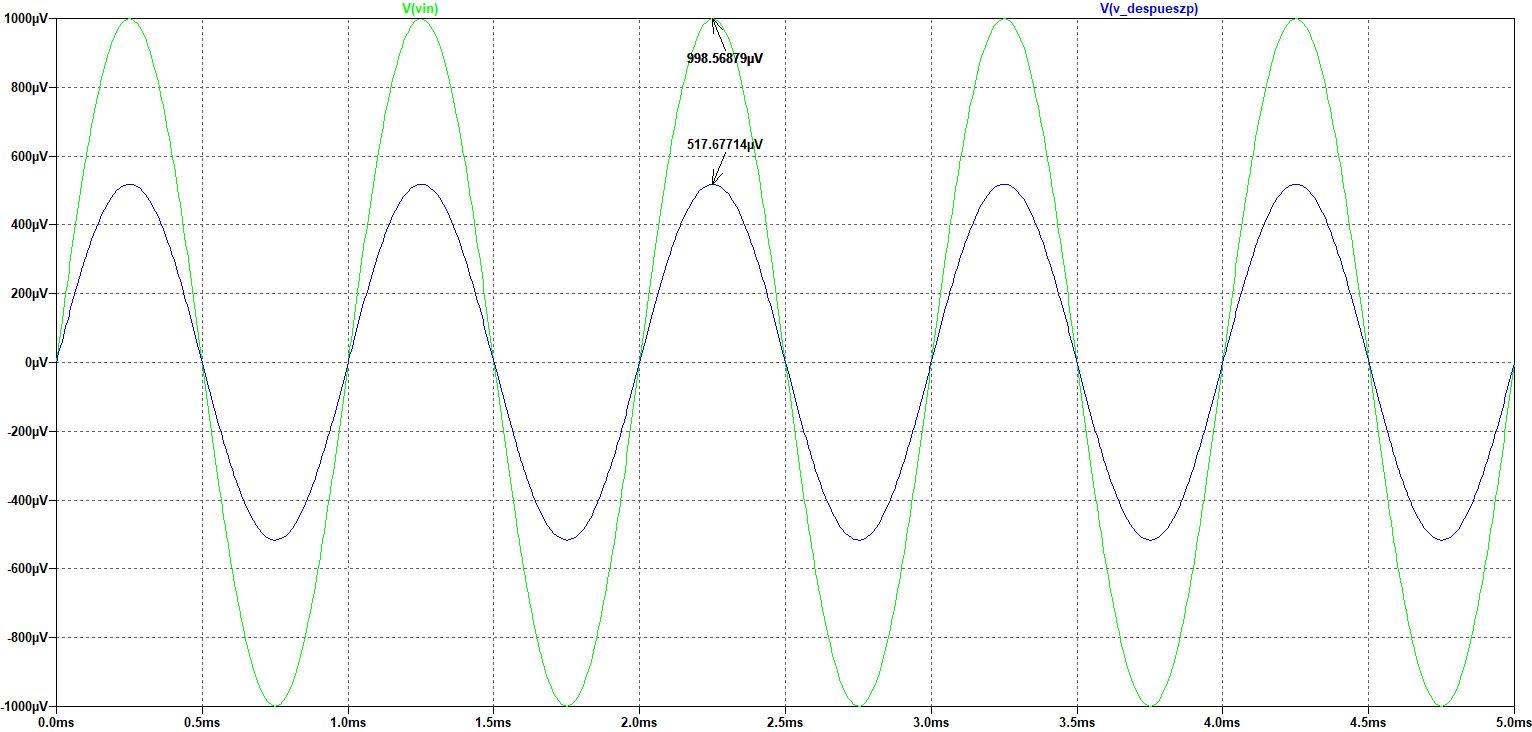
\includegraphics[width=\textwidth]{Imagenes/sim_base_zd.png}
                  \caption{Simulación del voltaje de entrada y después de $Z_p$ en modo común, para hallar $Z_d$.}
                  \label{fig:sim_base_zd}
                \end{figure}

                \begin{align*}
                  Z_{d} & =\dfrac{V_{despues\_de\_Z\_p}Z_p}{V_{in}-V_{despues\_de\_Z\_p}} \\[0.2cm]
                  Z_{d} & =\dfrac{517.67714\mu(42k)}{998.56879\mu-517.67714\mu}           \\[0.2cm]
                  Z_{d} & =45.212k\ohm                                                    \\[0.2cm]
                \end{align*}

          \item  \textbf{Impedancia de entrada modo Común}

                Haremos uso de la ecuación \ref{eqn:zc}, tras la simulación usar los valores dados por ello.


                \begin{figure}[H]
                  \centering
                  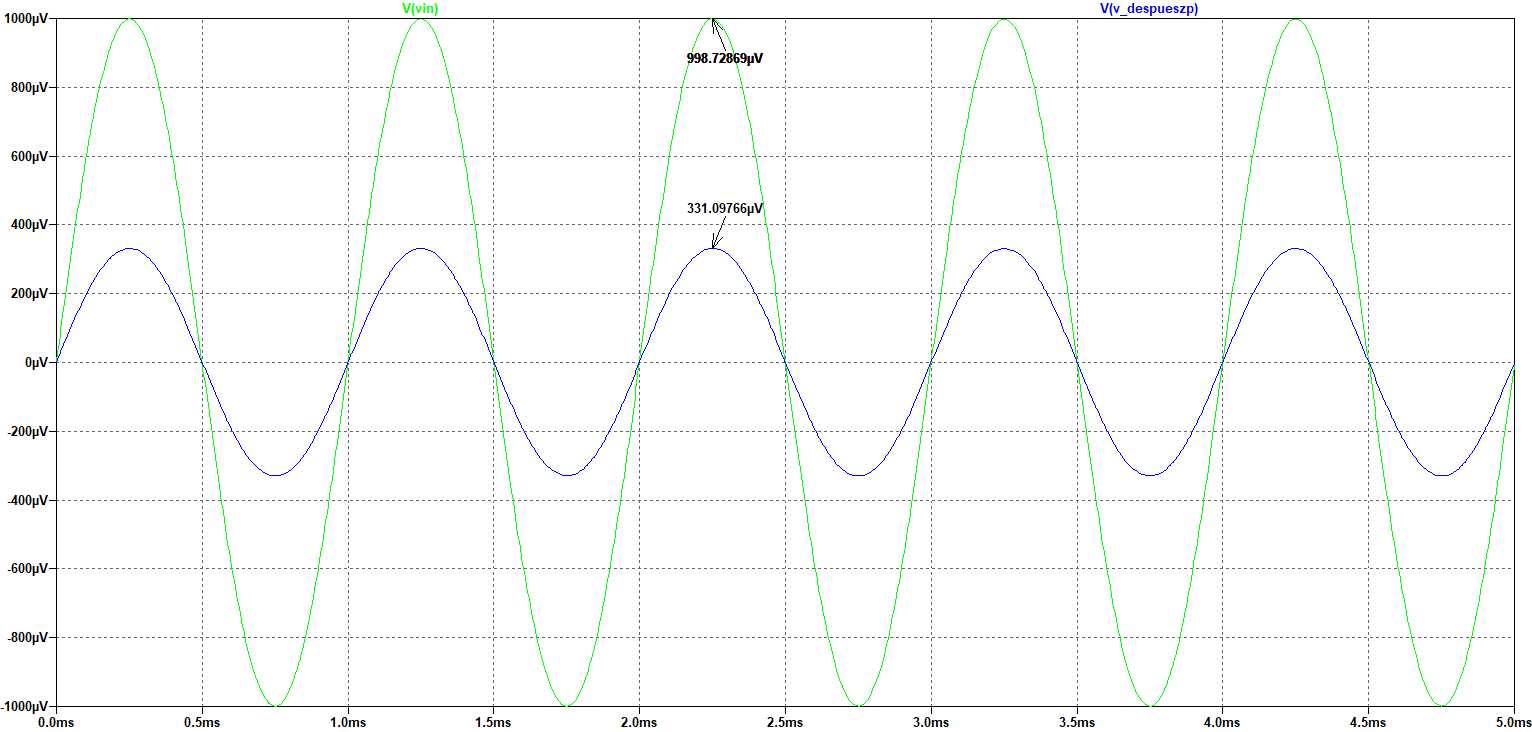
\includegraphics[width=\textwidth]{Imagenes/sim_base_zc.png}
                  \caption{Simulación del voltaje de entrada y después de $Z_p$ en modo común, para hallar $Z_c$.}
                  \label{fig:sim_base_zc}
                \end{figure}

                \begin{align*}
                  Z_{c} & =2\dfrac{V_{despues\_de\_Z\_p}Z_p}{V_{in}-V_{despues\_de\_Z\_p}} \\[0.2cm]
                  Z_{c} & =2\dfrac{517.67714\mu(50k)}{998.56879\mu-517.67714\mu}           \\[0.2cm]
                  Z_{c} & =49.6k\ohm                                                       \\[0.2cm]
                \end{align*}

          \item  \textbf{Impedancia de salida}

                En este apartado, se va a establecer la impedancia de salida con la ecuación \ref{eqn:zo}, pero bajo las simulaciones realizadas previamente para la metodología adecuada del laboratorio.

                \begin{figure}[H]
                  \centering
                  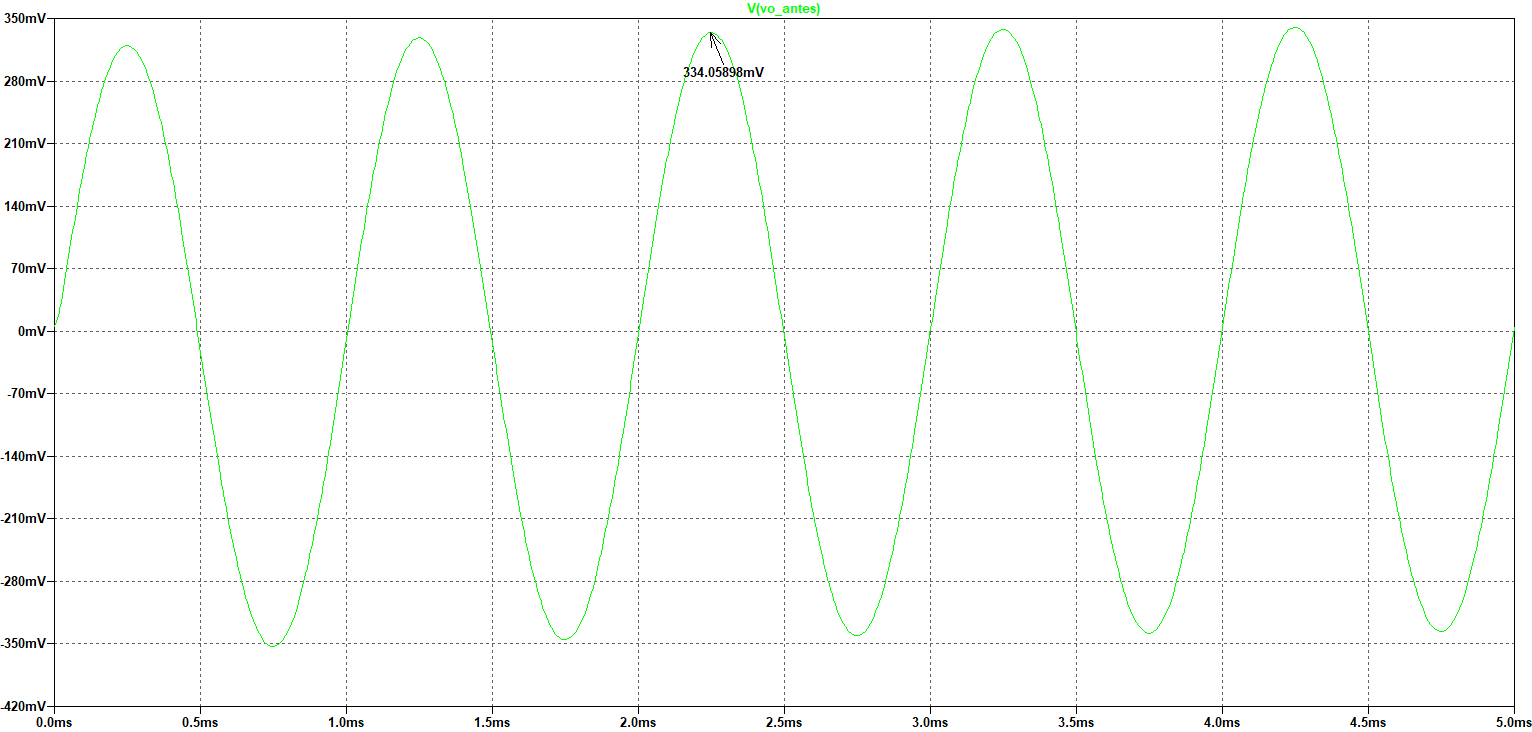
\includegraphics[width=\textwidth]{Imagenes/vosc_base.png}
                  \caption{Simulación del voltaje de salida sin carga del amplificador base en tiempo para hallar la impedancia de salida.}
                  \label{fig:vosc_base}
                \end{figure}

                En la figura \ref{fig:vosc_base}, se visualiza el voltaje de salida sin carga, ahora se usara el valor de la simulación de la figura \ref{fig:vocc_base}, y hallar la impedancia de salida.

                \begin{figure}[H]
                  \centering
                  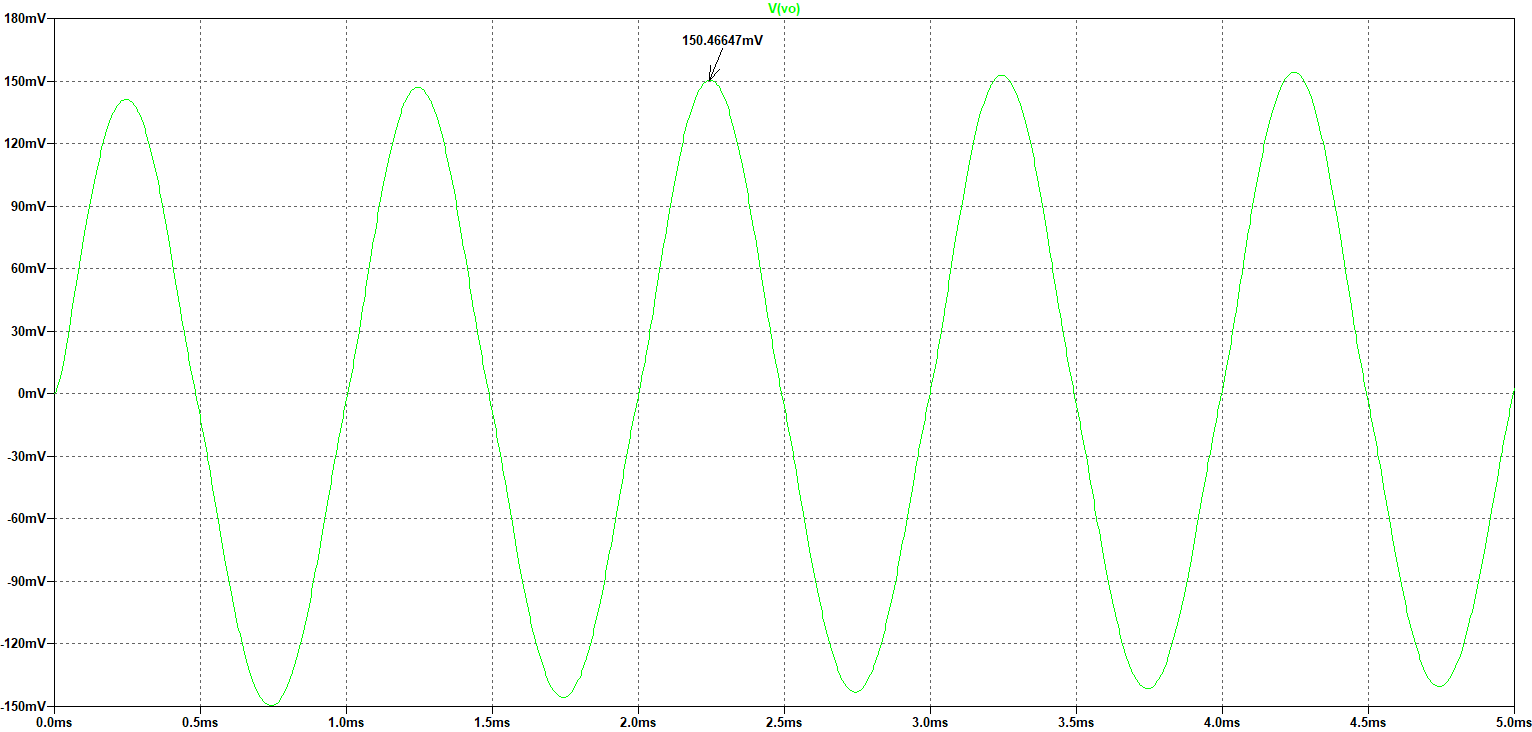
\includegraphics[width=\textwidth]{Imagenes/vocc_base.png}
                  \caption{Simulación del voltaje de salida con carga del amplificador base en tiempo para hallar la impedancia de salida.}
                  \label{fig:vocc_base}
                \end{figure}

                \begin{align*}
                  Z_{out} & =\dfrac{(V_{sin\_carga}-V_{con\_carga})Z_p}{V_{con\_carga}} \\[0.2cm]
                  Z_{out} & =\dfrac{(334.05898m-150.46647m)30}{150.46647m}              \\[0.2cm]
                  Z_{out} & =36.6\ohm                                                   \\[0.2cm]
                \end{align*}

        \end{itemize}

        \begin{table}[H]
          \centering
          \begin{tabular}{|c|c|c|c|c|}
            \hline
            $\mathbf{A_d}$ & $\mathbf{A_c}$ & $\mathbf{Z_{d}[\ohm]}$ & $\mathbf{Z_{c}[\ohm]}$ & $\mathbf{Z_{out} [\ohm]}$ \\ \hline
            5.7            & 5.6            & 45.212k                & 49.593k                & 36.6                      \\ \hline
          \end{tabular}
          \captionsetup{labelfont={bf}}
          \caption{Ganancia e impedancias simuladas del amplificador base con un $V_{in}=1V_p$}
          \label{tab:dinamico_base_sim1}
        \end{table}

        \begin{table}[H]
          \centering
          \begin{tabular}{|c|c|c|c|c|}
            \hline
            $\mathbf{A_d}$ & $\mathbf{A_c}$ & $\mathbf{Z_{d}[\ohm]}$ & $\mathbf{Z_{c}[\ohm]}$ & $\mathbf{Z_{out} [\ohm]}$ \\ \hline
            328.86         & 34.54          & 45.212k                & 49.593k                & 36.6                      \\ \hline
          \end{tabular}
          \captionsetup{labelfont={bf}}
          \caption{Ganancia e impedancias simuladas del amplificador base con un $V_{in}=1mV_p$}
          \label{tab:dinamico_base_sim1m}
        \end{table}

\end{enumerate}


\subsection{Parte 4. Respuesta en frecuencia}

\begin{enumerate}
  \item \textbf{Para el amplificador base (figura \ref{fig:amplificador_base}), determine: Punto
          de operación de los elementos activos y modelo dinámico del amplificador, incluyendo su respuesta en frecuencia.}

        Los datos de los puntos de operación y modelo dinámico se encuentran en las tablas \ref{tab:ptos_ed}, \ref{tab:ptos_ei}, \ref{tab:ptos_ep} y \ref{tab:dinamico_base}.

        Se hará énfasis en su respuesta en frecuencia

        \subsubsection{Frecuencia de corte inferior}

        \begin{itemize}
          \item $\mathbf{C_1}$ y $\mathbf{C_3}$

                Se toman $C_1$ y $C_3$ como iguales, debido a que es el mismo recorrido de corriente en la etapa diferencial, uno es de acople y el otro de desacople.

                Se aplica el método de respuesta en frecuencia para corte inferior, se obtiene el siguiente circuito de la figura \ref{fig:c1}
                \begin{figure}[H]
                  \centering
                  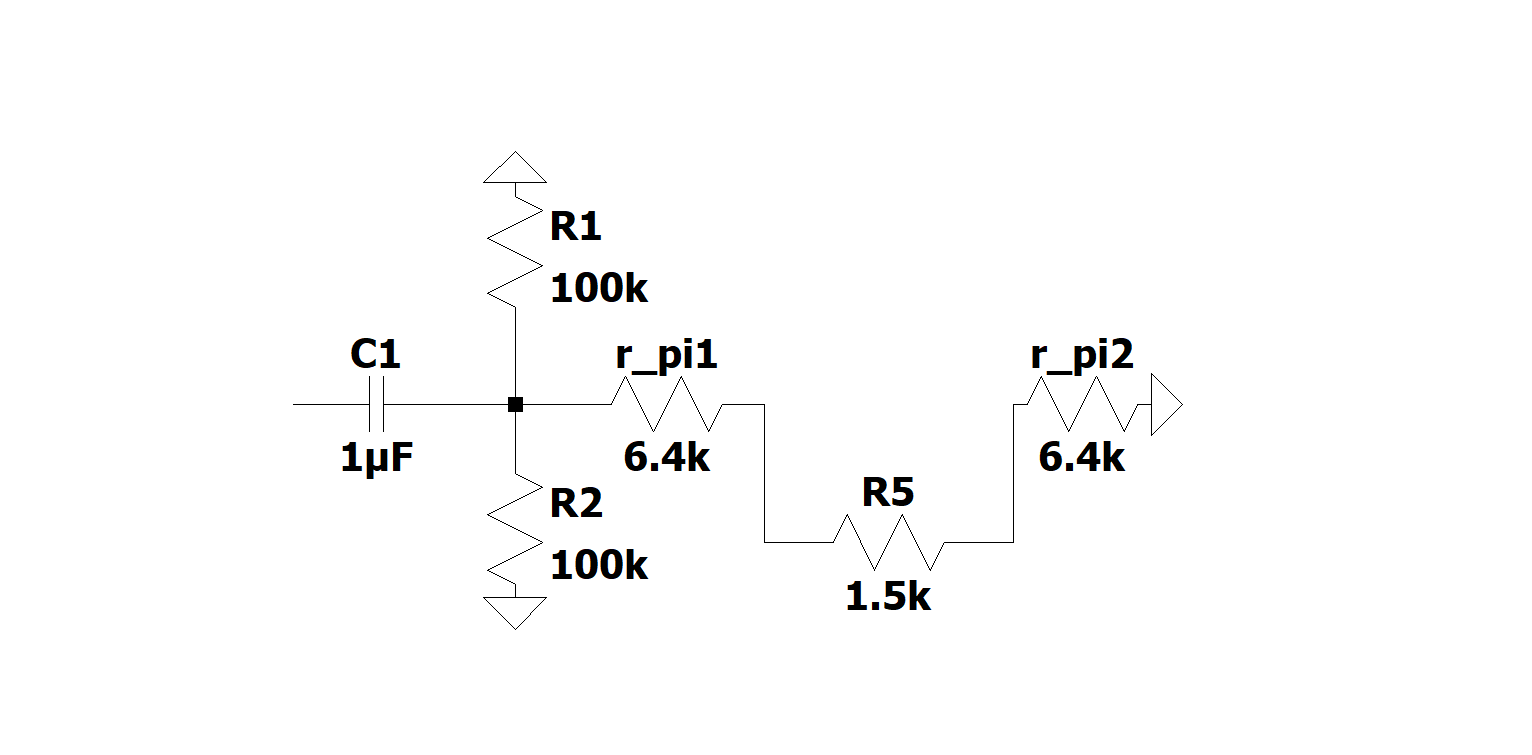
\includegraphics[width=12cm]{Imagenes/c1.png}
                  \caption{Diagrama esquemático al aplicar el análisis de frecuencia de corte inferior a $C_1$.}
                  \label{fig:c1}
                \end{figure}

                Se halla la $Z_{eq}$ del circuito de la figura \ref{fig:c1}, dando como resultado lo siguiente,

                Aplicando la ecuación \ref{eqn:wl}.

                \begin{align*}
                  w_{p_1} & =w_{p_3}=\dfrac{1}{C_1Z_{eq}}                                                                                    \\[0.2cm]
                  w_{p_1} & =\dfrac{1}{C_1[R_1||R_2||(r_{\pi_1}+(g_{m_1}r_{\pi_1}+1)\left(R_5+\dfrac{r_{\pi_2}}{g_{m_2}r_{\pi_2}+1}\right)]} \\[0.2cm]
                  w_{p_1} & =\dfrac{1}{C_1[R_1||R_2||(2r_{\pi_1}+(g_{m_1}r_{\pi_1}+1)\left(R_5\right)]}                                      \\[0.2cm]
                  w_{p_1} & =w_{p_3}= \SI{24.18}{\radian\per\second}                                                                         \\[0.2cm]
                  f_{L_1} & =f_{L_3}= \SI{3.85}{\hertz}                                                                                      \\[0.2cm]
                \end{align*}

          \item $\mathbf{C_2}$

                \begin{figure}[H]
                  \centering
                  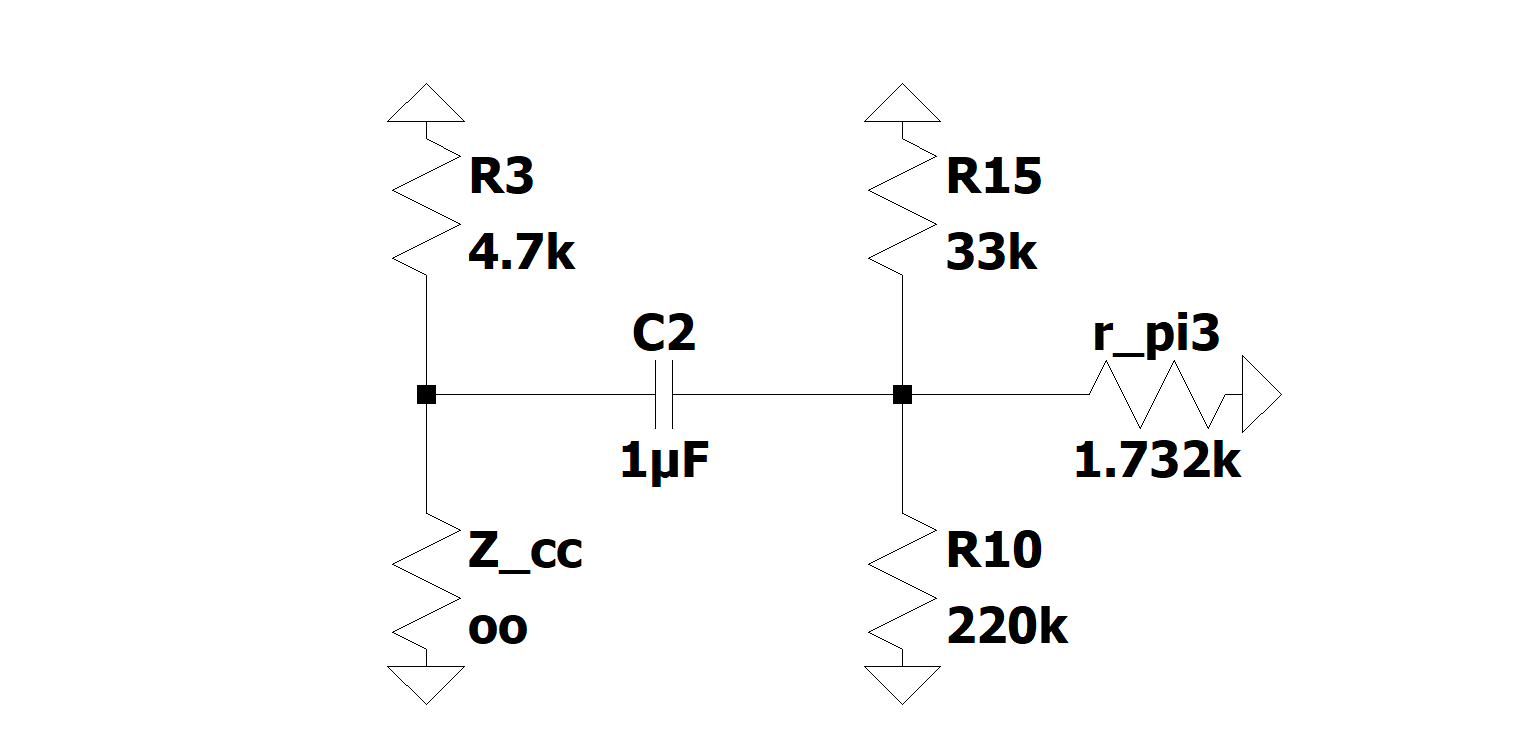
\includegraphics[width=12cm]{Imagenes/c2.png}
                  \captionsetup{labelfont={bf}}
                  \caption{Diagrama esquemático al aplicar el análisis de frecuencia de corte inferior a $C_2$.}
                  \label{fig:c2}
                \end{figure}

                Se halla la $Z_{eq}$ del circuito de la figura \ref{fig:c2}, dando como resultado lo siguiente,

                \begin{align*}
                  w_{p_2} & =\dfrac{1}{C_2Z_{eq}}                            \\[0.2cm]
                  w_{p_2} & =\dfrac{1}{C_2[R_3+(R_{15}||R_{10}||r_{\pi_3})]} \\[0.2cm]
                  w_{p_2} & = \SI{157.9}{\radian\per\second}                 \\[0.2cm]
                  f_{L_2} & = \SI{25.13}{\hertz}                             \\[0.2cm]
                \end{align*}

          \item $\mathbf{C_5}$

                \begin{figure}[H]
                  \centering
                  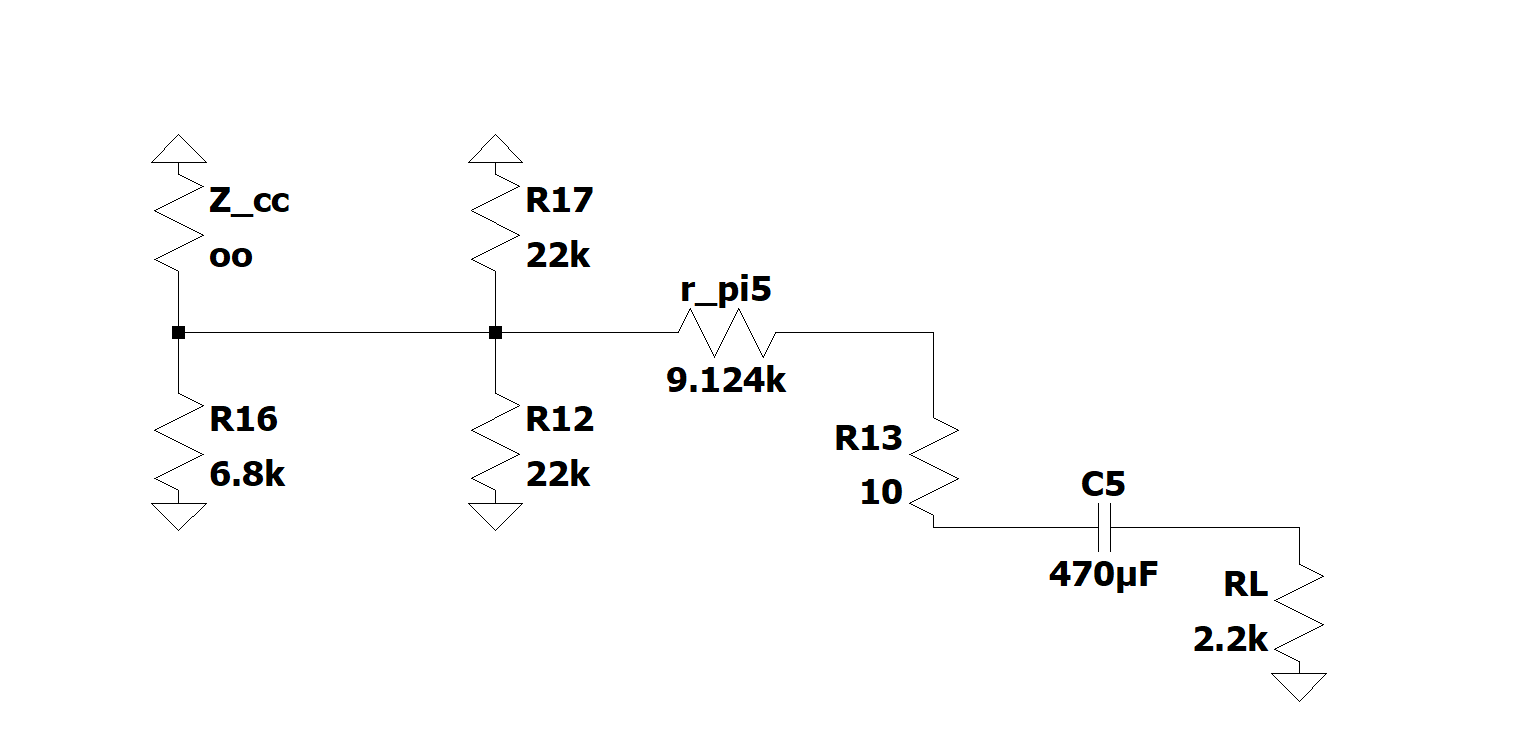
\includegraphics[width=12cm]{Imagenes/c5.png}
                  \captionsetup{labelfont={bf}}
                  \caption{Diagrama esquemático al aplicar el análisis de frecuencia de corte inferior a $C_5$.}
                  \label{fig:c5}
                \end{figure}

                Se halla la $Z_{eq}$ del circuito de la figura \ref{fig:c5}, dando como resultado lo siguiente,

                \begin{align*}
                  w_{p_5} & =\dfrac{1}{C_5Z_{eq}}                                                                               \\[0.2cm]
                  w_{p_5} & =\dfrac{1}{C_5[R_L+R_{13}+\dfrac{r_{\pi_5}+R_{17}||R_{12}||R_{16}||Z_{CCQ_3}}{g_{m_5}r_{\pi_5}+1}]}
                \end{align*}


                En este caso, para $Z_{CCQ_3}$ que es la impedancia vista desde el colector hacia el transistor, se facilita la obtención del valor, a través del transistor completamente cargado, donde se obtiene la siguiente ecuación:

                \begin{gather*}
                  Z_{CCQ_3}=r_o \left[\dfrac{r_{\pi}+Z_B+\left(g_mr_{\pi}+1+\dfrac{r_{\pi}+Z_B}{r_o}\right)Z_E}{Z_E+Z_B+r_{\pi}}\right]
                \end{gather*}

                Donde, $Z_B$, es la impedancia vista desde la base y $Z_E$, es la impedancia vista desde el emisor.

                Como se puede observar, $Z_E=0$ por el condensador, por ende, la ecuación generada por el transistor completamente cargado solo nos quedaría $Z_{CCQ_3}=r_o$, de esa manera se obtiene la siguiente frecuencia de $C_5$
                \begin{align*}
                  w_{p_5} & =\dfrac{1}{C_5[R_L+R_{13}+\dfrac{r_{\pi_5}+R_{17}||R_{12}||R_{16}||r_{o_3}}{g_{m_5}r_{\pi_5}+1}]}
                  w_{p_5} & = \SI{0.096}{\radian\per\second}                                                                  \\[0.2cm]
                  f_{L_5} & = \SI{15.31}{\milli\hertz}                                                                        \\[0.2cm]
                \end{align*}
                \newpage
          \item $\mathbf{C_6}$

                \begin{figure}[H]
                  \centering
                  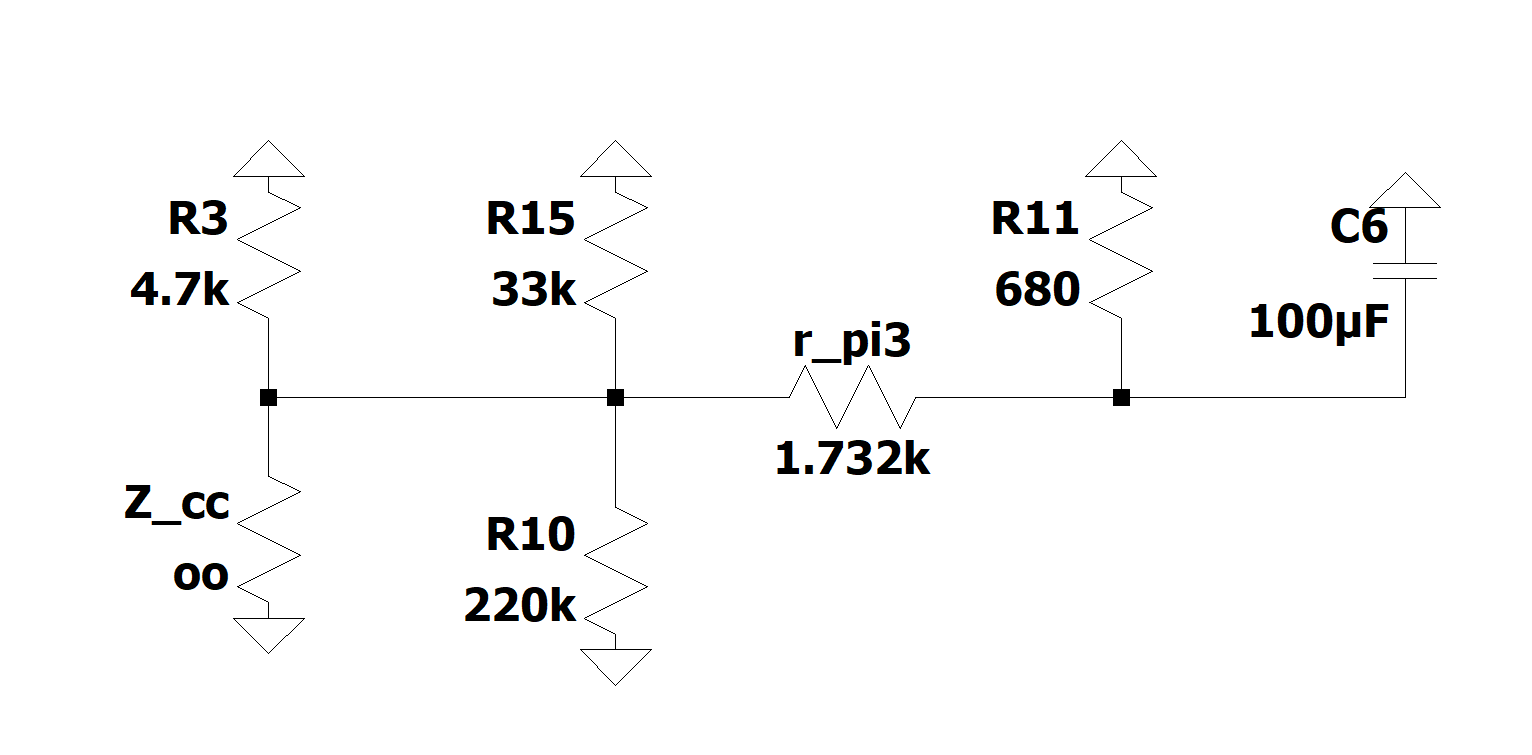
\includegraphics[width=12cm]{Imagenes/c6.png}
                  \captionsetup{labelfont={bf}}
                  \caption{Diagrama esquemático al aplicar el análisis de frecuencia de corte inferior a $C_6$.}
                  \label{fig:c6}
                \end{figure}

                Se halla la $Z_{eq}$ del circuito de la figura \ref{fig:c6}, dando como resultado lo siguiente,

                \begin{align*}
                  w_{p_6} & =\dfrac{1}{C_6Z_{eq}}                                                                             \\[0.2cm]
                  w_{p_6} & =\dfrac{1}{C_6[R_{11}||\left(\dfrac{r_{\pi_3}+R_{15}||R_{10}||R_{3}}{g_{m_3}r_{\pi_3}+1}\right)]} \\[0.2cm]
                  w_{p_6} & = \SI{277.22}{\radian\per\second}                                                                 \\[0.2cm]
                  f_{L_6} & = \SI{44.121}{\hertz}                                                                             \\[0.2cm]
                \end{align*}

          \item $\mathbf{C_7}$

                \begin{figure}[H]
                  \centering
                  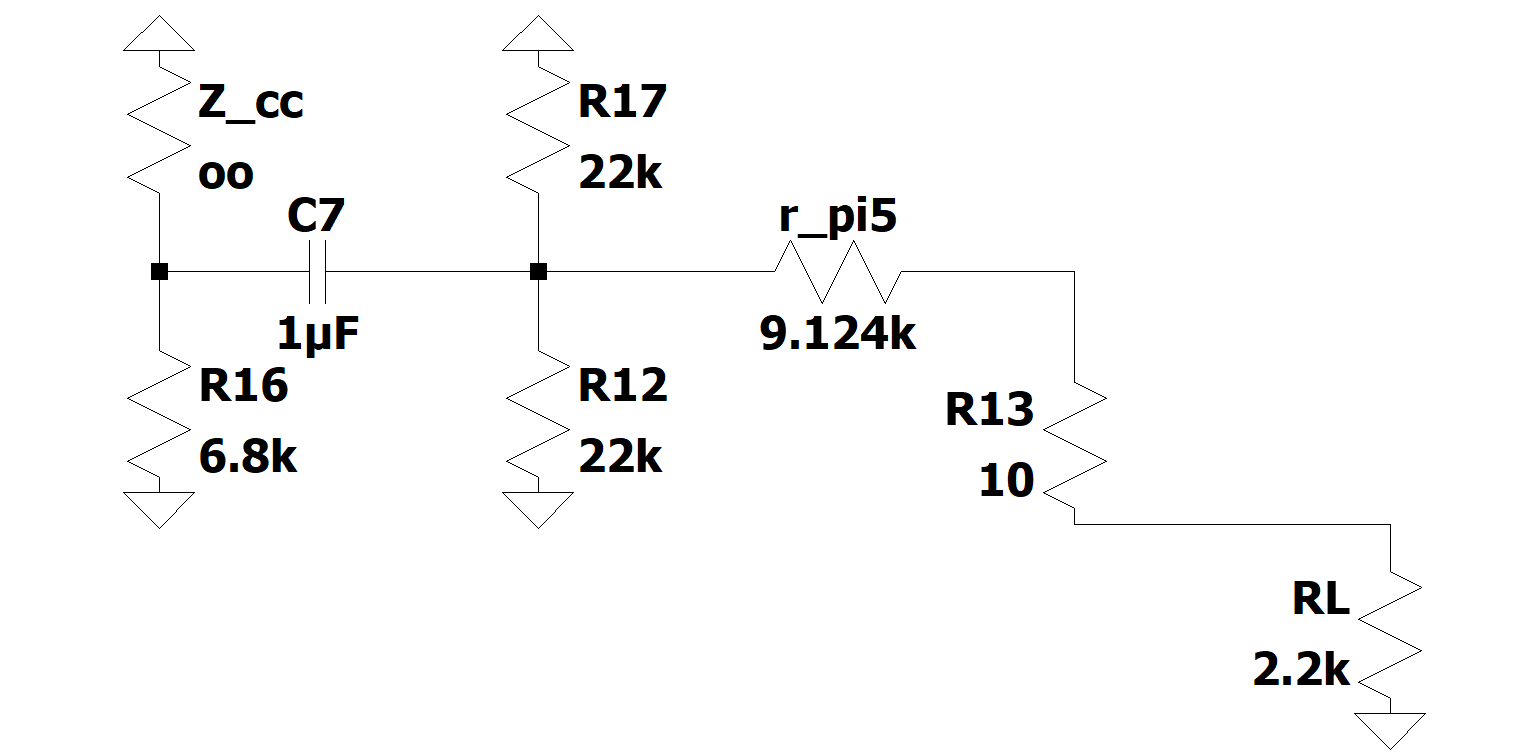
\includegraphics[width=12cm]{Imagenes/c7.png}
                  \captionsetup{labelfont={bf}}
                  \caption{Diagrama esquemático al aplicar el análisis de frecuencia de corte inferior a $C_7$.}
                  \label{fig:c7}
                \end{figure}

                Se halla la $Z_{eq}$ del circuito de la figura \ref{fig:c7}, dando como resultado lo siguiente,

                \begin{align*}
                  w_{p_7} & =\dfrac{1}{C_7Z_{eq}}                                                                \\[0.2cm]
                  w_{p_7} & =\dfrac{1}{C_7[R_{16}+R_{17}||R_{12}||(r_{\pi_5}+(g_{m_5}r_{\pi_5}+1)(R_{13}+R_L))]} \\[0.2cm]
                  w_{p_7} & = \SI{57.28}{\radian\per\second}                                                     \\[0.2cm]
                  f_{L_7} & = \SI{9.12}{\hertz}                                                                  \\[0.2cm]
                \end{align*}

                Como se pueden observar en los resultados, el capacitor mas dominante es el $\mathbf{C_6}$ siendo este el de bypass quien nos permite una mayor ganancia, teniendo sentido en los cálculos teóricos
        \end{itemize}

        \subsubsection{Frecuencia de corte superior}
        \begin{itemize}
          \item $\mathbf{C_4}$

                En este apartado tomaremos en cuenta el teorema de Miller y el análisis de frecuencia de corte superior, las ecuaciones que se usaran son \ref{eqn:C_eq} y \ref{eqn:wh}, bajo el modelo pi de altas frecuencias, como se muestra en la figura \ref{fig:c4}

                \begin{figure}[H]
                  \centering
                  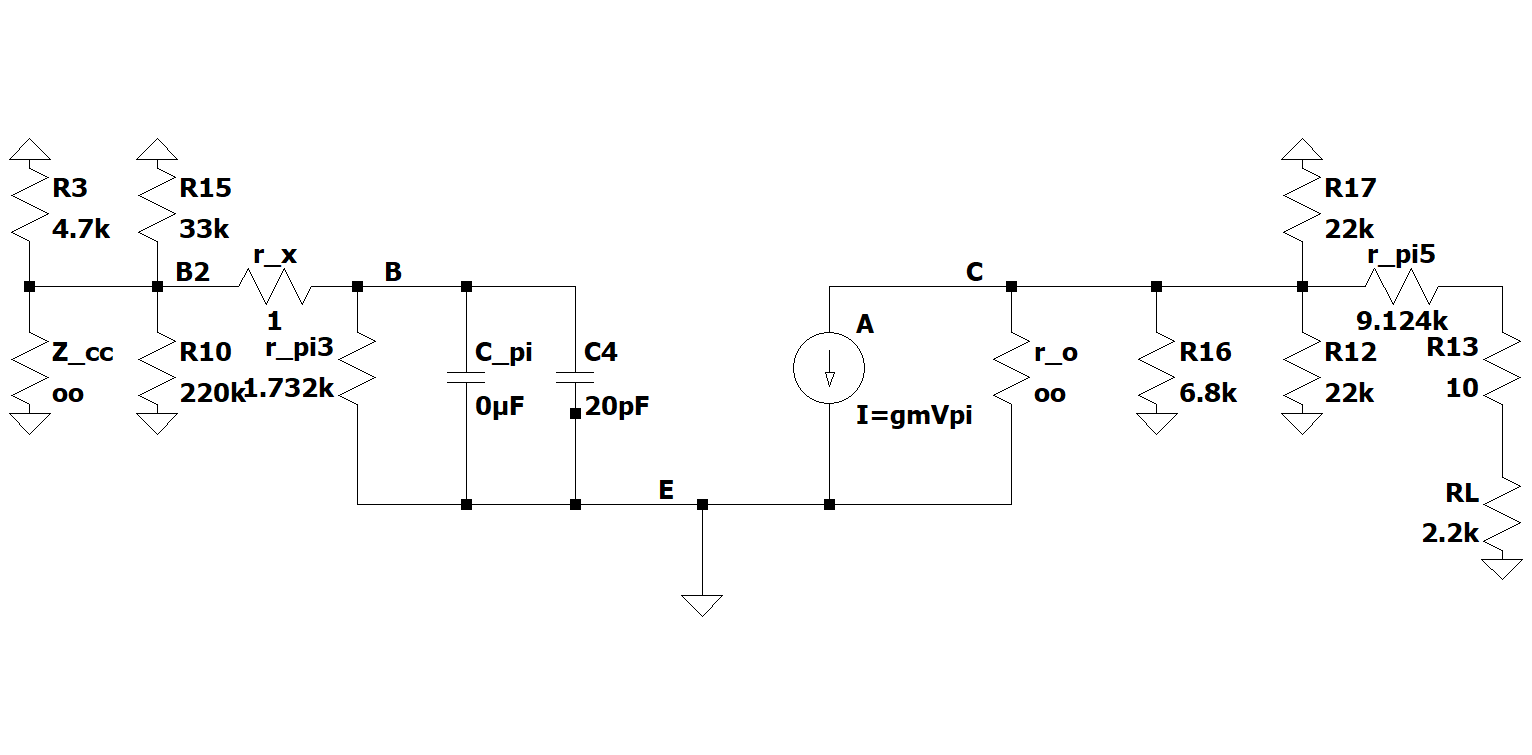
\includegraphics[width=\textwidth]{Imagenes/c4.png}
                  \captionsetup{labelfont={bf}}
                  \caption{Diagrama esquemático al aplicar el análisis de frecuencia de corte superior a $C_4$, aplicando Teorema de Miller.}
                  \label{fig:c4}
                \end{figure}

                \begin{align*}
                  \mathbf{C_{eq}} = C_{\pi} + C_{\mu}(1+g_mZ_{out})
                \end{align*}

                En este caso, se toma en cuenta el apartado de Anexos \ref{sec:anexos} donde se verifica que el transistor 2n3906 (PNP), el datasheet indica que $C_{\pi}=10 \, pF$ y $C_{\mu}=4.5 \, pF$, por lo tanto, se tiene que $C_{eq}$ es,

                \begin{align*}
                  \mathbf{C_{eq}} =C_{\pi}+ (C_{\mu}+C_4)(1+g_mZ_{out})
                \end{align*}

                Ahora, se halla $Z_{out}$ y sustituimos en \ref{eqn:C_eq},

                \begin{align*}
                  Z_{out} & =Z_{CCQ_3}||R_{16}||R_{17}||R_{12}||(r_{\pi_5}+(g_{m_5}r_{\pi_5}+1)(R_{13}+R_L))                                  \\[1cm]
                  C_{eq}  & =C_{\pi}+ (C_{\mu} + C_{4})(1+g_m[r_{o_3}||R_{16}||R_{17}||R_{12}||(r_{\pi_5}+(g_{m_5}r_{\pi_5}+1)(R_{13}+R_L))])
                \end{align*}

                Se toma en este caso, la ecuación \ref{eqn:rx}, donde se obtiene el valor de la resistencia de difusión;

                \begin{gather}
                  r_x=\dfrac{25.581 m}{2.253m}=11.35 \approx 11 \ohm
                \end{gather}


                luego se halla $Z_{in}$ y sustituimos en la ecuación \ref{eqn:wh}

                \begin{align*}
                  Z_{in} & =r_{\pi_3}||(r_{x}+(R_{15}||R_{10}||R_3))                                                                                                                                     \\[1cm]
                  w_{H}  & =\dfrac{1}{C_{eq}Z_{in}}                                                                                                                                                      \\[0.2cm]
                  w_{H}  & = \dfrac{1}{C_{\pi} + (C_{\mu} + C_{4})(1+g_{m_3}[r_{o_3}||R_{16}||R_{17}||R_{12}||(r_{\pi_5}+(g_{m_5}r_{\pi_5}+1)(R_{13}+R_L))]) [r_{\pi_3}||(r_{x}+(R_{15}||R_{10}||R_3))]} \\[0.2cm]
                  w_{H}  & =\SI{98.615}{\kilo\radian\per\second}                                                                                                                                         \\[0.2cm]
                  f_{H}  & =\SI{15.695}{\kilo\hertz}                                                                                                                                                     \\[0.2cm]
                \end{align*}

        \end{itemize}


        \begin{table}[H]
          \centering
          \begin{tabular}{|c|c|c|c|c|}
            \hline
            \textbf{Capacitores} & \boldmath{$\mathbf{w_L}$ (\si{\radian\per\second})} & \boldmath{$\mathbf{f_L}$ (\si{\hertz})} & \boldmath{$\mathbf{w_H}$ (\si{\radian\per\second})} & \boldmath{$\mathbf{f_H}$ (\si{\hertz})} \\\hline
            1                    & 24.18                                               & 3.85                                    & -                                                   & -                                       \\\hline
            2                    & 157.9                                               & 25.13                                   & -                                                   & -                                       \\\hline
            3                    & 24.18                                               & 3.85                                    & -                                                   & -                                       \\\hline
            4                    & -                                                   & -                                       & 98.615k                                             & 15.695k                                 \\\hline
            5                    & 0.096                                               & 15.31m                                  & -                                                   & -                                       \\\hline
            6                    & 277.22                                              & 44.121                                  & -                                                   & -                                       \\\hline
            7                    & 57.28                                               & 9.12                                    & -                                                   & -                                       \\\hline
          \end{tabular}
          \captionsetup{labelfont={bf}}
          \caption{Calculo teórico en el análisis de frecuencia de corte inferior y superior}
          \label{tab:frecuencias}
        \end{table}

        Como se puede observar en la frecuencia de corte inferior, el más dominante es la del capacitor $C_6$, siendo este el de bypass, debido a que permite una mayor ganancia, siendo el mas dominante en la frecuencia de baja, de esta manera sabemos que esa es la frecuencia de corte inferior.

        Por otro lado, tenemos el capacitor $C_4$ que es el que afecta en la frecuencia de corte superior, generando la frecuencia de corte superior como se observa en la tabla \ref{tab:frecuenciacorte}

        \begin{table}[H]
          \centering
          \begin{tabular}{|c|c|}
            \hline
            \boldmath{$\mathbf{f_L}$ (\si{\hertz})} & \boldmath{$\mathbf{f_H}$ (\si{\hertz})} \\\hline
            44.121                                  & 15.695k                                 \\\hline
          \end{tabular}
          \captionsetup{labelfont={bf}}
          \caption{Frecuencias de corte superior e inferior teórico}
          \label{tab:frecuenciacorte}
        \end{table}

  \item \textbf{Realice la simulación del circuito con el fin de verificar los cálculos previos.}

        \begin{figure}[H]
          \centering
          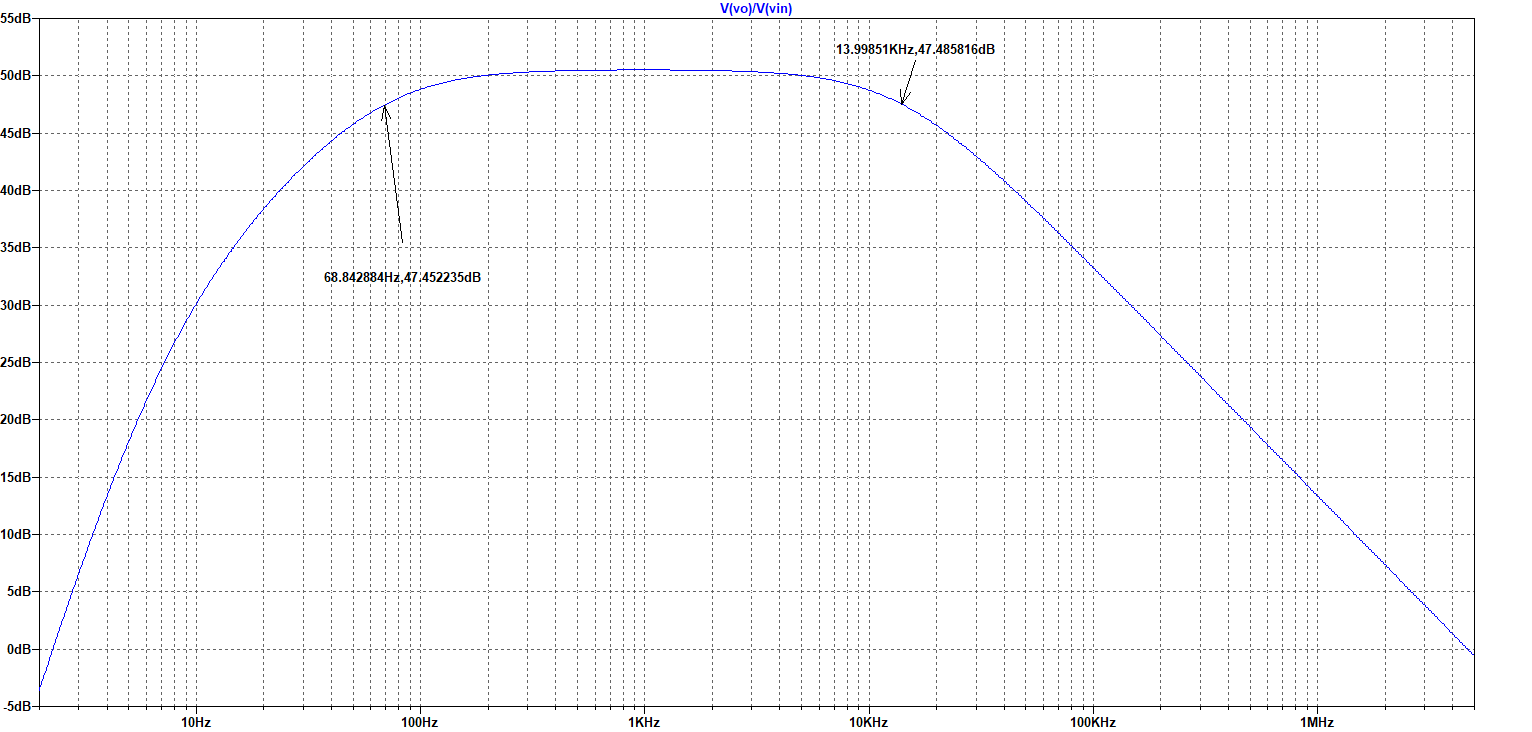
\includegraphics[width=\textwidth]{Imagenes/sim_resp_frecu.png}
          \captionsetup{labelfont={bf}}
          \caption{Simulación de la respuesta en frecuencia del amplificador base acoplando.}
          \label{fig:frecuenciacorte}
        \end{figure}

        \begin{figure}[H]
          \centering
          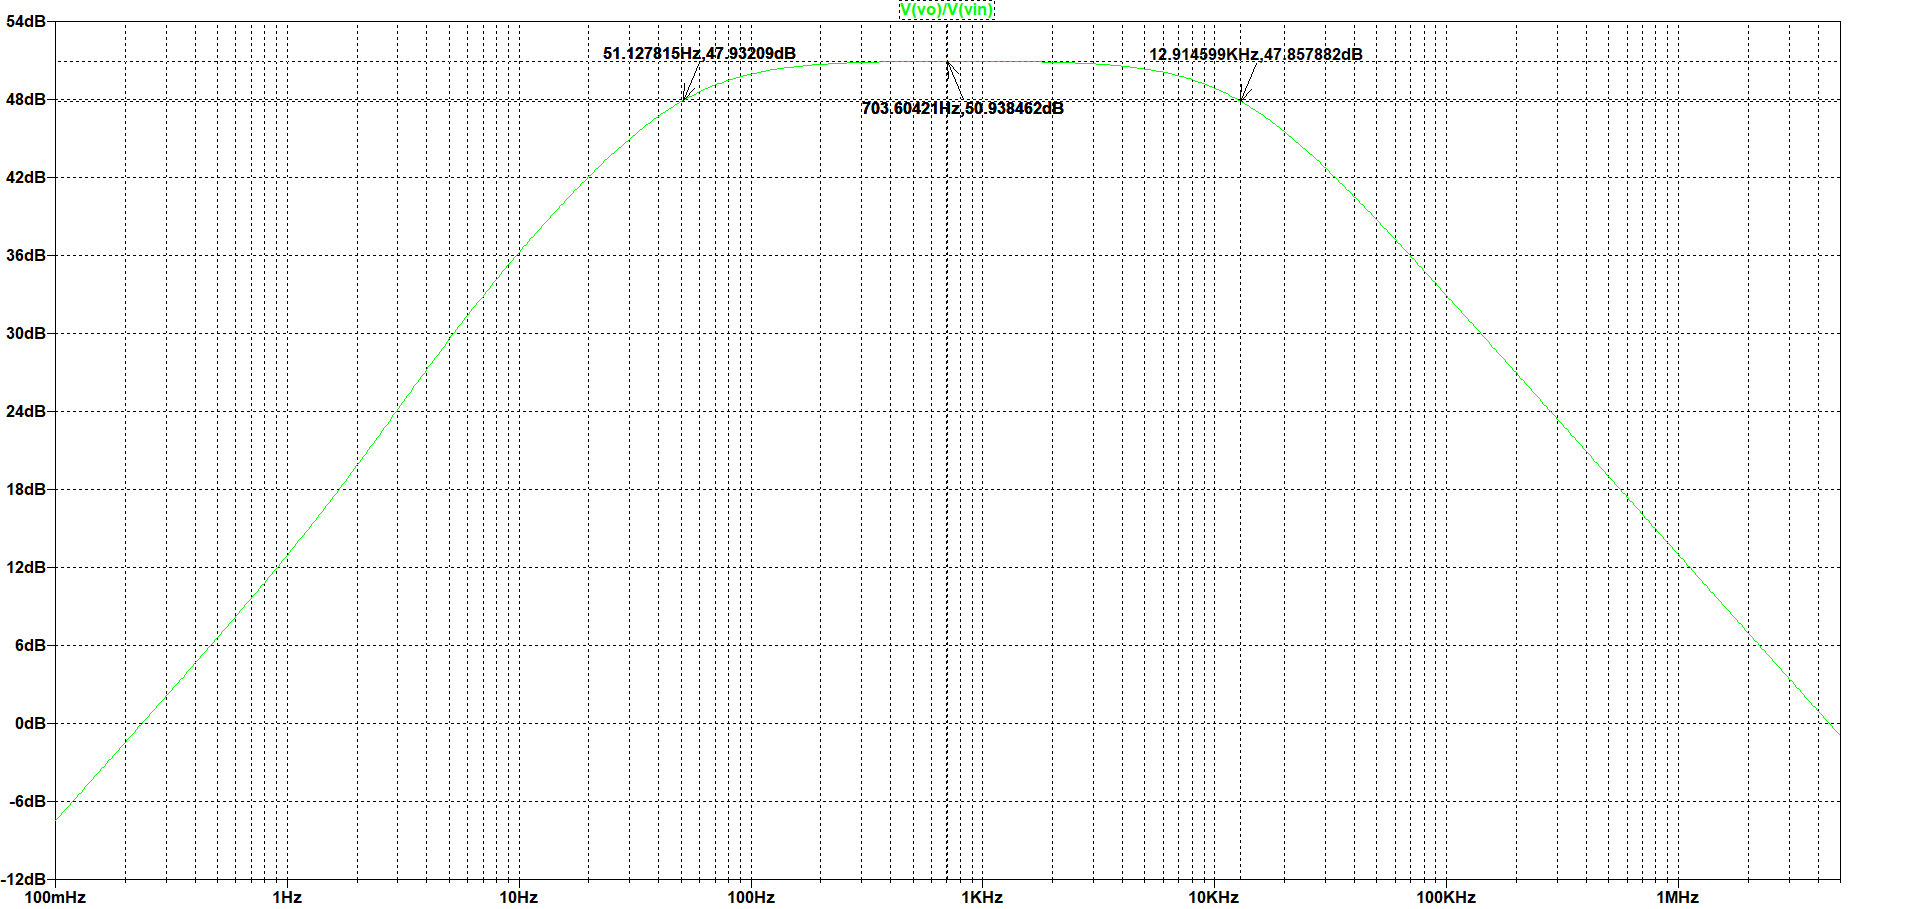
\includegraphics[width=\textwidth]{Imagenes/sim_resp_frecu_sin.png}
          \captionsetup{labelfont={bf}}
          \caption{Simulación de la respuesta en frecuencia del amplificador base sin acople de C2,C5,C7.}
          \label{fig:frecuenciacortesinacople}
        \end{figure}

        Como se puede observar los datos obtenidos de la simulación de la figura \ref{fig:frecuenciacorte} y \ref{fig:frecuenciacortesinacople}, en ambos casos se observa una ganancia aproximadamente cerca indicandonos que sea acoplado o desacoplado permitirá mantener su polarización
        obteniendo ganancias cercanas.

        Es importante recalcar que se puede hallar la frecuencia de corte total de la respuesta en frecuencia gracias a la ecuación \ref{eqn:wt}.

        \begin{align*}
          w_t & =\beta \cdot f_H         \\[0.2cm]
          w_t & =150 \cdot 15.695k       \\[0.2cm]
          w_t & =\SI{2.354}{\mega\hertz} \\[0.2cm]
        \end{align*}

        Nos da valores aproximados a los calculado, esto indica que los cálculos teóricos están bien realizados.

\end{enumerate}

\subsection{Parte 5. Realimentación}
\begin{enumerate}
  \item \textbf{Realimente negativamente el amplificador base a través de la entrada diferencial adecuada, mediante un divisor de tensión $R_f$ y $R_s$ , cuyos valores son los siguientes:}

        $$R_f=11k\ohm$$
        $$R_s=3.3k\ohm$$
        Para identificar de una manera más sencilla cual de las dos entradas de la etapa diferencial será la entrada positiva y negativa, podemos hacer el recorrido del amplificador base de la figura \ref{fig:amplificador_base}, primero desde una entrada y luego de la otra. El resultado final nos indicara si es positiva o negativa. Sin importar que este la fuente de voltaje en el nodo de la base del transistor 2. De esa manera, se tiene lo siguiente:

        Recorrido por $V_1$, que es donde tenemos la entrada de señal AC.

        Se recorre la base de $Q_1$ al colector de este mismo, que es donde se encuentra la salida de la etapa diferencial, cuando se va de base a colector la ganancia es negativa, debido a su modelo pi.

        $$A_1=-A_1$$

        Luego tenemos de base a colector de $Q_2$, que como se indico anteriormente que la ganancia sera negativa.

        $$A_2=-A_2$$

        Finalmente, tenemos $Q_3$ que va de base a emisor, que en este caso, dá una ganancia positiva.

        $$A_3=A_3$$

        Hallando la ganancia total del amplificador multietapas, dá el siguiente signo.
        $$A_V=-A_1(-A_2)A_3>0$$

        Por ende, donde se encuentra la señal de entrada es la entrada positiva del amplificador, por consiguiente, la entrada donde se encuentra la fuente negativa, es la entrada negativa. No por que posee una fuente negativa ocurre eso, sino por el estudio hecho anteriormente.

        En la figura \ref{fig:realimentadon} que se verá a continuación se tendrá el circuito realimentado por la entrada $V_2$, que seria la entrada inversora.

        \begin{figure}[H]
          \centering
          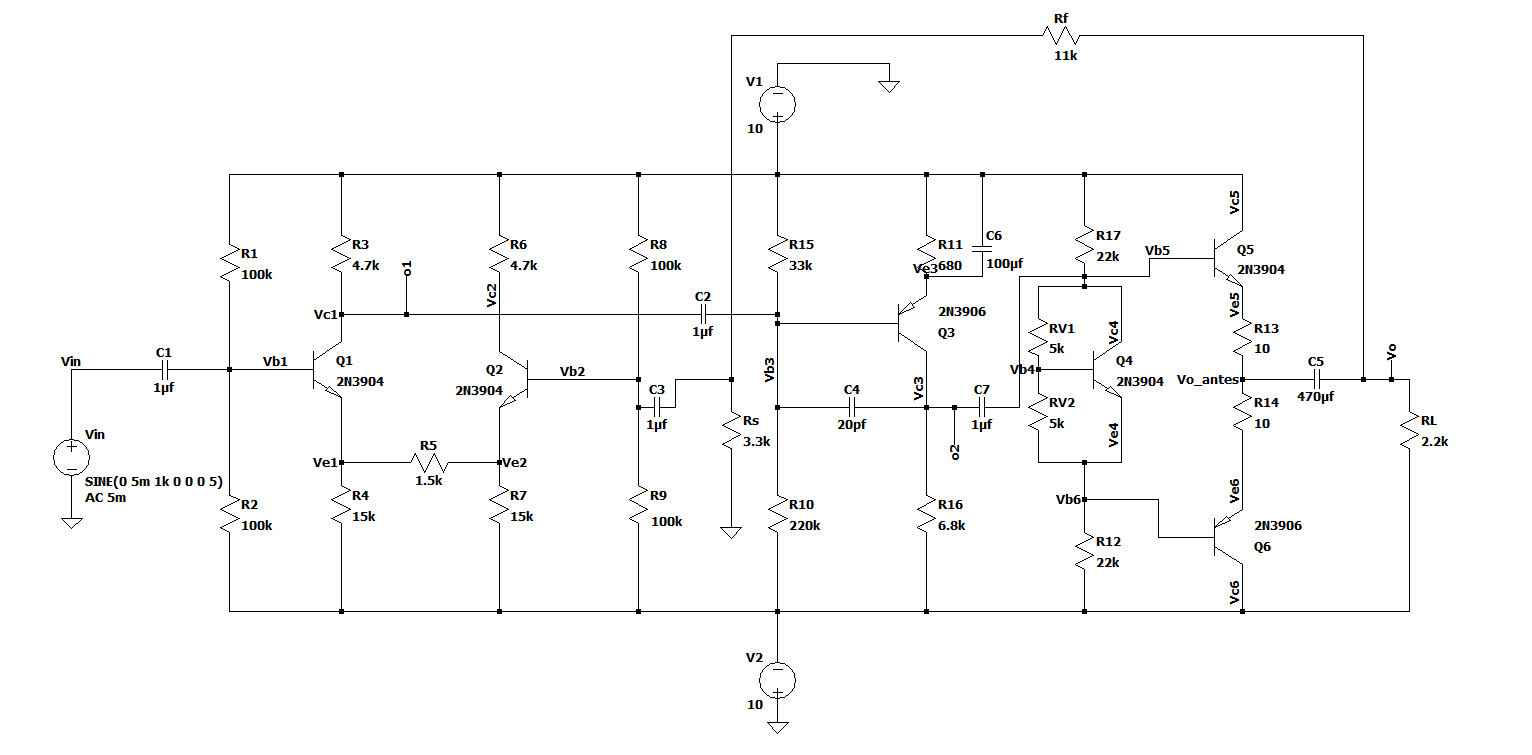
\includegraphics[width=\textwidth]{Imagenes/realimentado.png}
          \captionsetup{labelfont={bf}}
          \caption{Diagrama esquemático del amplificador base realimentado negativamente.}
          \label{fig:realimentadon}
        \end{figure}

  \item \textbf{Para el amplificador realimentado, determine: Puntos de operación de los elementos activos, el modelo dinámico del amplificador y su respuesta en frecuencia, utilizando la entrada libre del diferencial como entrada.}

        Los datos de los puntos de operación y modelo dinámico , no cambian, por ende, se encuentran en las tablas \ref{tab:ptos_ed}, \ref{tab:ptos_ei}, \ref{tab:ptos_ep} y \ref{tab:dinamico_base} .

        Sin embargo su respuesta en frecuencia si cambian, se realizará su estudio a continuación.

        \subsubsection{Respuesta en frecuencia}

        Se tomarán en cuenta las ecuaciones \ref{eqn:afb}, \ref{eqn:whfb} y \ref{eqn:wlfb}


        \begin{align*}
          A_{fb}     & =1+\dfrac{R_f}{R_s}= 4.33                                   \\[1cm]
          \beta      & =\dfrac{A_{fb}-A_{fm}}{A_{fb} A_{fm}}=-0.23                 \\[1cm]
          w_{L_{fb}} & =\dfrac{w_L}{\beta A_{fm}}                                  \\[0.2cm]
          w_{L_{fb}} & =\dfrac{277.22}{0.23(378.84)}=\SI{3.18}{\radian\per\second} \\[0.2cm]
          f_{L_{fb}} & =\SI{0.506}{\hertz}                                         \\[1cm]
          w_{H_{fb}} & =w_H(\beta A_{fm})=\SI{8.593}{\mega\radian\per\second}      \\[0.2cm]
          f_{H_{fb}} & =\SI{1.37}{\mega\hertz}                                     \\[1cm]
        \end{align*}

        \textbf{Impedancia de entrada en realimentación}

        Haciendo uso de las ecuaciones \ref{eqn:zinfb} y \ref{eqn:zofb}, tenemos lo siguiente:

        \begin{align*}
          Z_{in} & =Z_d\left(1 +\dfrac{A_{fm}}{A_{fb}}\right)      \\[0.2cm]
          Z_{in} & =41.36k\left(1 +\dfrac{A_{378.84}}{4.33}\right) \\[0.2cm]
          Z_{in} & =3.66 M\ohm                                     \\[0.2cm]
        \end{align*}

        \textbf{Impedancia de salida}

        \begin{align*}
          Z_{o} & =\left(\dfrac{Z_o}{\dfrac{A_{fm}}{A_{fb}}}\right) \\[0.2cm]
          Z_{o} & =\left(\dfrac{27.49}{\dfrac{378.84}{4.33}}\right) \\[0.2cm]
          Z_{o} & =0.314\ohm                                        \\[0.2cm]
        \end{align*}

        Como se puede observar, al retro alimentar negativamente, permite lo que se desea en un amplificador casi ideal, con una impedancia de entrada muy alta, para poder captar toda la señal recibida y una impedancia de salida muy baja para poder mandar toda la señal amplificada.

  \item \textbf{Realimente positivamente, utilizando un divisor de
          tensión igual al que se utilizo para anteriormente. Adicionalmente realimenta negativamente con otra resistencia de valor $R_f$ ( la misma anterior) de la salida al punto de realimentación negativa y un condensador $C_s = 10nF$ del punto de realimentación negativa a tierra a tierra.}

        \begin{figure}[H]
          \centering
          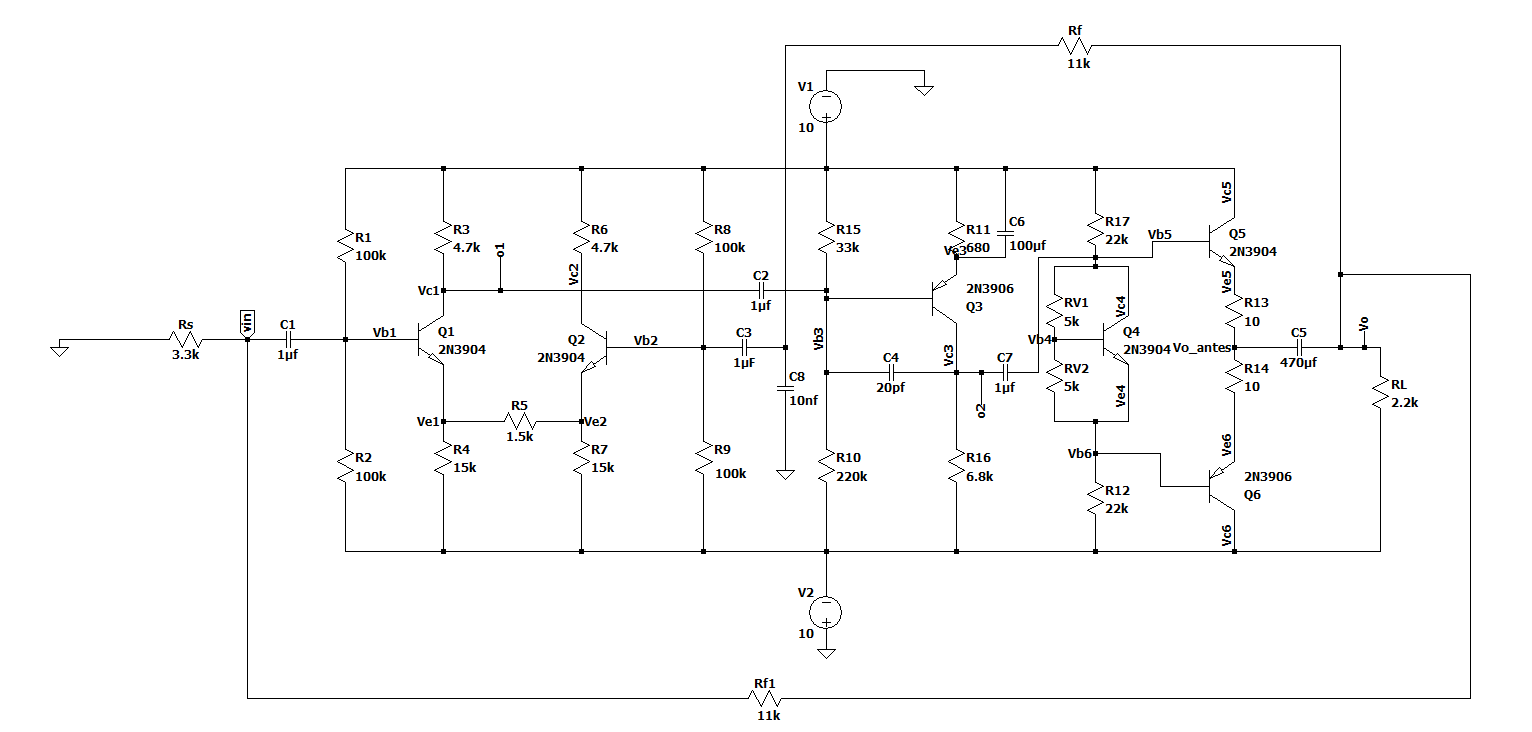
\includegraphics[width=\textwidth]{Imagenes/oscilador.png}
          \caption{Diagrama esquemático del amplificador base realimentado negativamente y positivamente.}
          \label{fig:oscilador}
        \end{figure}
        \subsubsection{Simulación}

  \item \textbf{Realice la simulación del circuito con el fin de verificar los cálculos previos.}
        \begin{itemize}
          \item \textbf{Realimentación negativa}



                \begin{figure}[H]
                  \centering
                  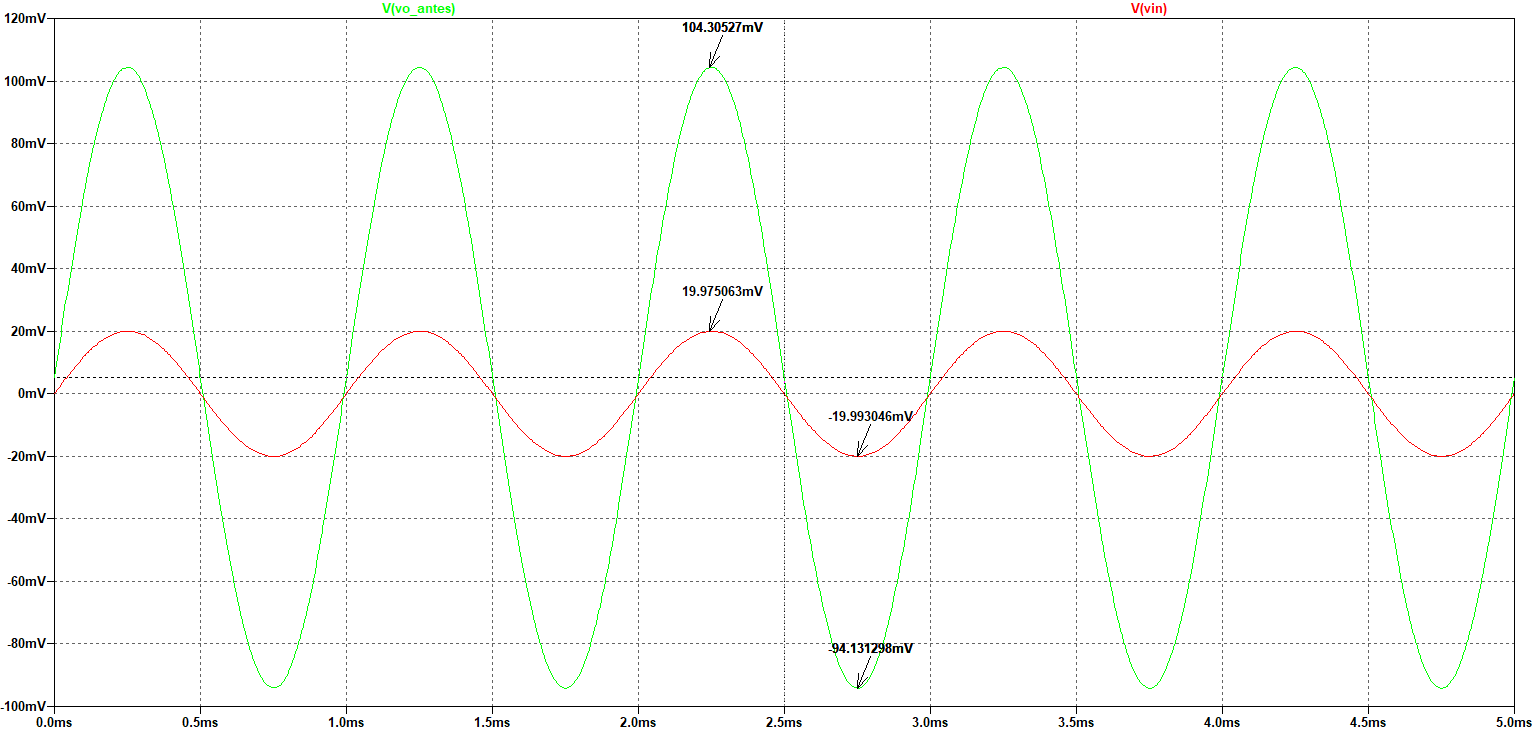
\includegraphics[width=\textwidth]{Imagenes/sim_vovi_realimentadon.png}
                  \captionsetup{labelfont={bf}}
                  \caption{Simulación del circuito de la figura \ref{fig:realimentadon}.}
                  \label{fig:sim_vovi_retroalimentadon}
                \end{figure}

                Si verificamos la ganancia de la realimentación negativa se tiene lo siguiente:

                \begin{align*}
                  A_{fb} & = \dfrac{104.30527m-(-94.131298m)}{19.975063m-(-19.993046m)} \\[0.2cm]
                  A_{fb} & = 4.965                                                      \\[0.2cm]
                \end{align*}

                Los valores son muy cercanos a los teóricos.

                \begin{figure}[H]
                  \centering
                  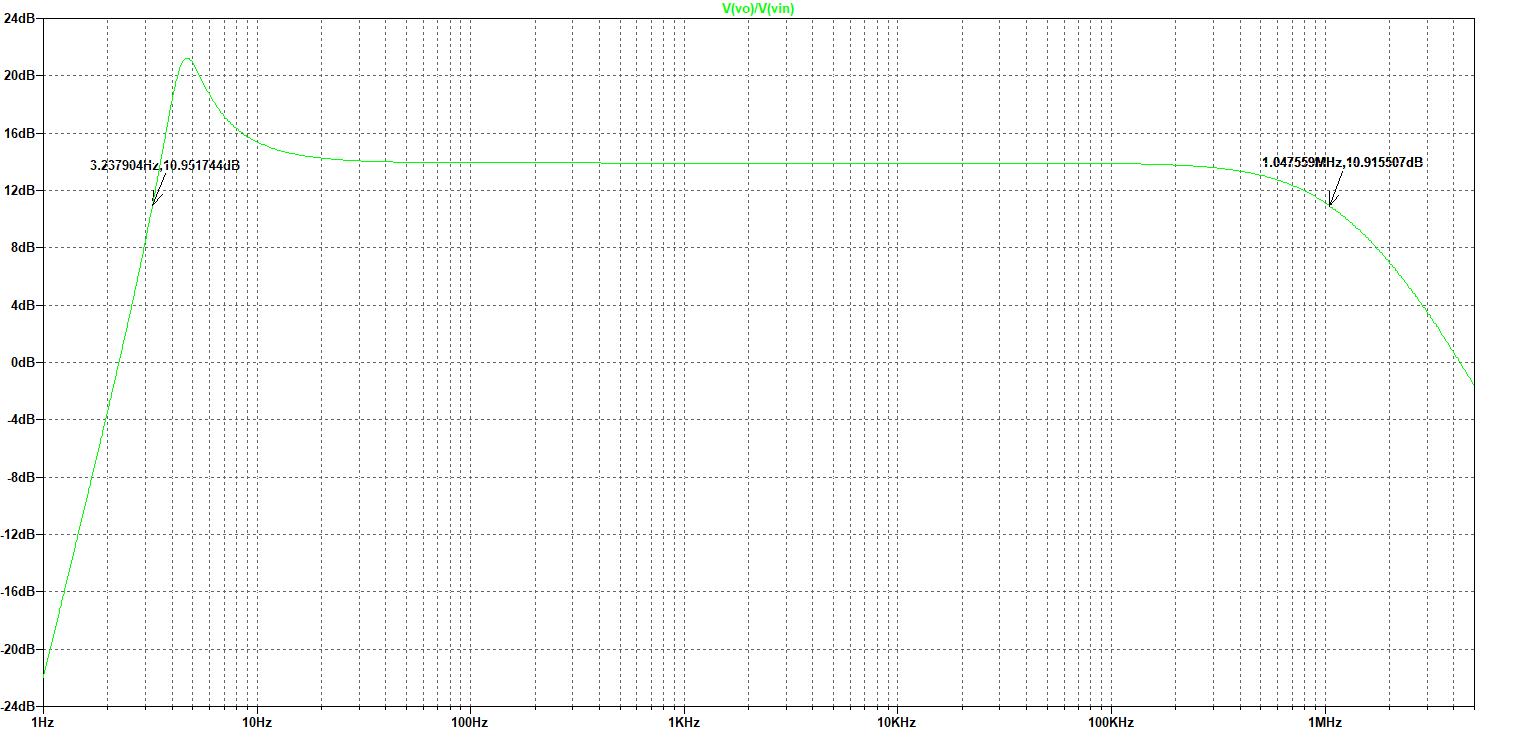
\includegraphics[width=\textwidth]{Imagenes/sim_resp_realimentadon.png}
                  \captionsetup{labelfont={bf}}
                  \caption{Simulación de la respuesta en frecuencia del circuito de la figura \ref{fig:realimentadon} .}
                  \label{fig:sim_resp_retroalimentadon}
                \end{figure}

                Son valores validos para los valores teóricos.

          \item \textbf{Realimentación negativa y positiva (oscilador)}


                \begin{figure}[H]
                  \centering
                  \includegraphics[width=\textwidth]{Imagenes/sim_oscilador.png}
                  \captionsetup{labelfont={bf}}
                  \caption{Simulación del circuito de la figura \ref{fig:oscilador}.}
                  \label{fig:sim_oscilador}
                \end{figure}

                Sin alimentación de entrada se observa sus oscilaciones por las realimentaciones debido a que este se convierte en un amplificador inestable por su realimentación positiva, sin embargo posee varias funcionalidades.
        \end{itemize}
\end{enumerate}








































































\newpage




%Equipos e instrumentos

\section{Equipos e instrumentos}

\begin{table}[H]
    \centering
    \begin{tabular}{|c|c|c|}
        \hline
        \textbf{Equipo} & \textbf{Marca} & \textbf{Modelo} \\\hline
        Osciloscopio Digital & UNI-T & UTD2102CEX+ \\\hline
        Fuente de alimentación & UNI-T & UTP3305-II \\\hline
        Generador de señales & UNI-T & UTG932E \\\hline
        Multímetro Digital & BAKU & 9205A \\\hline
        Multímetro Digital & PROJECTA & DT830D \\\hline
    \end{tabular}    
    \captionsetup{labelfont={bf}}
    \caption{Relación de Equipos e Instrumentos}
    \label{tab:equipos}
\end{table}


%Componentes y materiales

\section{Componentes y materiales}

\begin{table}[H]
    \centering
    \begin{tabular}{|c|c|c|}
        \hline
        \textbf{Componente} & \textbf{Valor} & \textbf{Cantidad} \\\hline
        \textbf{Protoboard} & - & 1 \\\hline
        \textbf{Puntas de osciloscopio} & - & 3 \\\hline
        \textbf{Diodos} & 1N400X ($1\leq x \leq 7$) / 1N4148 & 5 \\\hline
        \multirow{2}{5cm}{\centering \textbf{Circuito Integrado}}
         & LM741 & 5 \\
         & 7805 & 1 \\\hline
        \multirow{2}{5cm}{\centering \textbf{Resistencia variable}}
         & $1 \, k  \si{\ohm}\pm5 \%$ & 1 \\
         & $10 \, k  \si{\ohm}\pm5 \%$ & 1 \\\hline
        \multirow{14}{5cm}{\centering \textbf{Resistencia}}
        & $3.9 \, \si{\ohm}\pm5\%$ & 1 \\
        & $68 \, \si{\ohm}\pm5\%$ & 3 \\
        & $100 \, \si{\ohm}\pm5\%$ & 2 \\
        & $240 \, \si{\ohm}\pm5\%$ & 3 \\
        & $1 \, k  \si{\ohm}\pm5\%$ & 7 \\
        & $2.2 \, k  \si{\ohm}\pm5\%$ & 11 \\
        & $3.3 \, k  \si{\ohm}\pm5\%$ & 2 \\
        & $3.9 \, k  \si{\ohm}\pm5\%$ & 5 \\
        & $5.1 \, k  \si{\ohm}\pm5\%$ & 3 \\
        & $8.2 \, k  \si{\ohm}\pm5\%$ & 1 \\
        & $10 \, k  \si{\ohm}\pm5\%$ & 9 \\
        & $20 \, k  \si{\ohm}\pm5\%$ & 2 \\
        & $100 \, k  \si{\ohm}\pm5\%$ & 2 \\
        & $22 \, M  \si{\ohm}\pm5\%$ & 2 \\\hline
         \multirow{4}{5cm}{\centering \textbf{Condensador}}
        & $10 \,  nF\pm20\%$ & 5 \\
        & $80 \, nF\pm20\%$ & 1 \\
        & $100 \, nF\pm20\%$ & 2 \\
        & $470 \, \mu F\pm20\%$ & 1 \\\hline
        \textbf{Transformador} & 120VAC 60HZ / 12V & 1 \\\hline
    \end{tabular}
    \captionsetup{labelfont={bf}}
    \caption{Relación de Componentes y Materiales (Bill of Materials (BOM))}
    \label{tab:componentes}
\end{table}



\newpage

%Resultados

\section{Resultados}\label{sec:resultados}
\subsection{Parte 1. Amplificador de potencia} \label{subsec:parte1}

\begin{enumerate}
  \item \textbf{Mida los puntos de operación de todos los elementos activos, con el fin de verificar el correcto funcionamiento del circuito.}

        \begin{table}[H]
          \centering
          \begin{tabular}{|c|c|c|c|c|c|c|}
            \hline
            \textbf{Transistor} & \textbf{Vc[V]} & \textbf{$\Delta Vc[V]$} & \textbf{Vb[V]} & \textbf{$\Delta Vb[V]$} & \textbf{Ve[V]} & \textbf{$\Delta Ve[V]$} \\
            \hline
            Q4                  & 300m           & $\pm$ 20m               & 0m             & $\pm$ 20m               & -600m          & $\pm$ 40m               \\
            Q5                  & 10             & $\pm$ 1                 & 600m           & $\pm$ 40m               & 20m            & $\pm$ 4m                \\
            Q6                  & -10            & $\pm$ 1                 & -600m          & $\pm$ 40m               & 20m            & $\pm$ 4m                \\
            \hline
          \end{tabular}
          \caption{mediciones para hallar puntos de operación}
          \label{tab:pto_oper1}
        \end{table}

        Haciendo uso de las ecuaciones \ref{eqn:incertidumbre_vce} y \ref{eqn:incertidumbre_ic}, hallamos sus puntos de operación.

        \begin{itemize}
          \item $\mathbf{V_{CEQ}}$

                \begin{align*}
                  \Delta V_{CEQ_4} & = \sqrt{\left(\Delta V_C\right)^2 + \left(\Delta V_E\right)^2}     \\[0.2cm]
                  \Delta V_{CEQ_4} & = \sqrt{\left(0.04\right)^2 + \left(0.04\right)^2}=\pm 44.72m\volt \\[0.2cm]
                  \Delta V_{CEQ_5} & = \sqrt{\left(1\right)^2 + \left(0.02\right)^2}=\pm 1\volt         \\[0.2cm]
                  \Delta V_{CEQ_6} & = \sqrt{\left(1\right)^2 + \left(0.02\right)^2}=\pm 1\volt         \\[1cm]
                  V_{CEQ_4}        & =0.3-(-0.6)=0.9 \pm 0.04472\volt                                   \\[0.2cm]
                  V_{CEQ_5}        & =10-(0.02)=9.98 \pm 1\volt                                         \\[0.2cm]
                  V_{CEQ_6}        & =-10-(0.02)=-10.02 \pm 1\volt                                      \\[1cm]
                \end{align*}


          \item $\mathbf{I_{CQ}}$

                \begin{align*}
                  \Delta I_{c}   & = \sqrt{\left(\frac{\Delta V_{A}}{R}\right)^2 + \left(\frac{\Delta V_{B}}{R}\right)^2 + \left(\frac{(V_{A} - V_{B}) \cdot \Delta R}{R^2}\right)^2} \\[0.2cm]
                  \Delta I_{c5}  & = \sqrt{\left(\frac{1}{22k}\right)^2 + \left(\frac{0.04}{22k}\right)^2 + \left(\frac{(10-0.6) \cdot 0.05(22k)}{22k^2}\right)^2}                    \\[0.2cm]
                  \Delta I_{c_5} & =\Delta I_{c_6} =\pm 50.257\mu A                                                                                                                   \\[0.2cm]
                  \Delta I_{c_4} & = \sqrt{\left(\frac{1}{27k}\right)^2 + \left(\frac{0.02}{27k}\right)^2 + \left(\frac{(10-(0)) \cdot 0.05(27k)}{27k^2}\right)^2}                    \\[0.2cm]
                  \Delta I_{c_4} & =\pm 47.42\mu A                                                                                                                                    \\[1cm]
                  I_{CQ_4}       & =\dfrac{10-(0)}{27k}=370 \pm 47.42\mu A                                                                                                            \\[0.2cm]
                  I_{CQ_5}       & = I_{CQ_6}=\dfrac{10-(0.6)}{22k}=427.27 \pm 50.257\mu A                                                                                            \\[0.2cm]
                \end{align*}
        \end{itemize}

        \begin{table}[H]
          \centering
          \begin{tabular}{|c|c|c|c|c|c|c|}
            \hline
            \textbf{Transistores} & $v_{CE} [V]$ & $\Delta V_{CE} [V]$  & $E_{r_{V_{CE}}} [\%]$ & $I_{C} [\mu A]$ & $\Delta I_{C} [\mu A]$ & $E_{r_{I_{C}}} [\%]$ \\
            \hline
            $Q_4$                 & $0.9$        & $\pm 44.72 \text{m}$ & $30.77 \text{m}$      & $370$           & $\pm 47.42$            & $25.42$              \\
            \hline
            $Q_5$                 & $9.98$       & $\pm 1$              & $0.2$                 & $427.27$        & $\pm 50.257$           & $7.39$               \\
            \hline
            $Q_6$                 & $-10.02$     & $\pm 1$              & $0.2$                 & $427.27$        & $\pm 50.257$           & $7.39$               \\
            \hline
          \end{tabular}
          \caption{Mediciones indirectas con sus errores relativos de sus puntos de operación }
          \label{tab:puntos_operacion_experimental_maserror}
        \end{table}


  \item \textbf{Con ayuda del generador de funciones, determine el modelo circuital a pequeña señal y a frecuencias medias (1kHz aprox.) de la EP.}

        \begin{table}[H]
          \centering
          \begin{tabular}{|c|c|c|c|c|c|c|}
            \hline
            \textbf{Vi[V\_p]} & $\mathbf{\Delta Vi[V\_p]}$ & \textbf{Vo[V\_p]} & $\mathbf{\Delta Vo[V\_p]}$ & \textbf{A[V/V]} & $\mathbf{\Delta A[V/V]}$ \\
            \hline
            1                 & $\pm$ 0.1                  & 1                 & $\pm$ 0.1                  & 1               & $\pm$ 141.42 m           \\
            \hline
          \end{tabular}
          \caption{Mediciones de ganancia en la etapa de potencia (EP)}
          \label{tab:ganancia_ep}
        \end{table}

        En la tabla \ref{tab:ganancia_ep} se hallo el $\mathbf{\Delta A[V/V]}$ gracias a la ecuación \ref{eqn:incertidumbre_av}

        \begin{table}[H]
          \centering
          \begin{tabular}{|c|c|}
            \hline
            $E_{r_{A_v}} [\%]$ & 2.77 \\
            \hline
          \end{tabular}
          \caption{Error porcentual de la ganancia}
          \label{tab:error_porcentual1_av}
        \end{table}


        \begin{itemize}
          \item \textbf{Impedancia de entrada}
                Acá sacamos las incertidumbres gracias a la ecuación \ref{eqn:incertidumbre}.

                \begin{table}[H]
                  \centering
                  \begin{tabular}{|c|c|c|c|c|c|c|c|}
                    \hline
                    $\mathbf{V_g[V_p]}$ & $\mathbf{\Delta V_g[V_p]}$ & $\mathbf{V_i[V_p]}$ & $\mathbf{\Delta V_i[V_p]}$ & $\mathbf{R_p[\Omega]}$ & $\mathbf{\Delta R_p[\%]}$ & $\mathbf{Z_{in}[\Omega]}$ & $\mathbf{\Delta Z_{in}[\Omega]}$ \\
                    \hline
                    1                   & 0.1                        & 0.5                 & 0.1                        & $11 k +50$             & $1\%$                     & $11k$                     & $\pm 4.92k$                      \\
                    \hline
                  \end{tabular}
                  \caption{Medición de impedancias de entrada}
                  \label{tab:med_zin_ep}
                \end{table}

                \begin{table}[H]
                  \centering
                  \begin{tabular}{|c|c|}
                    \hline
                    $E_{r_{Z_{in}}} [\%]$ & 3.19 \\
                    \hline
                  \end{tabular}
                  \caption{Error porcentual de la impedancia de entrada}
                  \label{tab:error_porcentual1_zin}
                \end{table}

          \item \textbf{Impedancias de salida}

                \begin{table}[H]
                  \centering
                  \begin{tabular}{|c|c|c|c|c|c|c|c|}
                    \hline
                    \textbf{Vo\_sc[V\_p]} & $\mathbf{\Delta vo\_sc[V\_p]}$ & \textbf{Vo\_cc[V\_p]} & $\mathbf{\Delta Vo\_cc[V\_p]}$ & \textbf{Rp[$\Omega$]} & $\mathbf{\Delta Rp[\Omega]}$ & \textbf{Zo[$\Omega$]} & $\mathbf{\Delta Zo[\Omega]}$ \\
                    \hline
                    1                     & 0.1                            & 0.9                   & 0.1                            & 180                   & 5\%                          & 20                    & $\pm$ 29.91                  \\
                    \hline
                  \end{tabular}
                  \caption{Medición de impedancia de salida}
                  \label{tab:med_zo_ep}
                \end{table}
        \end{itemize}

        \begin{table}[H]
          \centering
          \begin{tabular}{|c|c|}
            \hline
            $E_{r_{Z_{o}}} [\%]$ & 73.18 \\
            \hline
          \end{tabular}
          \caption{Error porcentual de la impedancia de salida}
          \label{tab:error_porcentual1_zo}
        \end{table}


  \item \textbf{Modificando la polarización de la etapa, conviértala en:}
        \begin{enumerate}
          \item \textbf{Un amplificador clase B, colocando los transistores
                  de potencia justo en la zona de corte.}

                En la siguiente imagen se muestra el efecto de cruce, debido a la manipulación de la resistencia variable o potenciómetro.

                \begin{figure}[H]
                  \centering
                  \renewcommand{\figurename}{Imagen}
                  \setcounter{figure}{0}
                  \includegraphics[width=\textwidth]{Imagenes/crossover_b.jpg}
                  \caption{Efecto crossover en un amplificador Tipo B. Siendo X=0.56}
                  \label{fig:crossover_b}
                \end{figure}

                \begin{table}[H]
                  \centering
                  \begin{tabular}{|c|c|c|c|}
                    \hline
                    \textbf{time/div} $[\mu s]$ & \textbf{Channel} & \textbf{voltios/div $[\volt]$} & \textbf{Acoplamiento} \\ \hline
                    $200 \, \pm 40 \,  $        & 1 (Azul)         & $500 \pm 100 \text{m}  $       & AC                    \\ \hline
                    $200 \, \pm 40 \,  $        & 2 (Amarillo)     & $500 \pm 100 \text{m}   $      & AC                    \\ \hline
                  \end{tabular}
                  \caption{Escalas Usada en el Osciloscopio Digital UNI-T UTD2102CEX+}
                  \label{tab:escala_crossover_b}
                \end{table}


          \item \textbf{Un amplificador clase AB, colocando los transistores de potencia conduciendo con corriente pequeñas.}

                \begin{figure}[H]
                  \centering
                  \renewcommand{\figurename}{Imagen}
                  \includegraphics[width=\textwidth]{Imagenes/sincrossover.jpg}
                  \caption{Sin Efecto crossover Se convierte en un amplificador Tipo AB. Siendo X=0.5}
                  \label{fig:sincrossover}
                \end{figure}


                \begin{table}[H]
                  \centering
                  \begin{tabular}{|c|c|c|c|}
                    \hline
                    \textbf{time/div} $[\mu s]$ & \textbf{Channel} & \textbf{voltios/div $[\volt]$} & \textbf{Acoplamiento} \\ \hline
                    $200 \, \pm 40 \, $         & 1 (Azul)         & $500 \pm 100 \text{m}  $       & AC                    \\ \hline
                    $200 \, \pm 40 \,   $       & 2 (Amarillo)     & $500  \pm 100 \text{m}   $     & AC                    \\ \hline
                  \end{tabular}
                  \caption{Escalas Usada en el Osciloscopio Digital UNI-T UTD2102CEX+}
                  \label{tab:escala_sincrossover}
                \end{table}
        \end{enumerate}
\end{enumerate}

\subsection{Parte 2. Amplificador Diferencial} \label{subsec:parte2}

\begin{enumerate}
  \item \textbf{Mida los puntos de operación de todos los elementos activos, con el fin de verificar el correcto funcionamiento del circuito.}

        \begin{table}[H]
          \centering
          \begin{tabular}{|c|c|c|c|c|c|c|}
            \hline
            \textbf{Transistor} & $\mathbf{Vc[V]}$ & $\mathbf{\Delta Vc[V]}$ & $\mathbf{Vb[V]}$ & $\mathbf{\Delta Vb[V]}$ & $\mathbf{Ve[V]}$ & $\mathbf{\Delta Ve[V]}$ \\
            \hline
            Q1                  & 8                & $\pm$ 1                 & -120m            & $\pm$ 20m               & -700m            & $\pm$ 100m              \\
            \hline
            Q2                  & 7.2              & $\pm$ 0.4               & -60m             & $\pm$ 10m               & -680m            & $\pm$ 40m               \\
            \hline
          \end{tabular}
          \caption{Mediciones para hallar punto de operación}
          \label{tab:pto_ope_ed}
        \end{table}
        Haciendo uso de las ecuaciones \ref{eqn:incertidumbre_vce} y \ref{eqn:incertidumbre_ic}, hallamos sus puntos de operación e incertidumbres.

        \begin{itemize}
          \item $\mathbf{V_{CEQ}}$

                \begin{align*}
                  \Delta V_{CEQ_1} & = \sqrt{\left(\Delta V_C\right)^2 + \left(\Delta V_E\right)^2}   \\[0.2cm]
                  \Delta V_{CEQ_1} & = \sqrt{\left(1\right)^2 + \left(0.1\right)^2}=\pm 1.005 \volt   \\[0.2cm]
                  \Delta V_{CEQ_2} & = \sqrt{\left(0.4\right)^2 + \left(0.04\right)^2}=\pm 0.402\volt \\[1cm]
                  V_{CEQ_1}        & =8-(-0.7)=8.7 \pm 1.005\volt                                     \\[0.2cm]
                  V_{CEQ_2}        & =7.2-(-0.68)=7.88 \pm 0.402\volt                                 \\[1cm]
                \end{align*}


          \item $\mathbf{I_{CQ}}$

                \begin{align*}
                  \Delta I_{c}   & = \sqrt{\left(\frac{\Delta V_{A}}{R}\right)^2 + \left(\frac{\Delta V_{B}}{R}\right)^2 + \left(\frac{(V_{A} - V_{B}) \cdot \Delta R}{R^2}\right)^2} \\[0.2cm]
                  \Delta I_{c1}  & = \sqrt{\left(\frac{1}{4.7k}\right)^2 + \left(\frac{1}{4.7k}\right)^2 + \left(\frac{(10-8) \cdot 0.05(4.7k)}{4.7k^2}\right)^2}                     \\[0.2cm]
                  \Delta I_{c_1} & =\pm 301.648\mu A                                                                                                                                  \\[1cm]
                  \Delta I_{c2}  & = \sqrt{\left(\frac{1}{4.7k}\right)^2 + \left(\frac{0.4}{4.7k}\right)^2 + \left(\frac{(10-7.2) \cdot 0.05(4.7k)}{4.7k^2}\right)^2}                 \\[0.2cm]
                  \Delta I_{c_2} & =\pm 231.084 \mu A                                                                                                                                 \\[1cm]
                  I_{CQ_1}       & =\dfrac{10-(8)}{4.7k}=425.532 \pm 301.648\mu A                                                                                                     \\[1cm]
                  I_{CQ_2}       & =\dfrac{10-(7.2)}{4.7k}=595.745 \pm 231.084\mu A                                                                                                   \\[1cm]
                \end{align*}

        \end{itemize}

        \begin{table}[H]
          \centering
          \begin{tabular}{|c|c|c|c|c|c|c|}
            \hline
            \textbf{Transistores} & $v_{CE} [V]$ & $\Delta V_{CE} [V]$ & $E_{r_{V_{CE}}} [\%]$ & $I_{C} [\mu A]$ & $\Delta I_{C} [\mu A]$ & $E_{r_{I_{C}}} [\%]$ \\
            \hline
            $Q_1$                 & $8.7$        & $\pm 1.005 $        & $8.75$                & $425.532$       & $\pm 301.648$          & $29.76$              \\
            \hline
            $Q_2$                 & $7.88$       & $\pm 0.402$         & $1.5$                 & $595.745$       & $\pm 231.084$          & $1.66$               \\
            \hline
          \end{tabular}
          \caption{Mediciones indirectas con sus errores relativos de sus puntos de operación }
          \label{tab:puntos_operacion_experimental_maserror_parte2}
        \end{table}

  \item \textbf{Con la metodología expuesta por Ud. en el trabajo de preparación, determine el modelo completo del amplificador diferencial.}
        \begin{table}[H]
          \centering
          \begin{tabular}{|c|c|c|c|c|c|}
            \hline
            \textbf{Vi[V\textsubscript{p}]} & \textbf{\(\Delta\)Vi[V\textsubscript{p}]} & \textbf{Vo[V\textsubscript{p}]} & \textbf{\(\Delta\)Vo[V\textsubscript{p}]} & \textbf{$A_d$[V/V]} & \textbf{\(\Delta\)$A_d$[V/V]} \\\hline
            1                               & \(\pm\) 0.2                               & 3                               & \(\pm\) 0.2                               & 3                   & \(\pm\) 632.46m               \\\hline
          \end{tabular}
          \caption{Mediciones de ganancia en modo diferencial de la Etapa diferencial (ED)}
          \label{tab:ganancia_ed}
        \end{table}

        \begin{table}[H]
          \centering
          \begin{tabular}{|c|c|}
            \hline
            $E_{r_{A_d}} [\%]$ & 1.70 \\
            \hline
          \end{tabular}
          \caption{Error porcentual de la ganancia en modo diferencial}
          \label{tab:error_porcentual2_ad}
        \end{table}

        \begin{table}[H]
          \centering
          \begin{tabular}{|c|c|c|c|c|c|}
            \hline
            \textbf{Vi[V\textsubscript{p}]} & \textbf{\(\Delta\)Vi[V\textsubscript{p}]} & \textbf{Vo[V\textsubscript{p}]} & \textbf{\(\Delta\)Vo[V\textsubscript{p}]} & \textbf{$A_c$ [V/V]} & \textbf{\(\Delta\)$A_c$[V/V]} \\\hline
            1                               & \(\pm\) 0.2                               & 300m                            & \(\pm\) 20m                               & 0.3                  & \(\pm\) 208.81m               \\\hline
          \end{tabular}
          \caption{Mediciones de ganancia en modo común de la Etapa diferencial (ED)}
          \label{tab:ganancia_ed_modo_comun}
        \end{table}


        \begin{table}[H]
          \centering
          \begin{tabular}{|c|c|}
            \hline
            $E_{r_{A_c}} [\%]$ & 3.23 \\
            \hline
          \end{tabular}
          \caption{Error porcentual de la ganancia en modo común}
          \label{tab:error_porcentual2_ac}
        \end{table}

        \begin{table}[H]
          \centering
          \begin{tabular}{|c|c|c|}
            \hline
            CMRR $(\rho) [dB]$ & $\Delta$ CMRR $(\rho) [dB]$ & $E_{r_{\rho}} [\%]$ \\
            \hline
            20                 & $\pm 14.55$                 & $2.20$              \\
            \hline
          \end{tabular}
          \caption{Medida indirecta del CMRR de la ED}
          \label{tab:medida_indirecta_cmrr_ed}
        \end{table}


        \begin{table}[H]
          \centering
          \begin{tabular}{|c|c|c|c|c|c|c|c|}
            \hline
            \textbf{Vg[V\textsubscript{p}]} & \textbf{\(\Delta\)Vg[V\textsubscript{p}]} & \textbf{Vi[V\textsubscript{p}]} & \textbf{\(\Delta\)Vi[V\textsubscript{p}]} & \textbf{Rp[Ω]} & \textbf{\(\Delta\)Rp[Ω]} & \textbf{Zd[Ω]} & \textbf{\(\Delta\)Zd[Ω]} \\\hline
            1                               & \(\pm\) 0.2                               & 0.44                            & \(\pm\) 0.04                              & 39k            & \(\pm\) 5\%              & 30.64k         & \(\pm\) 12.119k          \\\hline
          \end{tabular}
          \caption{Medición de impedancia de entrada en modo diferencial}
          \label{tab:impedancia_entrada_diferencial}
        \end{table}


        \begin{table}[H]
          \centering
          \begin{tabular}{|c|c|}
            \hline
            $E_{r_{Z_{d}}} [\%]$ & 25.92 \\
            \hline
          \end{tabular}
          \caption{Error porcentual de la impedancia de entrada en modo diferencial}
          \label{tab:error_porcentual2_zd}
        \end{table}


        \begin{table}[H]
          \centering
          \begin{tabular}{|c|c|c|c|c|c|c|c|}
            \hline
            \textbf{Vg[V\textsubscript{p}]} & \textbf{\(\Delta\)Vg[V\textsubscript{p}]} & \textbf{Vi[V\textsubscript{p}]} & \textbf{\(\Delta\)Vi[V\textsubscript{p}]} & \textbf{Rp[Ω]} & \textbf{\(\Delta\)Rp[Ω]} & \textbf{Zc[Ω]} & \textbf{\(\Delta\)Zc[Ω]} \\\hline
            1                               & \(\pm\) 0.2                               & 0.32                            & \(\pm\) 0.02                              & 47k            & \(\pm\) 5\%              & 44.24k         & \(\pm\) 13.809k          \\\hline
          \end{tabular}
          \caption{Medición de impedancias de entrada en modo común}
          \label{tab:impedancias_entrada_comun}
        \end{table}

        \begin{table}[H]
          \centering
          \begin{tabular}{|c|c|}
            \hline
            $E_{r_{Z_{c}}} [\%]$ & 9.44 \\
            \hline
          \end{tabular}
          \caption{Error porcentual de la impedancia de entrada en modo común}
          \label{tab:error_porcentual2_zc}
        \end{table}


        \begin{table}[H]
          \centering
          \begin{tabular}{|c|c|c|c|c|c|c|c|}
            \hline
            \textbf{Vo\_sc[V\textsubscript{p}]} & \textbf{\(\Delta\)vo\_sc[V\textsubscript{p}]} & \textbf{Vo\_cc[V\textsubscript{p}]} & \textbf{\(\Delta\)Vo\_cc[V\textsubscript{p}]} & \textbf{Rp[Ω]} & \textbf{\(\Delta\)Rp[Ω]} & \textbf{Zo[Ω]} & \textbf{\(\Delta\)Zo[Ω]} \\\hline
            3                                   & \(\pm\) 0.2                                   & 1.4                                 & \(\pm\) 0.1                                   & 4.7k           & \(\pm\) 5\%              & 5.37k          & \(\pm\) 1.02k            \\\hline
          \end{tabular}
          \caption{Medición de impedancia de salida}
          \label{tab:impedancias_salida}
        \end{table}


        \begin{table}[H]
          \centering
          \begin{tabular}{|c|c|}
            \hline
            $E_{r_{Z_{o}}} [\%]$ & 14.26 \\
            \hline
          \end{tabular}
          \caption{Error porcentual de la impedancia de salida}
          \label{tab:error_porcentual2_zo}
        \end{table}


  \item \textbf{Determine los limites de excursión: en modo diferencial
          y en modo común. en cada caso dibuje o fotografié las señales de salida (ambas salidas asimétricas) en máxima excursión.}

        \begin{figure}[H]
          \centering
          \renewcommand{\figurename}{Imagen}
          \includegraphics[width=\textwidth]{Imagenes/vod.png}
          \caption{Limite de excursión en modo diferencial.}
          \label{fig:vod}
        \end{figure}

        \begin{table}[H]
          \centering
          \begin{tabular}{|c|c|c|c|}
            \hline
            \textbf{time/div} $[\mu s]$ & \textbf{Channel} & \textbf{voltios/div $[\volt]$} & \textbf{Acoplamiento} \\ \hline
            $200 \, \pm 40 \, $         & 1 (Azul)         & $1 \pm 0.2  $                  & AC                    \\ \hline
          \end{tabular}
          \caption{Escalas Usada en el Osciloscopio Digital UNI-T UTD2102CEX+}
          \label{tab:escala_lim_mododif}
        \end{table}

        \begin{table}[H]
          \centering
          \begin{tabular}{|c|c|}
            \hline
            $\mathbf{V_i > 2.2 V_p}$ & $\mathbf{-3.9V_p <V_o<3.9V_p}$ \\
            \hline
          \end{tabular}
          \caption{Limites de excursión de la etapa diferencial en modo diferencial}
          \label{tab:exp_lim_exc_modif}
        \end{table}



        \begin{figure}[H]
          \centering
          \renewcommand{\figurename}{Imagen}
          \includegraphics[width=\textwidth]{Imagenes/voc.png}
          \caption{Limite de excursión en modo común.}
          \label{fig:voc}
        \end{figure}


        \begin{table}[H]
          \centering
          \begin{tabular}{|c|c|c|c|}
            \hline
            \textbf{time/div} $[\mu s]$ & \textbf{Channel} & \textbf{voltios/div $[\volt]$} & \textbf{Acoplamiento} \\ \hline
            $200 \, \pm 40 \, $         & 1 (Azul)         & $1 \pm 0.2  $                  & AC                    \\ \hline
          \end{tabular}
          \caption{Escalas Usada en el Osciloscopio Digital UNI-T UTD2102CEX+}
          \label{tab:escala_lim_modocomun}
        \end{table}

        \begin{table}[H]
          \centering
          \begin{tabular}{|c|c|}
            \hline
            $\mathbf{V_i > 12 V_p}$ & $\mathbf{-2.4V_p <V_o<2.4V_p}$ \\
            \hline
          \end{tabular}
          \caption{Límites de excursión de la etapa diferencial en modo común}
          \label{tab:exp_lim_exc_mocom}
        \end{table}

\end{enumerate}

\subsection{Parte 3. Amplificador multietapas} \label{subsec:parte3}

\begin{enumerate}

  \item \textbf{Determine experimentalmente para cada etapa desacoplada,
          los puntos de operación de los elementos activos y los modelos dinámicos de cada etapa.}

        \begin{table}[H]
          \centering
          \begin{tabular}{|c|c|c|c|c|c|c|}
            \hline
            \textbf{Transistor} & \textbf{Vc[V]} & $\mathbf{\Delta Vc[V]}$ & \textbf{Vb[V]} & $\mathbf{\Delta Vb[V]}$ & \textbf{Ve[V]} & $\mathbf{\Delta Ve[V]}$ \\ \hline
            Q1                  & 7.2            & $\pm 0.4$               & 240m           & $\pm 20m$               & -360m          & $\pm 100m$              \\ \hline
            Q2                  & 7.2            & $\pm 0.4$               & 260m           & $\pm 20m$               & -360m          & $\pm 20m$               \\ \hline
            Q3                  & 5.2            & $\pm 0.4$               & 8              & $\pm 0.4$               & 9              & $\pm 1$                 \\ \hline
            Q4                  & 900m           & $\pm 100m$              & 360m           & $\pm 20m$               & -200m          & $\pm 20m$               \\ \hline
            Q5                  & 10             & $\pm 1$                 & 900m           & $\pm 100m$              & 380m           & $\pm 20m$               \\ \hline
            Q6                  & -10            & $\pm 1$                 & -220m          & $\pm 20m$               & 360m           & $\pm 20m$               \\ \hline
          \end{tabular}
          \caption{Mediciones para hallar punto de operación, acoplando sus etapas}
          \label{tab:punto_operacion_aco}
        \end{table}



        Haciendo uso de las ecuaciones \ref{eqn:incertidumbre_vce} y \ref{eqn:incertidumbre_ic}, hallamos sus puntos de operación e incertidumbres (Acoplado).

        \begin{itemize}
          \item $\mathbf{V_{CEQ}}$

                \begin{align*}
                  V_{CEQ_3} & =5.2-(9)=-3.8 \pm 1.08\volt    \\[0.2cm]
                  V_{CEQ_1} & =7.2-(0.36)=7.56 \pm 0.41\volt \\[0.2cm]
                  V_{CEQ_2} & =7.2-(0.36)=7.56 \pm 0.41\volt \\[0.2cm]
                  V_{CEQ_4} & =0.9-(-0.2)=1.1 \pm 0.10\volt  \\[0.2cm]
                  V_{CEQ_5} & =10-(0.38)=9.62 \pm 1\volt     \\[0.2cm]
                  V_{CEQ_6} & =-10-(0.36)=-10.36 \pm 1\volt  \\[1cm]
                \end{align*}


          \item $\mathbf{I_{CQ}}$

                \begin{align*}
                  I_{CQ_3} & =\dfrac{9-(-10)}{6.8k}=2.79 \pm 0.25 mA                   \\[0.2cm]
                  I_{CQ_4} & =\dfrac{10-(-0.36)}{5k}=357.04 \pm 47.12\mu A             \\[0.2cm]
                  I_{CQ_5} & =\dfrac{10-(0.9)}{22k}=413.64 \pm 50.14\mu A              \\[0.2cm]
                  I_{CQ_6} & =\dfrac{-0.22-(-10)}{22k}=444.55 \pm 50.61\mu A           \\[0.2cm]
                  I_{CQ_1} & = I_{CQ_2}=\dfrac{10-(7.2)}{4.7k}=595.74 \pm 231.08 \mu A \\[1cm]
                \end{align*}



                \begin{table}[H]
                  \centering
                  \begin{tabular}{|c|c|c|c|c|c|c|}
                    \hline
                    \textbf{Transistores} & $v_{CE} [V]$ & $\Delta V_{CE} [V]$ & $E_{r_{V_{CE}}} [\%]$ & $I_{C} [\mu A]$ & $\Delta I_{C} [\mu A]$ & $E_{r_{I_{C}}} [\%]$ \\
                    \hline
                    $Q_1$                 & $7.56$       & $\pm 0.41 $         & $5.5$                 & $595.74$        & $\pm 231.08$           & $1.67$               \\
                    \hline
                    $Q_2$                 & $7.56$       & $\pm 0.40 $         & $5.5$                 & $595.74$        & $\pm 231.08$           & $1.67$               \\
                    \hline
                    $Q_3$                 & $-3.8$       & $\pm 1.08$          & $17.48$               & $2790$          & $\pm 250$              & $24.55$              \\
                    \hline
                    $Q_4$                 & $1.1$        & $\pm 0.10$          & $15.38$               & $357.04$        & $\pm 47.12$            & $21.03$              \\
                    \hline
                    $Q_5$                 & $9.62$       & $\pm 1.00$          & $3.8$                 & $413.64$        & $\pm 50.14$            & $3.96$               \\
                    \hline
                    $Q_6$                 & $-10.36$     & $\pm 1.00$          & $3.6$                 & $444.55$        & $\pm 50.61$            & $11.73$              \\
                    \hline
                  \end{tabular}
                  \caption{Mediciones indirectas con sus errores relativos de sus puntos de operación Acoplados}
                  \label{tab:puntos_operacion_experimental_maserror_parte3}
                \end{table}

                \begin{table}[H]
                  \centering
                  \begin{tabular}{|c|c|c|c|c|c|c|}
                    \hline
                    \textbf{Transistor} & \textbf{Vc[V]} & $\mathbf{\Delta Vc[V]}$ & \textbf{Vb[V]} & $\mathbf{\Delta Vb[V]}$ & \textbf{Ve[V]} & $\mathbf{\Delta Ve[V]}$ \\ \hline
                    Q1                  & 7.2            & $\pm 0.4$               & 240m           & $\pm 20m$               & -400m          & $\pm 100m$              \\ \hline
                    Q2                  & 7.2            & $\pm 0.4$               & 240m           & $\pm 20m$               & -360m          & $\pm 20m$               \\ \hline
                    Q3                  & 5.2            & $\pm 0.4$               & 8              & $\pm 0.4$               & 9              & $\pm 1$                 \\ \hline
                    Q4                  & 900m           & $\pm 100m$              & 360m           & $\pm 20m$               & -300m          & $\pm 100m$              \\ \hline
                    Q5                  & 10             & $\pm 1$                 & 900m           & $\pm 100m$              & 360m           & $\pm 20m$               \\ \hline
                    Q6                  & -10            & $\pm 1$                 & -240m          & $\pm 20m$               & 360m           & $\pm 20m$               \\ \hline
                  \end{tabular}
                  \caption{Mediciones para hallar punto de operación, desacoplando sus etapas, colocando un jumper en C2, C5, y C7}
                  \label{tab:punto_operacion_desaco}
                \end{table}




                Haciendo uso de las ecuaciones \ref{eqn:incertidumbre_vce} y \ref{eqn:incertidumbre_ic}, hallamos sus puntos de operación e incertidumbres (Desacoplado).

                En este caso, solo varia en desacople $V_{b_6}$, $V_{e_1}$, $V_{e_4}$ y $V_{e_5}$, sabiendo eso, solo se modificaran dichos valores que sean afectados por estos parámetros.
          \item $\mathbf{V_{CEQ}}$

                \begin{align*}
                  V_{CEQ_3} & =5.2-(9)=-3.8 \pm 1.08\volt    \\[0.2cm]
                  V_{CEQ_1} & =7.2-(-0.4)=7.6 \pm 0.41\volt  \\[0.2cm]
                  V_{CEQ_2} & =7.2-(0.36)=7.56 \pm 0.41\volt \\[0.2cm]
                  V_{CEQ_4} & =0.9-(-0.3)=1.2 \pm 0.14\volt  \\[0.2cm]
                  V_{CEQ_5} & =10-(0.36)=9.64 \pm 1\volt     \\[0.2cm]
                  V_{CEQ_6} & =-10-(0.36)=-10.36 \pm 1\volt  \\[1cm]
                \end{align*}


          \item $\mathbf{I_{CQ}}$

                \begin{align*}
                  I_{CQ_3} & =\dfrac{9-(-10)}{6.8k}=2.79 \pm 0.25 mA                   \\[0.2cm]
                  I_{CQ_4} & =\dfrac{10-(-0.36)}{5k}=357.04 \pm 47.12\mu A             \\[0.2cm]
                  I_{CQ_5} & =\dfrac{10-(0.9)}{22k}=413.64 \pm 50.14\mu A              \\[0.2cm]
                  I_{CQ_6} & =\dfrac{-0.24-(-10)}{22k}=443.64 \pm 50.61\mu A           \\[0.2cm]
                  I_{CQ_1} & = I_{CQ_2}=\dfrac{10-(7.2)}{4.7k}=595.74 \pm 231.08 \mu A \\[1cm]
                \end{align*}



                \begin{table}[H]
                  \centering
                  \begin{tabular}{|c|c|c|c|c|c|c|}
                    \hline
                    \textbf{Transistores} & $v_{CE} [V]$ & $\Delta V_{CE} [V]$ & $E_{r_{V_{CE}}} [\%]$ & $I_{C} [\mu A]$ & $\Delta I_{C} [\mu A]$ & $E_{r_{I_{C}}} [\%]$ \\
                    \hline
                    $Q_1$                 & $7.6$        & $\pm 0.41 $         & $5$                   & $595.74$        & $\pm 231.08$           & $1.67$               \\
                    \hline
                    $Q_2$                 & $7.56$       & $\pm 0.40 $         & $5.5$                 & $595.74$        & $\pm 231.08$           & $1.67$               \\
                    \hline
                    $Q_3$                 & $-3.8$       & $\pm 1.08$          & $17.48$               & $2790$          & $\pm 250$              & $24.55$              \\
                    \hline
                    $Q_4$                 & $1.2$        & $\pm 0.14$          & $7.69$                & $357.04$        & $\pm 47.12$            & $21.03$              \\
                    \hline
                    $Q_5$                 & $9.64$       & $\pm 1.00$          & $3.6$                 & $413.64$        & $\pm 50.14$            & $3.96$               \\
                    \hline
                    $Q_6$                 & $-10.36$     & $\pm 1.00$          & $3.6$                 & $443.64$        & $\pm 50.61$            & $11.50$              \\
                    \hline
                  \end{tabular}
                  \caption{Mediciones indirectas con sus errores relativos de sus puntos de operación Desacoplados}
                  \label{tab:puntos_operacion_experimental_maserror_parte3_des}
                \end{table}
        \end{itemize}

        \begin{table}[H]
          \centering
          \begin{tabular}{|c|c|c|c|c|c|c|}
            \hline
            \textbf{Vi[V]} & $\mathbf{\Delta Vi[V]}$ & \textbf{Vo[V]} & $\mathbf{\Delta Vo[V]}$ & \textbf{Ad[V/V]} & $\mathbf{\Delta Ad[V/V]}$ \\ \hline
            5m             & $\pm 10m$               & 1              & $\pm 100m$              & 200              & $\pm 20.01$               \\ \hline
            35m            & $\pm 4m$                & 3              & $\pm 0.4m$              & 85.71            & $\pm 11.43$               \\ \hline
            50m            & $\pm 10m$               & 5.2            & $\pm 0.2$               & 104              & $\pm 4.13$                \\ \hline
          \end{tabular}
          \caption{Mediciones de ganancia en modo diferencial en el multietapas}
          \label{tab:ganancia_multietapas}
        \end{table}

        \begin{table}[H]
          \centering
          \begin{tabular}{|c|c|c|}
            \hline
            $A_{d_{teo}} [V/V]$ & $A_{d_{Exp}} [V/V]$ & $E_{r_{A_d}} [\%]$ \\
            \hline
            265,659             & 200                 & 24.72              \\
            \hline
            265,659             & 85.71               & 67.74              \\
            \hline
            265,659             & 104                 & 60.85              \\
            \hline
          \end{tabular}
          \caption{Error porcentual de la ganancia en modo diferencial}
          \label{tab:error_porcentual_ganancia_diferencial}
        \end{table}



        \begin{table}[H]
          \centering
          \begin{tabular}{|c|c|c|c|c|c|c|}
            \hline
            \textbf{Vi[V]} & $\mathbf{\Delta Vi[V]}$ & \textbf{Vo[V]} & $\mathbf{\Delta Vo[V]}$ & \textbf{$A_c[V/V]$} & $\mathbf{\Delta A_c[V/V]}$ \\ \hline
            5m             & $\pm 10m$               & 50m            & $\pm 10m$               & 10                  & $\pm 2.00$                 \\ \hline
            35m            & $\pm 4m$                & 360m           & $\pm 20m$               & 10.29               & $\pm 1.31$                 \\ \hline
            50m            & $\pm 10m$               & 1              & $\pm 100 m$             & 20                  & $\pm 2.00$                 \\ \hline
          \end{tabular}
          \caption{Mediciones de ganancia en modo común en el multietapas}
          \label{tab:ganancia_modocomun_multietapas}
        \end{table}

        \begin{table}[H]
          \centering
          \begin{tabular}{|c|c|c|}
            \hline
            $A_{c_{teo}} [V/V]$ & $A_{c_{Exp}} [V/V]$ & $E_{r_{A_c}} [\%]$ \\
            \hline
            27.91               & 10                  & 64.17              \\
            \hline0
            27.91               & 10.29               & 63.13              \\
            \hline
            27.91               & 20                  & 28.34              \\
            \hline
          \end{tabular}
          \caption{Error porcentual de la ganancia en modo común}
          \label{tab:error_porcentual_ganancia_comun}
        \end{table}

        \begin{table}[H]
          \centering
          \begin{tabular}{|c|c|c|}
            \hline
            CMRR $(\rho) [dB]$ & $\Delta$ CMRR $(\rho) [dB]$ & $E_{r_{\rho}} [\%]$ \\
            \hline
            26.02              & $\pm 4.47$                  & $14.88$             \\
            \hline
          \end{tabular}
          \caption{Medida indirecta del CMRR del multietapas}
          \label{tab:medida_indirecta_cmrr_me}
        \end{table}

        \begin{table}[H]
          \centering
          \begin{tabular}{|c|c|c|c|c|c|c|c|}
            \hline
            \textbf{Vg[V]} & $\mathbf{\Delta Vg[V]}$ & \textbf{Vi[V]} & $\mathbf{\Delta Vi[V]}$ & \textbf{Rp[Ω]} & $\mathbf{\Delta Rp[\ohm]}$ & \textbf{Zd[Ω]} & $\mathbf{\Delta Zd[\ohm]}$ \\ \hline
            12m            & $\pm 1m$                & 7m             & $\pm 1m$                & 47k            & $\pm 5\%$                  & 65.8k          & $\pm 26.32k$               \\ \hline
          \end{tabular}
          \caption{Medición de impedancia de entrada en modo diferencial en el multietapas}
          \label{tab:impedancia_diferencial_multietapas}
        \end{table}

        \begin{table}[H]
          \centering
          \begin{tabular}{|c|c|}
            \hline
            $E_{r_{Z_{d}}} [\%]$ & 59.09 \\
            \hline
          \end{tabular}
          \caption{Error porcentual de la impedancia de entrada modo diferencial}
          \label{tab:error_porcentual3_zid}
        \end{table}


        \begin{table}[H]
          \centering
          \begin{tabular}{|c|c|c|c|c|c|c|c|}
            \hline
            \textbf{Vg[V]} & $\mathbf{\Delta Vg[V]}$ & \textbf{Vi[V]} & $\mathbf{\Delta Vi[V]}$ & \textbf{Rp[}\si{\ohm}\textbf{]} & $\mathbf{\Delta Rp[}\si{\ohm}\textbf{]}$ & \textbf{Zc[}\si{\ohm}\textbf{]} & $\mathbf{\Delta Zc[}\si{\ohm}\textbf{]}$ \\ \hline
            13m            & $\pm 1m$                & 5m             & $\pm 1m$                & 47k                             & $\pm 5\%$                                & 58.75k                          & $\pm 20.67k$                             \\ \hline
          \end{tabular}
          \caption{Medición de impedancias de entrada en modo común en el multietapas}
          \label{tab:impedancias_comun_multietapas}
        \end{table}

        \begin{table}[H]
          \centering
          \begin{tabular}{|c|c|}
            \hline
            $E_{r_{Z_{c}}} [\%]$ & 3.19 \\
            \hline
          \end{tabular}
          \caption{Error porcentual de la impedancia de entrada en modo común}
          \label{tab:error_porcentual3_zc}
        \end{table}

        \begin{table}[H]
          \centering
          \begin{tabular}{|c|c|c|c|c|c|c|c|}
            \hline
            \textbf{Vo\_sc[V]} & $\mathbf{\Delta vo\_sc[V]}$ & \textbf{Vo\_cc[V]} & $\mathbf{\Delta Vo\_cc[V]}$ & \textbf{Rp[}\si{\ohm}\textbf{]} & $\mathbf{\Delta Rp[}\si{\ohm}\textbf{]}$ & \textbf{Zo[}\si{\ohm}\textbf{]} & $\mathbf{\Delta Zo[}\si{\ohm}\textbf{]}$ \\ \hline
            100m               & $\pm 10m$                   & 38m                & $\pm 2m$                    & 33                              & $\pm 5\%$                                & 20.46                           & $\pm 10.18$                              \\ \hline
          \end{tabular}
          \caption{Medición de impedancias de Salida}
          \label{tab:med_impedancias_salida}
        \end{table}

        \begin{table}[H]
          \centering
          \begin{tabular}{|c|c|}
            \hline
            $E_{r_{Z_{o}}} [\%]$ & 25.57 \\
            \hline
          \end{tabular}
          \caption{Error porcentual de la impedancia de salida}
          \label{tab:error_porcentual3_zo}
        \end{table}


  \item \textbf{En el limite de la excursión del amplificador dibuje
          o fotografié en cada etapa las señales de salida y de entrada.}
        \begin{itemize}
          \item\textbf{Voltaje de entrada}

                \begin{figure}[H]
                  \centering
                  \renewcommand{\figurename}{Imagen}
                  \includegraphics[width=\textwidth]{Imagenes/vinmulti.png}
                  \caption{Voltaje de entrada del amplificador multietapas}
                  \label{fig:vinmulti}
                \end{figure}

                \begin{table}[H]
                  \centering
                  \begin{tabular}{|c|c|c|c|}
                    \hline
                    \textbf{time/div} $[\mu s]$ & \textbf{Channel} & \textbf{voltios/div $[\volt]$} & \textbf{Acoplamiento} \\ \hline
                    $500 \, \pm 100 \, $        & 1 (Azul)         & $1 \pm 0.2  $                  & AC                    \\ \hline
                  \end{tabular}
                  \caption{Escalas Usada en el Osciloscopio Digital UNI-T UTD2102CEX+}
                  \label{tab:escala_vinmulti}
                \end{table}

          \item \textbf{Voltaje de salida en modo diferencial}

                \begin{figure}[H]
                  \centering
                  \renewcommand{\figurename}{Imagen}
                  \includegraphics[width=\textwidth]{Imagenes/vodmultietapas.png}
                  \caption{Voltaje de salida del amplificador multietapas modo diferencial}
                  \label{fig:vodmultietapas}
                \end{figure}

                \begin{table}[H]
                  \centering
                  \begin{tabular}{|c|c|c|c|}
                    \hline
                    \textbf{time/div} $[\mu s]$ & \textbf{Channel} & \textbf{voltios/div $[\volt]$} & \textbf{Acoplamiento} \\ \hline
                    $200 \, \pm 40 \, $         & 1 (Azul)         & $2 \pm 0.4  $                  & AC                    \\ \hline
                  \end{tabular}
                  \caption{Escalas Usada en el Osciloscopio Digital UNI-T UTD2102CEX+}
                  \label{tab:escala_vodmultietapas}
                \end{table}

          \item \textbf{Voltaje de salida en modo común}
                \begin{figure}[H]
                  \centering
                  \renewcommand{\figurename}{Imagen}
                  \includegraphics[width=\textwidth]{Imagenes/vocmulti.png}
                  \caption{Voltaje de salida del amplificador multietapas modo Común}
                  \label{fig:vocmulti}
                \end{figure}

                \begin{table}[H]
                  \centering
                  \begin{tabular}{|c|c|c|c|}
                    \hline
                    \textbf{time/div} $[\mu s]$ & \textbf{Channel} & \textbf{voltios/div $[\volt]$} & \textbf{Acoplamiento} \\ \hline
                    $200 \, \pm 40 \, $         & 1 (Azul)         & $2 \pm 0.4  $                  & AC                    \\ \hline
                  \end{tabular}
                  \caption{Escalas Usada en el Osciloscopio Digital UNI-T UTD2102CEX+}
                  \label{tab:escala_vocmulti}
                \end{table}

                Se observan las salidas de esa manera, debido a que tenemos una ganancia muy grande para el nivel de voltaje que se le dio en la entrada que era una de 1V, sin embargo se realizo con un voltaje de 5mV (ver tabla \ref{tab:ganancia_multietapas}), permitiendo ver la ganancia en zona lineal del amplificador multietapas.

        \end{itemize}
\end{enumerate}

\subsection{Parte 4. Respuesta en frecuencia}\label{subsec:parte4}

\begin{enumerate}
  \item \textbf{Determine experimentalmente los puntos de operación de los elementos activos, con el fin de verificar el correcto funcionamiento.}

        \begin{table}[H]
          \centering
          \begin{tabular}{|c|c|c|c|c|c|c|}
            \hline
            \textbf{Transistor} & \textbf{Vc[V]} & $\mathbf{\Delta Vc[V]}$ & \textbf{Vb[V]} & $\mathbf{\Delta Vb[V]}$ & \textbf{Ve[V]} & $\mathbf{\Delta Ve[V]}$ \\ \hline
            Q1                  & 7.2            & $\pm 0.4$               & 240m           & $\pm 20m$               & -360m          & $\pm 100m$              \\ \hline
            Q2                  & 7.2            & $\pm 0.4$               & 260m           & $\pm 20m$               & -360m          & $\pm 20m$               \\ \hline
            Q3                  & 5.2            & $\pm 0.4$               & 8              & $\pm 0.4$               & 9              & $\pm 1$                 \\ \hline
            Q4                  & 900m           & $\pm 100m$              & 360m           & $\pm 20m$               & -200m          & $\pm 20m$               \\ \hline
            Q5                  & 10             & $\pm 1$                 & 900m           & $\pm 100m$              & 380m           & $\pm 20m$               \\ \hline
            Q6                  & -10            & $\pm 1$                 & -220m          & $\pm 20m$               & 360m           & $\pm 20m$               \\ \hline
          \end{tabular}
          \caption{Mediciones para hallar punto de operación, acoplando sus etapas}
          \label{tab:punto_operacion4_aco}
        \end{table}



        Haciendo uso de las ecuaciones \ref{eqn:incertidumbre_vce} y \ref{eqn:incertidumbre_ic}, hallamos sus puntos de operación e incertidumbres (Acoplado).

        \begin{itemize}
          \item $\mathbf{V_{CEQ}}$

                \begin{align*}
                  V_{CEQ_3} & =5.2-(9)=-3.8 \pm 1.08\volt    \\[0.2cm]
                  V_{CEQ_1} & =7.2-(0.36)=7.56 \pm 0.41\volt \\[0.2cm]
                  V_{CEQ_2} & =7.2-(0.36)=7.56 \pm 0.41\volt \\[0.2cm]
                  V_{CEQ_4} & =0.9-(-0.2)=1.1 \pm 0.10\volt  \\[0.2cm]
                  V_{CEQ_5} & =10-(0.38)=9.62 \pm 1\volt     \\[0.2cm]
                  V_{CEQ_6} & =-10-(0.36)=-10.36 \pm 1\volt  \\[1cm]
                \end{align*}


          \item $\mathbf{I_{CQ}}$

                \begin{align*}
                  I_{CQ_3} & =\dfrac{9-(-10)}{6.8k}=2.79 \pm 0.25 mA                   \\[0.2cm]
                  I_{CQ_4} & =\dfrac{10-(-0.36)}{5k}=357.04 \pm 47.12\mu A             \\[0.2cm]
                  I_{CQ_5} & =\dfrac{10-(0.9)}{22k}=413.64 \pm 50.14\mu A              \\[0.2cm]
                  I_{CQ_6} & =\dfrac{-0.22-(-10)}{22k}=444.55 \pm 50.61\mu A           \\[0.2cm]
                  I_{CQ_1} & = I_{CQ_2}=\dfrac{10-(7.2)}{4.7k}=595.74 \pm 231.08 \mu A \\[1cm]
                \end{align*}



                \begin{table}[H]
                  \centering
                  \begin{tabular}{|c|c|c|c|c|c|c|}
                    \hline
                    \textbf{Transistores} & $v_{CE} [V]$ & $\Delta V_{CE} [V]$ & $E_{r_{V_{CE}}} [\%]$ & $I_{C} [\mu A]$ & $\Delta I_{C} [\mu A]$ & $E_{r_{I_{C}}} [\%]$ \\
                    \hline
                    $Q_1$                 & $7.56$       & $\pm 0.41 $         & $5.5$                 & $595.74$        & $\pm 231.08$           & $1.67$               \\
                    \hline
                    $Q_2$                 & $7.56$       & $\pm 0.40 $         & $5.5$                 & $595.74$        & $\pm 231.08$           & $1.67$               \\
                    \hline
                    $Q_3$                 & $-3.8$       & $\pm 1.08$          & $17.48$               & $2790$          & $\pm 250$              & $24.55$              \\
                    \hline
                    $Q_4$                 & $1.1$        & $\pm 0.10$          & $15.38$               & $357.04$        & $\pm 47.12$            & $21.03$              \\
                    \hline
                    $Q_5$                 & $9.62$       & $\pm 1.00$          & $3.8$                 & $413.64$        & $\pm 50.14$            & $3.96$               \\
                    \hline
                    $Q_6$                 & $-10.36$     & $\pm 1.00$          & $3.6$                 & $444.55$        & $\pm 50.61$            & $11.73$              \\
                    \hline
                  \end{tabular}
                  \caption{Mediciones indirectas con sus errores relativos de sus puntos de operación Acoplados}
                  \label{tab:puntos_operacion_experimental_maserror_parte34}
                \end{table}

        \end{itemize}

  \item \textbf{Utilizado la metodología expuesta por Ud. en el trabajo
          previo, determinar experimentalmente: las frecuencias
          de corte inferior y superior del amplificador y la ganancia a frecuencias medias.}
  \item \textbf{Basándose en la metodología para obtener la respuesta
          en frecuencia, expuesta por Ud. en el trabajo previo, determine la ganancia del amplificador, para
          aproximadamente cada una de las frecuencias seleccionadas.
          Para reportarlas construya el gráfico experimental
          correspondiente, superponiéndolo a la respuesta
          en frecuencia esperada y al diagrama de Bode asintótico.}

        En este apartado en particular, cada una de las mediciones fueron realizadas a traves de los valores dados por el osciloscopio marca: Unit, modelo: UTD2102CEX+, donde se uso la función \textbf{All Parameter}, que permite ser mas precisos en su lectura, usándola de forma adecuada, por esa razón, se usara las incertidumbres dadas por el fabricante del osciloscopio en el manual de usuario, que se halla en la sección \ref{sec:apendice}, las ecuaciones \ref{eqn:delta_t} y \ref{eqn:delta_v}.


        \begin{table}[H]
          \centering
          \begin{tabular}{|c|c|c|c|c|c|c|c|c|c|}
            \hline
            \textbf{f[Hz]} & $\mathbf{\Delta f [Hz]}$ & \textbf{T [s]} & $\mathbf{\Delta T [s]}$ & \textbf{Vi[V]} & $\mathbf{\Delta Vi[V]}$ & \textbf{Vo[V]} & $\mathbf{\Delta Vo[V]}$ & \textbf{Ad[V/V]} & $\mathbf{\Delta Ad[V/V]}$ \\
            \hline
            40             & $\pm1.616$               & 25 m           & $\pm 1.01m$             & 20m            & $\pm 1.1m$              & 200m           & $\pm 11m$               & 10               & $\pm 0.55$                \\
            \hline
            50             & $\pm 2.525$              & 20m            & $\pm 1.01m$             & 20m            & $\pm 1.1m$              & 300m           & $\pm 14m$               & 15               & $\pm 0.7$                 \\
            \hline
            61             & $\pm 3.758$              & 16.393 m       & $\pm 1.01m$             & 20m            & $\pm 1.1m$              & 270 m          & $\pm 13.1m$             & 13.5             & $\pm 0.66$                \\
            \hline
            100            & $\pm 4$                  & 9.99 m         & $\pm 0.4 m$             & 20m            & $\pm 1.1m$              & 600m           & $\pm 23m$               & 30               & $\pm 1.15$                \\
            \hline
          \end{tabular}
          \caption{Mediciones de ganancia en modo diferencial en el multietapas con frecuencias bajas Acoplado}
          \label{tab:ganancia_frecuencias_bajas}
        \end{table}


        \begin{table}[H]
          \centering
          \begin{tabular}{|c|c|c|c|c|c|c|c|c|c|}
            \hline
            \textbf{f[Hz]} & $\mathbf{\Delta f [Hz]}$ & \textbf{T [s]} & $\mathbf{\Delta T [s]}$ & \textbf{Vi[V]} & $\mathbf{\Delta Vi[V]}$ & \textbf{Vo[V]} & $\mathbf{\Delta Vo[V]}$ & \textbf{Ad[V/V]} & $\mathbf{\Delta Ad[V/V]}$ \\
            \hline
            300            & $\pm 36$                 & 3.34 m         & $\pm 0.4m$              & 20m            & $\pm 1.1m$              & 1              & $\pm 40m$               & 50               & $\pm 2.00$                \\
            \hline
            370            & $\pm 54.76$              & 2.70m          & $\pm 0.4m$              & 20m            & $\pm 1.1m$              & 1              & $\pm 40m$               & 50               & $\pm 2.00$                \\
            \hline
            500            & $\pm 100$                & 2m             & $\pm 0.4m$              & 20m            & $\pm 1.1m$              & 1              & $\pm 40m$               & 50               & $\pm 2.00$                \\
            \hline
            1k             & $\pm 40.5$               & 1m             & $\pm 40.5 \mu$          & 20m            & $\pm 1.1m$              & 1              & $\pm 40m$               & 50               & $\pm 2.00$                \\
            \hline
            5k             & $\pm 252.5$              & $200 \mu$      & $\pm 10.10 \mu$         & 20m            & $\pm 1.1m$              & 1              & $\pm 40m$               & 50               & $\pm 2.00$                \\
            \hline
            10k            & $\pm 405$                & $100 \mu$      & $\pm 4.05 \mu$          & 20m            & $\pm 1.1m$              & 1              & $\pm 40m$               & 50               & $\pm 2.00$                \\
            \hline
          \end{tabular}
          \caption{Mediciones de ganancia en modo diferencial en el multietapas con frecuencias medias Acoplado}
          \label{tab:ganancia_frecuencias_medias}
        \end{table}


        \begin{table}[H]
          \centering
          \begin{tabular}{|c|c|c|c|c|c|c|c|c|c|}
            \hline
            \textbf{f[Hz]} & $\mathbf{\Delta f [Hz]}$ & \textbf{T [s]} & $\mathbf{\Delta T [s]}$ & \textbf{Vi[V]} & $\mathbf{\Delta Vi[V]}$ & \textbf{Vo[V]} & $\mathbf{\Delta Vo[V]}$ & \textbf{Ad[V/V]} & $\mathbf{\Delta Ad[V/V]}$ \\
            \hline
            14k            & $\pm 399.84$             & $71.43 \mu$    & $\pm 2.04 \mu$          & 20m            & $\pm 1.1m$              & 1              & $\pm 40m$               & 50               & $\pm 2.00$                \\
            \hline
            20k            & $\pm 812$                & $50 \mu$       & $\pm 2.03 \mu$          & 20m            & $\pm 1.1m$              & 1              & $\pm 40m$               & 50               & $\pm 2.00$                \\
            \hline
            33k            & $\pm 2.2 k$              & $3.3 \mu$      & $\pm 2.02 \mu$          & 20m            & $\pm 1.1m$              & 950 m          & $\pm 38.5m$             & 47.5             & $\pm 1.93$                \\
            \hline
            40k            & $\pm 1.616k$             & $25 \mu$       & $\pm 1.01 \mu$          & 20m            & $\pm 1.1m$              & 900m           & $\pm 37m$               & 45               & $\pm 1.85$                \\
            \hline
            45k            & $\pm 2.045k$             & $22.2 \mu$     & $\pm 1.01 \mu$          & 20m            & $\pm 1.1m$              & 850 m          & $\pm 35.5m$             & 42.5             & $\pm 1.78$                \\
            \hline
            55k            & $\pm 3.055k$             & $18.18 \mu$    & $\pm 1.01 \mu$          & 20m            & $\pm 1.1m$              & 750m           & $\pm 27.5m$             & 37.5             & $\pm 1.38$                \\
            \hline
            75k            & $\pm 2.306k$             & $13.3\mu$      & $\pm 0.41 \mu$          & 20m            & $\pm 1.1m$              & 600m           & $\pm 23m$               & 30               & $\pm 1.15$                \\
            \hline
            145k           & $\pm 4.205k$             & $6.89 \mu$     & $\pm0.2\mu$             & 20m            & $\pm 1.1m$              & 300            & $\pm 14m$               & 15               & $\pm 0.7$                 \\
            \hline
            180k           & $\pm 6.48k$              & $5.5 \mu$      & $\pm 0.2\mu$            & 20m            & $\pm 1.1m$              & 250            & $\pm 12.5m$             & 12.5             & $\pm 0.63$                \\
            \hline
          \end{tabular}
          \caption{Mediciones de ganancia en modo diferencial en el multietapas con frecuencias altas Acoplado}
          \label{tab:ganancia_frecuencias_altas}
        \end{table}




        \begin{table}[H]
          \centering
          \begin{tabular}{|c|c|c|}
            \hline
            $\mathbf{f_L[Hz]}$ & $\mathbf{f_H[Hz]}$ \\ \hline
            60                 & 20k                \\ \hline
          \end{tabular}
          \caption{Frecuencias de corte del circuito amplificador multietapas}
          \label{tab:frecuencias_corte}
        \end{table}

        \begin{figure}[H]
          \centering
          \setcounter{figure}{54}
          \includegraphics[width=\textwidth]{Imagenes/bode.png}
          \caption{Diagrama experimental de bode de magnitud}
          \label{fig:bode}
        \end{figure}
\end{enumerate}

\subsection{Parte 5. Realimentación} \label{subsec:parte5}


\begin{enumerate}

  \item \textbf{Practique en el amplificador base la realimentación
          negativa que se indica en la sección de preparación.
          Observe el efecto de cruce y repórtelo mediante gráfico o fotografía.}

        \begin{figure}[H]
          \centering
          \renewcommand{\figurename}{Imagen}
          \setcounter{figure}{8}
          \includegraphics[width=\textwidth]{Imagenes/ultcrossover.png}
          \caption{efecto de crossover con retroalimentación}
          \label{fig:ultcross}
        \end{figure}

  \item \textbf{Para el circuito realimentado negativamente, determine experimentalmente: las Impedancias de entrada
          y salida, la Ganancia a frecuencias medias y las frecuencias
          de corte. Por último mida la Respuesta en frecuencia.}

        \begin{table}[H]
          \centering
          \begin{tabular}{|c|c|}
            \hline
            $\mathbf{f_L[Hz]}$ & $\mathbf{f_H[Hz]}$ \\ \hline
            60                 & 20k                \\ \hline
          \end{tabular}
          \caption{Frecuencias de corte del circuito amplificador multietapas}
          \label{tab:frecuencias_corte1}
        \end{table}

        \begin{table}[H]
          \centering
          \begin{tabular}{|c|c|c|c|c|c|c|c|}
            \hline
            $V_g[V]$ & $\Delta V_g[V]$ & $V_i[V]$ & $\Delta V_i[V]$ & $R_p[\Omega]$ & $\Delta R_p[\Omega]$ & $Z_d[\Omega]$ & $\Delta Z_d[\Omega]$ \\ \hline
            20m      & $\pm 4m$        & 1m       & $\pm 0.25m$     & 47k           & $\pm 5\%$            & 49.5k         & $\pm 253.878$        \\ \hline
          \end{tabular}
          \caption{Medición de impedancia de entrada en modo diferencial en el multietapas}
          \label{tab:impedancia_entrada_diferencial1}
        \end{table}

        \begin{table}[H]
          \centering
          \begin{tabular}{|c|c|c|c|c|c|c|c|}
            \hline
            $Vo_{sc}[V]$ & $\Delta Vo_{sc}[V]$ & $Vo_{cc}[V]$ & $\Delta Vo_{cc}[V]$ & $R_p[\Omega]$ & $\Delta R_p[\Omega]$ & $Z_o[\Omega]$ & $\Delta Z_o[\Omega]$ \\ \hline
            400m         & $\pm 20m$           & 50m          & $\pm 10m$           & 15            & $\pm 5\%$            & 105           & $\pm 12.75$          \\ \hline
          \end{tabular}
          \caption{Medición de impedancias de Salida}
          \label{tab:impedancias_salida11}
        \end{table}

        \begin{table}[H]
          \centering
          \begin{tabular}{|c|c|c|c|c|c|c|}
            \hline
            $f[Hz]$ & $Vi[V]$ & $\Delta Vi[V]$ & $Vo[V]$ & $\Delta Vo[V]$ & $Ad[V/V]$ & $\Delta Ad[V/V]$ \\ \hline
            1k      & 20m     & $\pm 4m$       & 400m    & $\pm 20m$      & 20        & $\pm 4.123$      \\ \hline
          \end{tabular}
          \caption{Mediciones de ganancia en modo diferencial en el multietapas con frecuencias medias}
          \label{tab:ganancia_diferencial_medias11}
        \end{table}
  \item \textbf{Practique al amplificador base la realimentación positiva que se indica en la sección de preparación y
          gráfica o fotografié la señal de salida y compare con
          el resultado de la simulación realizada en trabajo previo.}

        \begin{figure}[H]
          \centering
          \renewcommand{\figurename}{Imagen}
          \includegraphics[width=\textwidth]{Imagenes/realimentacionpositiva.png}
          \caption{realimentación positiva y negativa, generando una oscilación}
          \label{fig:realimentacionpositiva}
        \end{figure}

\end{enumerate}


\newpage

%Análisis de Resultados

\section{Análisis de Resultados}

    \subsection{Parte 1. Osciladores}
        En el apartado \ref{sec:resultados}, se consiguen los resultados de la primera parte en el apartado \ref{subsec:parte1}.

        Como se tienen en las tablas de los apartados mencionado anteriormente, el más relevante en este espacio son las tablas \ref{tab:desviacion_puente_wien_sc} y \ref{tab:desviacion_puente_wien_control}, allí podemos observar que no hubo un error mayor al 65.36 \% permitiendo evidenciar que el diseño para la configuración del Puente de Wien con control de amplitud, fueron los adecuados para las mediciones experimentales realizadas y lo que se quería demostrar, sin embargo, el error dado de último tuvo que ver un poco con la posición que se tomo del potenciómetro, debido a un defecto del potenciómetro en su estructura afectando el contacto, importante siempre verificar este tipo de inconvenientes para evitar errores tan grandes. Por otro lado, se llevo a cabo a través de esa topología un control de amplitud a consecuencia de un oscilador o generador, debido a que el amplificador operacional no posee un voltaje de entrada, solo se determina su voltaje de saturación por los voltajes de polarización en ambos polos.

        Por otra parte, se evidencia en la tabla \ref{tab:exp_puente_wien_sincontrol} su único valor alcanzado en estabilidad fue con una variación del potenciómetro con un valor de x de 0.63, de allí en adelante o por debajo de ello se satura o corta, indicándonos que en la figura \ref{fig:puente_wien_control} sin control de amplitud, no permite valores extensos en el potenciómetro para obtener una salida estable. A diferencia de cuando se posee un control de amplitud, permitiéndonos controlar la señal de salida como se observa en la tabla \ref{tab:exp_puente_wien_control} donde al tener una valor del potenciómetro del 40 \% de su valor nominal, nos entrega una salida estable con un voltaje mucho menor al de saturación que seria de  $4 \pm 1 V$ indicando que hasta llegar al valor de 10\% del potenciómetro este se saturaría, permitiendo un control de amplitud adecuado, antes de que este se sature. 

        Se utiliza comúnmente como un puente de medición de frecuencia en el cual se puede ajustar la frecuencia de la señal hasta que se equilibra el puente. 

        En fin, los datos proporcionados en el sección \ref{sec:metodologia} de metodología fueron los adecuados permitiendo los objetivos de esta parte de la practica.

    \subsection{Parte 2. Multivibradores}    
        Como se observa en el apartado \ref{sec:resultados} en la segunda sección, nos dieron distintas tablas e imágenes para corroboran las características más importantes del multivibrador astable, este nos indica una oscilación donde no se mantiene estable hasta un cierto diseño para poder variar su frecuencia debido a la carga y descarga del capacitor, como se puede notar la tabla \ref{tab:exp_astable} y \ref{tab:desv_astable}, se tienen pequeños errores, indicando que los componentes usados en el diseño fueron los indicados para obtener una salida de 5KHz con una pequeña desviación de 9 \%. Se tiene la forma de onda de salida y del capacitor en la imagen \ref{fig:exp_astable_vc_vout}, donde se puede apreciar perfectamente el voltaje de salida saturada, generando una onda cuadrada donde esta mantiene la frecuencia a la que fue diseñada cercana a los 5 KHz, y se observa la carga y descarga del voltaje del capacitor delimitada por las subidas y bajadas de su voltaje de salida, recordando que es un circuito realimentado negativa y positivamente sin ninguna señal de entrada, permitiendo ser este circuito inestable sin embargo, se aprovecha esta singularidad para distintas aplicaciones donde puedas usar esa señal de salida cuadrada.

        Por otro lado, tenemos el generador Monoestable, que se puede comportar como un astable, sino fuese por el circuito añadido que se observa en la figura \ref{fig:monoestable}, donde se le inyecta un voltaje negativo para generar una diferencia de potencial que permita el diodo conducir corriente y este pueda tener una salida estable cuando conduce, por lo contrario, se convierte en un circuito inestable con un posible tiempo de retardo que se indicará más adelante con la referencia de las imágenes que se hallan en el sección de resultados \ref{sec:resultados}.

        En la tabla \ref{tab:exp_monoestable}, tenemos los puntos importantes medidos en el circuito \ref{fig:monoestable}, en este apartado tomaremos en cuenta la frecuencia máxima, la del pulso y el voltaje en ambas entradas del amplificador operacional. 

        En la imagen \ref{fig:exp_monoestable_vc_vout}, se observa como el voltaje de salida se sigue manteniendo en un pulso pero en este caso con un duty cycle de 35.7 \%, acá detalla ese lado estable e inestable, siendo el estable el ciclo de encendido y el inestable el de apagado, en la siguiente imagen \ref{fig:exp_monoestable_vin_vout}, se puede evidencias como por cada pulso de entrada negativo, cuando este va a -5V el voltaje de salida cambia allí nos indica un pulso, más adelante en la siguiente imagen \ref{fig:exp_monoestable_vcat_vc} se detalla de mejor manera en la medición del circuito como por cada activación en su estado estable, es cuando el diodo que se encuentra en la entrada no inversora conduce, y cuando este ya no posee, la diferencia de potencial umbral que permite que el diodo conduzca se observa el lado inestable, cuando se convierte es un multivibrador astable.

        Ahora uno de los datos más importante es el siguiente, donde se visualiza el pulso donde permite el cambio de estado visualizando el ciclo de carga y descarga del capacitor, donde apreciamos su estado estable e inestable en el circuito de medición.

        De esta manera, podemos concluir en este análisis que el diseño realizado fue el adecuado para cumplir los objetivos de la practica y detallar el estudio de  circuitos no lineales utilizando el concepto de comparador haciendo uso de un amplificador operacional. 

        

    \subsection{Parte 3. Generador de Funciones}
        Como se observa en el apartado de resultados \ref{sec:resultados}, se tiene distintos valores de las mediciones realizadas en el laboratorio, como se puede ver la tabla \ref{tab:desviacion_gf}, existen distintas desviaciones sin embargo, la que le prestamos mas atención es la de la frecuencia donde se obtiene un 28.6 \% de error, esto lo que ocasiona es que la señal que se tiene en la salida del integrador no seria un señal triangular, sino una senoidal, debido a que este tiene una señal de entrada cuadrada por ser un integrador aquellos pulsos constantes, nos genera una recta, al tener el tiempo menos rápido genera un tiempo de retardo permitiendo tener una señal de salida del integrador mas suave. 

        Por otro lado, el voltaje de salida es mas alto de lo que se visualizo en la simulación del diseño realizado teóricamente, como se observa en la tabla. Lo importante del diseño y que se cumple es que el voltaje de salida del integrador, no supere ese voltaje debido a que este puede saturarse, cumpliendo con las especificaciones del diseño.

        Las mediciones, análisis y diseño fueron los adecuados para esta practica. 

        Otro dato importante es los diodos que se encuentra en la etapa de salida, lo que permite estos son la regulación de voltaje a consecuencia del diodo zener, y el puente de diodos lo que nos permite es que esto funcione tanto para los valores positivos como los negativos.
    


\newpage

%Conclusiones

\section{Conclusiones}


La realización de la práctica sobre aplicaciones no lineales de amplificadores operacionales ha proporcionado resultados satisfactorios y ha permitido un análisis detallado de tres importantes componentes: osciladores, multivibradores y generadores de funciones.

En la sección dedicada a los osciladores, se ha observado el comportamiento del Puente de Wien con control de amplitud. Los resultados obtenidos en las mediciones experimentales han demostrado que el diseño para esta configuración fue acertado, logrando un control de amplitud efectivo. Se ha destacado la importancia de la retroalimentación positiva en la estabilidad y control de la señal de salida. Además, se evidenció que la presencia de un control de amplitud permitió mantener una salida estable en un rango más amplio de ajustes, en comparación con la configuración sin control de amplitud.

En la sección dedicada a los multivibradores, se ha explorado tanto el comportamiento del multivibrador astable como del monoestable. Los resultados indican que el multivibrador astable genera una onda cuadrada con una frecuencia controlada por los componentes del circuito, y se observa la carga y descarga del capacitor durante el ciclo. En cuanto al monoestable, se ha resaltado su capacidad para generar pulsos de salida de duración controlada a través de la inyección de un voltaje negativo.

Finalmente, en la sección del generador de funciones, se ha analizado el comportamiento del circuito integrador con la retroalimentación de un amplificador operacional. Aunque se han observado algunas desviaciones en las mediciones, se ha concluido que el diseño permitió cumplir con los objetivos de la práctica. Se destacó la importancia de los diodos en la etapa de salida para la regulación de voltaje.

En conclusión, la práctica ha proporcionado una comprensión más profunda de los principios y aplicaciones de los amplificadores operacionales en circuitos no lineales, demostrando la importancia de la retroalimentación positiva y la elección adecuada de componentes en el diseño de estos circuitos.
\newpage

%Apéndice

\section{Apéndice}\label{sec:apendice}
\begin{itemize}
    \item Incertidumbre según "Guide of Uncertain Measurements" de la ISO o GUM

        \begin{gather}
            \Delta f=\sqrt{\sum\left( \dfrac{\partial f(\Bar{X} }{\partial X_i} \Delta X_i\right)^2}
        \end{gather}


    \item Incertidumbre de Frecuencia
        \begin{gather}
            \Delta f = \sqrt{\left(-\dfrac{1}{T^2}\Delta T\right)^2}=\dfrac{1}{T^2}\Delta T
            \label{eqn:delta_frecuencia}
        \end{gather}

        
    \item Error o Desviación Estándar
        \begin{gather}
            Desv=\dfrac{|Valor_{teorico}-Valor_{Experimental}|}{Valor_{teorico}} \, 100\%
            \label{eqn:desviación}
        \end{gather}
        
\end{itemize}

\newpage

%Anexos

\section{Anexos}\label{sec:anexos}

\includepdf[pages=- scale=0.9, fitpaper=true]{hoja_datos/Hoja de datos 1p3.PDF}
\includepdf[pages=- scale=0.9, fitpaper=true]{hoja_datos/hoja de datos 2 y 3 P3 E2.PDF}

\includepdf[pages=- scale=0.9, fitpaper]{pdf/LM741.PDF}
\includepdf[pages=-, scale=0.8, fitpaper]{pdf/UTP3305-II.pdf}
\includepdf[pages=-, scale=0.8, fitpaper]{pdf/UTG932E.pdf}

\newpage








%Bibliografía

\begin{thebibliography}{9}

    \bibitem{GSlIndustrias}
      Amplificador Operacional. (11 de enero de 2022). GSl Industrias. Disponible en: \url{https://industriasgsl.com/blogs/automatizacion/amplificador-operacional}
      Consultado: 1 de julio.
    
    \bibitem{Bautista2019}
      Bautista, A. (2019). Estudio de circuitos eléctricos en estado de circuito abierto. Revista de Investigación Académica, 36, 1-7. doi: 10.18359/ria.3636
    
    \bibitem{HernandezTorres2019}
      Hernández, M., \& Torres, J. (2019). Diseño y construcción de fuentes de alimentación lineales. Tecnología en Marcha, 32, 52-57. doi: 10.18845/tm.v32i1.3677
    
    \bibitem{HorowitzHill2015}
      Horowitz, P., \& Hill, W. (2015). \textit{The Art of Electronics} (3rd ed.). Cambridge University Press. (Capítulo 4, sección 4.4.1, Capítulo 4, sección 4.5.2). DOI: 10.1017/CBO9781139643773
    
    \bibitem{Gonzalez2015}
      González, R. (2015). Análisis de cortocircuitos en sistemas eléctricos de potencia. Universidad Nacional de Colombia. Recuperado de \url{https://bdigital.unal.edu.co/51593/1/1086223851.2015.pdf} Consultado: 3 de julio
    
    \bibitem{GonzalezGarcia2018}
      González, R., \& García, J. (2018). Estudio de la corriente de polarización en dispositivos electrónicos. Revista Iberoamericana de Tecnología en Educación y Educación en Tecnología, 24, 30-36. doi: 10.24215/18509959.24.e04
    
    \bibitem{GrayHurstLewisMeyer2001}
      Gray, P. R., Hurst, P. J., Lewis, S. H., \& Meyer, R. G. (2001). \textit{Analysis and Design of Analog Integrated Circuits} (4th ed.). John Wiley \& Sons. (Capítulo 2, sección 2.3.1). DOI: 10.1109/EDT.2000.882767
    
    \bibitem{MehdiRazavi1998}
      Mehdi, I., \& Razavi, B. (1998). A Flicker-Noise Measurement Technique Using a Vanishing-Gain Amplifier. \textit{IEEE Journal of Solid-State Circuits}, 33(5), 791-796. DOI: 10.1109/4.668882
    
    \bibitem{LiuLu2013}
      Liu, Z., \& Lu, Y. (2013). Design of a High Precision Operational Amplifier with Multiple Feedback Loops. \textit{Journal of Electrical and Computer Engineering}, 2013, 1-7. DOI: 10.1155/2013/276765
    
    \bibitem{PerezMartinez2019}
      Pérez, A., \& Martínez, J. (2019). Caracterización y simulación de reguladores de tensión monolíticos. Revista de Investigación Académica, 35, 1-8. doi: 10.18359/ria.3535
    
    \bibitem{SedraSmith2015}
      Sedra, A. S., \& Smith, K. C. (2015). \textit{Microelectronic Circuits} (7th ed.). Oxford University Press. (Capítulo 5, sección 5.2.3, Capítulo 8, sección 8.1, Capítulo 11, sección 11.1.2, Capítulo 11, sección 11.3). DOI: 10.1093/acprof:oso/9780199339136.003.0016
    
    \bibitem{Smith2008}
      Smith, J. (2008). Amplificadores operacionales: conceptos y aplicaciones. \textit{Revista de Electrónica}, 5(2), 25-30. Disponible en: \url{https://www.revelec.com/articulos/numeros/vol5num2/Articulo5_Vol5Num2.pdf} Consultado: 29 de junio.

\end{thebibliography}




\end{document}
\label{LastPage}